% 中文工作稿；赛题、队号、摘要页和页眉沿用随赛事资料提供的模板。
% 请在 paper 目录下用 XeLaTeX 连续编译两次。
\documentclass{apmcmthesis}
\usepackage{placeins}
\usepackage{float}
\usepackage{needspace}
\usepackage[hidelinks,hypertexnames=false]{hyperref}
\tihao{C}
\baominghao{apmcm263XXXXX} % 定稿时填写真实队号。
\newcommand{\draftnote}[1]{\par\smallskip\noindent{\small\kaishu〔待补：#1〕}\par}
\newcommand{\pending}{\textemdash}
\begin{document}
\pagestyle{frontmatterstyle}
\begin{abstract}
\begin{center}\Large\bfseries 非洲企鹅海面叫声的传播保真度与回放行为响应\end{center}

非洲企鹅在海面发出平坦型、调制型和双声型叫声。本文利用叫声录音、传播实验和海上回放实验，分析三个问题：三类叫声在声源处能否区分，传播后能保留多少声学结构，以及企鹅群在听到回放后会表现出哪些可观察的行为。在 108 条录音中，用声学测量值及其派生特征训练的随机森林在重复分层交叉验证中的准确率为 53.8\%。按录音日期划分训练集与验证集后，平均准确率降至 43.2\%，表明跨日期识别三类叫声仍有困难。
\draftnote{补入潜在识别与可靠识别距离及其区间、指定距离和群体规模下的行为对比，以及一个保护情景的定量结果。}
\keywords{非洲企鹅\quad 信号保真度\quad 叫声分类\quad 回放响应}
\end{abstract}
\newpage\tableofcontents\newpage
\pagestyle{mainmatterstyle}\setcounter{page}{1}
\section{问题背景}
受栖息地退化与海洋环境变化等压力影响，栖息于南部非洲沿岸的非洲企鹅（\textit{Spheniscus demersus}）正面临严峻的生存危机。南部非洲沿海鸟类保护基金会（SAFCCB）监测显示，其种群以年均 $8\%$ 的速率持续萎缩，甚至存在 $2035$ 年前野外灭绝的风险，已被世界自然保护联盟（IUCN）列为“极危”物种。因此，厘清该物种在关键生活史阶段的行为适应机制，对于制定精准的保护管理策略具有迫切意义。

与陆地繁殖和换羽不同，非洲企鹅在沿海水域觅食时面临高度动态的物理环境：开阔海面导致个体间距快速变化，而海浪起伏、光照波动与有限能见度又严重制约了视觉信号的作用范围。在此环境下，响亮的海面鸣声成为个体维系空间联系、识别同伴并组织协作觅食的核心信息载体。然而，海洋声学信道并非理想介质——高频衰减、海面散射以及高密度群体鸣叫或人类海上活动产生的环境噪声，均会削弱信号保真度，进而压缩有效通信半径。

针对这一“生物通信需求—海洋信道衰减—群体行为反馈”的耦合系统，本文立足于海面声学测量、距离传播衰减与海上回放实验三类观测数据，构建由浅入深的递进式数学框架：首先解析三类叫声（\texttt{flat}、\texttt{mod}、\texttt{tv}）的声学结构差异与真实可分性；进而量化信号保真度随距离的衰减规律与有效通信边界；随后刻画不同声学与环境条件下的行为响应机制与反应潜伏期；最终综合声学通信效能评估与环境噪声扰动情景，为非洲企鹅觅食栖息地的声学干扰管控与船只活动规范提供定量决策依据。

\section{问题分析}
声信号在传播后可能仍保有原始频谱结构，但观察者未必能看到企鹅作出反应。因此，先用三组实验分别估计声源差异、传播保真度和群体行为，再按叫声类型及距离连接各项估计。数据来自赛题及其配套数据集\cite{problem,data}。
\begin{center}\small
\begin{tabular}{p{.17\linewidth}p{.32\linewidth}p{.39\linewidth}}
\toprule 数据 & 观测单位 & 用途\\\midrule
Data01 & 单条海面叫声录音 & 比较三类叫声，检验分类结果能否推广至其他录音日期。\\
Data03--11 & 同一叫声在 4 至 256 米各测点与 1 米参考录音的相关系数 & 衡量声谱图、幅度谱和振幅包络随距离的变化。\\
Data02 & 对一个企鹅群的一次回放 & 在给定行为情境下比较天然叫声和对照声，并考虑同一实验内的重复观测。\\\bottomrule
\end{tabular}\end{center}
\section{模型假设与符号说明}
传播实验以 1 米录音为参照。设 $c$ 为叫声类型，$d$ 为传播距离（米），$F_c(d)$ 为综合保真度，$\tau$ 为假定识别阈值，$R_c(\tau)$ 为相应距离。由保真度推断识别范围依赖阈值假设，阈值的生物学意义有待行为实验验证。

回放实验以群体为观测单位。记 $B=(H,V,A)$ 为抬头、发声与接近三种行为的观测结果。估计个体响应数时，还需假定群内作出反应的个体比例。
% 本节按修订稿使用章内表号，后续表格继续沿用原模板序号。
\begingroup
\edef\previousTableCount{\arabic{table}}
\setcounter{table}{0}
\renewcommand{\thetable}{\arabic{section}-\arabic{table}}
\titleformat{\section}{\centering\normalfont\Large\bfseries}{\arabic{section}.}{.5em}{}
\section{数据预处理}

四个研究问题使用同一批原始数据。按观测对象，11 张数据表分为三组。
\begin{itemize}
    \item \textbf{海面叫声声学测量表}（Data01，$108\times11$）：每行是一条叫声录音，其中平坦型（\texttt{flat}）44 条、调制型（\texttt{mod}）40 条、双声型（\texttt{tv}）24 条，来自 16 个录制日期、2 个地点。
    \item \textbf{海上回放实验表}（Data02，$278\times40$）：139 个实验各含一次叫声回放和一次对照回放，覆盖 12 个日期、13 个距离档（$5$--$200\,\mathrm{m}$）。对照声有 139 条，三类叫声分别为 \texttt{tv} 58 条、\texttt{flat} 48 条、\texttt{mod} 33 条。
    \item \textbf{传播相关系数表}（Data03--Data11）：三类叫声与语谱图、振幅谱、振幅包络三项指标组合为 9 张表，每表 300 行、7 列。各列记录同一信号在 $4$、$8$、$16$、$32$、$64$、$128$、$256\,\mathrm{m}$ 处相对于 $1\,\mathrm{m}$ 参考录音的相关系数。
\end{itemize}

\subsection{格式规范与物理合法性校验}

Data01 无未命名列，叫声类型字段无首尾空白，仅含 \texttt{flat}、\texttt{mod} 和 \texttt{tv}。依次核查五项条件：（1）类别标签有效；（2）无完全重复记录；（3）非缺失声学测量值均大于零；（4）频谱分位数满足 $Q_{25}\leq Q_{50}\leq Q_{75}$；（5）六项共享特征（\texttt{Duration}、\texttt{F01}、\texttt{Fpeak}、\texttt{Q25}、\texttt{Q50}、\texttt{Q75}）完整。五步各删除 0 条，保留全部 108 条录音。

Data02 无重复记录。只要任一行为标志为 1，总体响应标志 \texttt{ResponseYesNo} 均为 1。另有 4 条记录的抬头、接近、鸣叫标志均为 0，却填有潜伏期或正的鸣叫次数（实验编号 34、53、80、136）。例如，实验 80 的 \texttt{VocalNcalls} 为 4。保留上述原始字段，第三问按三个二值标志定义响应状态。

Data03--Data11 共含 $18\,900$ 个测量位置，其中 $17\,550$ 个有值，$1\,350$ 个缺失。实测相关系数范围为 $[0.051,0.995]$，越界值和负值均为零。$1\,\mathrm{m}$ 是参考信号自身（$r\equiv1$），
原始表从 $4\,\mathrm{m}$ 列开始。第二问将有效相关系数截断至 $[0,1]$，记作 $r_m^+(d)$。

\subsection{缺失结构识别与处理原则}

Data01 的缺失集中在第二基频和脉冲率。六项共享特征在各类叫声中均完整，见表~\ref{tab:prep_missing}。
\begin{table}[htbp]
\centering
\caption{Data01 各类叫声的声学特征缺失条数}\label{tab:prep_missing}
\small\setlength{\tabcolsep}{4pt}
\begin{tabularx}{\linewidth}{@{}>{\raggedright\arraybackslash}p{.27\linewidth}ccc>{\raggedright\arraybackslash}X@{}}
\toprule
变量 & \shortstack{\texttt{flat}\\($n=44$)} & \shortstack{\texttt{mod}\\($n=40$)} & \shortstack{\texttt{tv}\\($n=24$)} & 缺失机制 \\
\midrule
\texttt{Duration} & 0 & 0 & 0 & 无缺失 \\
\texttt{F01} & 0 & 0 & 0 & 无缺失 \\
\texttt{Fpeak} & 0 & 0 & 0 & 无缺失 \\
\texttt{Q25} & 0 & 0 & 0 & 无缺失 \\
\texttt{Q50} & 0 & 0 & 0 & 无缺失 \\
\texttt{Q75} & 0 & 0 & 0 & 无缺失 \\
\texttt{F02} & 44 & 40 & 0 & 仅双声叫声定义第二基频 \\
\texttt{PulseRate} & 44 & 6（15.0\%） & 4（16.7\%） & 平坦型为结构性缺失，其余两类为偶发缺测 \\
\bottomrule
\end{tabularx}
\end{table}

\textbf{结构性缺失。}双声叫声的两个声源产生两个基频。第二基频 \texttt{F02} 在 24 条双声叫声中均可测得，均值与标准差为 $304\pm18.2\,\mathrm{Hz}$；其余 84 条均为单基频叫声，无第二基频。平坦型叫声无脉冲调制，脉冲重复率也无定义。

\textbf{偶发测量缺失。}调制型有 6 条、双声型有 4 条未测得脉冲率。两类均可出现脉冲，缺测可能与野外录音质量或脉冲序列的提取有关。现有记录无法判定每条缺测的具体原因。

Data01 的上述缺失均不作数值插补。第二基频的可测性与叫声类别完全对应（Pearson $\chi^2=108.0$，自由度为 2，$p=3.53\times10^{-24}$），这一关联来自类别定义。若填零或把缺失指示直接用于声学分类，模型可利用测量可用性推断类别，造成目标泄露。因此第一问的纯声学三分类以六项共有特征及其派生量为输入，另在分层判别中以第二基频是否存在作为显式规则。脉冲率仅用于调制型与双声型的非参数比较，有效样本分别为 34 条和 20 条。若低脉冲率个体更易缺测，仅比较有效样本会产生偏差，故该项结果只作描述性解释。

在传播实验中，同一试次的三项指标同步缺失，中远距离的缺失较多。主分析保留缺失状态，第二问另设缺失值取 0 和取 1 的两种极端情景，估计信息性缺失对有效距离的影响。

\subsection{离群值识别与保留策略}

对各类叫声分别按特征计算四分位距 $\mathrm{IQR}=Q_3-Q_1$，将低于 $Q_1-3\,\mathrm{IQR}$ 或高于 $Q_3+3\,\mathrm{IQR}$ 的观测标为极端值。原始声学指标共检出 4 处：\texttt{flat} 的峰值频率有 3 处超出 $[409.25,1380.50]\,\mathrm{Hz}$；\texttt{tv} 的脉冲率有 1 处超出 $[4.02,58.70]$（原始量纲）。其余类别与原始指标的组合均未检出极端值。

这些观测可能包含真实的个体发声差异，因此主分析保留全部 108 条。敏感性检验对每项连续特征单独按类别剔除极端值，再重复组间检验。峰值频率的未校正 $p$ 值由 $2.16\times10^{-3}$ 降至 $1.84\times10^{-4}$；峰基频比由 0.43 升至 0.71，四分位偏度由 0.71 升至 0.82，后两项在剔除前后均不显著。其余六项连续特征的检验结果相同。峰值频率在日期及 Holm 多重比较校正后 $p=0.152$，其组间差异仍需结合录制日期解释。

\subsection{特征构造与谐波阶次编码}

从原始频率和分位数构造三项连续特征与一项二值编码。
\begin{enumerate}
\item \textbf{四分位带宽} $\mathrm{SpecBandwidth}=Q_{75}-Q_{25}$（Hz），描述中央 50\% 频谱能量对应的频率跨度。它由两个分位数精确线性导出，与二者同时使用时存在完全共线性。
\item \textbf{四分位偏度}（Bowley skewness）度量中位数两侧频率跨度的非对称性，取值范围为 $[-1,1]$：
\begin{equation}
    \mathrm{SpecSkew}=\frac{(Q_{75}-Q_{50})-(Q_{50}-Q_{25})}{Q_{75}-Q_{25}}.
\end{equation}
\item \textbf{峰基频比} $\mathrm{HarmonicRatio}=F_{\mathrm{peak}}/F_{01}$，为峰值频率与第一基频的无量纲比值。
\item \textbf{峰值位置编码}区分基频主导与谐波主导两种峰值形态：
\begin{equation}
    \mathrm{PeakAtFundamental}=\mathbb{I}\!\left\{F_{\mathrm{peak}}/F_{01}<1.5\right\}.
\end{equation}
\end{enumerate}

108 条叫声中，81 条的峰基频比与最近整数相差不足 0.05。为描述峰值集中在哪些倍频附近，将比值四舍五入得到谐波阶次 $n$（表~\ref{tab:prep_order}）。阶次只用于描述峰值位置，分类消融实验仍使用原始比值及其二值编码。
\begin{table}[htbp]
\centering
\caption{峰值频率的谐波阶次分布（$n=\operatorname{round}(F_{\mathrm{peak}}/F_{01})$）}\label{tab:prep_order}
\begin{tabular*}{.84\linewidth}{@{\extracolsep{\fill}}crrrrr@{}}
\toprule
阶次 $n$ & \texttt{flat} & \texttt{mod} & \texttt{tv} & 合计 & 占比 \\
\midrule
1 & 3 & 15 & 8 & 26 & 24.1\% \\
2 & 2 & 0 & 1 & 3 & 2.8\% \\
3 & 31 & 23 & 13 & 67 & 62.0\% \\
4 & 7 & 2 & 2 & 11 & 10.2\% \\
5 & 1 & 0 & 0 & 1 & 0.9\% \\
\midrule
合计 & 44 & 40 & 24 & 108 & 100.0\% \\
\bottomrule
\end{tabular*}
\end{table}

三阶最常见（67 条，62.0\%），其次为一阶（26 条，24.1\%）。\texttt{flat} 中三阶占 $31/44$（70.5\%），基频主导仅占 6.8\%；\texttt{mod} 与 \texttt{tv} 的基频主导比例分别为 $15/40$（37.5\%）和 $8/24$（33.3\%）。谐波主导样本还包括 11 条四阶叫声，其中 \texttt{flat} 有 7 条，\texttt{mod} 与 \texttt{tv} 各有 2 条。

对于偏离整数的样本，阶次只能作为近似描述。有 3 条的峰基频比分别约为 0.73、0.82、0.92，均归为一阶，可能受噪声峰或测量偏差影响。另有 2 条双声叫声的峰值频率均为 $301\,\mathrm{Hz}$，与各自的第二基频（302、$303\,\mathrm{Hz}$）更接近，提示其能量峰可能位于第二基频附近。


\FloatBarrier
\setcounter{table}{\previousTableCount}
\endgroup

\section{问题一：海面叫声声学特征解析与分类建模}

为刻画非洲企鹅三类海面叫声（\texttt{flat}、\texttt{mod}、\texttt{tv}）的声学差异并建立可靠分类器，本节按``特征诊断、差异检验、分类建模、跨题联动''四个阶段依次展开。

\subsection{声学数据的特征诊断}

本文使用\textbf{分组描述统计}、\textbf{Spearman 秩相关}与\textbf{方差膨胀因子（VIF）}诊断特征分布与多重共线性。基于预处理后的 $n = 108$ 条样本（\texttt{flat} $44$、\texttt{mod} $40$、\texttt{tv} $24$），表~\ref{tab:p1_descriptive} 与图~\ref{fig:p1_raw} 给出了各指标统计量。三类叫声的 \texttt{Duration} 与频谱四分位数整体相近，而 \texttt{F01} 呈 \texttt{flat} $>$ \texttt{mod} $>$ \texttt{tv} 递减；\texttt{F02} 仅存在于 \texttt{tv} 中（$304 \pm 18.2$），与 \texttt{F01} 构成约 $F_{02}/F_{01} \approx 1.11$ 的双声结构及约 $30\text{ Hz}$ 拍频。

\begin{table}[htbp]
\centering
\caption{三类海面叫声核心声学特征描述性统计（均值 $\pm$ 标准差 / 中位数）}
\label{tab:p1_descriptive}
\footnotesize\setlength{\tabcolsep}{4pt}
\begin{tabular*}{\linewidth}{@{\extracolsep{\fill}}lccc@{}}
\toprule
特征指标 & \texttt{flat} ($n=44$) & \texttt{mod} ($n=40$) & \texttt{tv} ($n=24$) \\
\midrule
\texttt{Duration} & $0.371 \pm 0.087$ / $0.367$ & $0.398 \pm 0.080$ / $0.394$ & $0.415 \pm 0.118$ / $0.383$ \\
\texttt{F01} & $289 \pm 26.6$ / $298$ & $284 \pm 21.7$ / $287$ & $271 \pm 18.4$ / $274$ \\
\texttt{F02} & 结构性未定义 ($n=0$) & 结构性未定义 ($n=0$) & $304 \pm 18.2$ / $304$ \\
\texttt{Fpeak} & $869 \pm 206$ / $916$ & $667 \pm 316$ / $831$ & $676 \pm 321$ / $830$ \\
\texttt{Q25} / \texttt{Q50} / \texttt{Q75} & $557$ / $889$ / $1090$ & $531$ / $866$ / $1090$ & $511$ / $846$ / $1080$ \\
\texttt{PulseRate} & 结构性未定义 ($n=0$) & $28.9 \pm 11.8$ ($n=34$) & $32.5 \pm 9.38$ ($n=20$) \\
\texttt{SpecBandwidth} & $531 \pm 159$ / $533$ & $558 \pm 110$ / $554$ & $564 \pm 137$ / $535$ \\
\texttt{HarmonicRatio} & $3.02 \pm 0.774$ / $3.00$ & $2.34 \pm 1.08$ / $3.00$ & $2.47 \pm 1.13$ / $3.00$ \\
\texttt{SpecSkew} & $-0.273 \pm 0.423$ / $-0.204$ & $-0.178 \pm 0.253$ / $-0.201$ & $-0.178 \pm 0.238$ / $-0.212$ \\
\texttt{PeakAtFundamental} & $0.068 \pm 0.255$ & $0.375 \pm 0.490$ & $0.333 \pm 0.482$ \\
\bottomrule
\end{tabular*}
\end{table}

\begin{figure}[htbp]
    \centering
    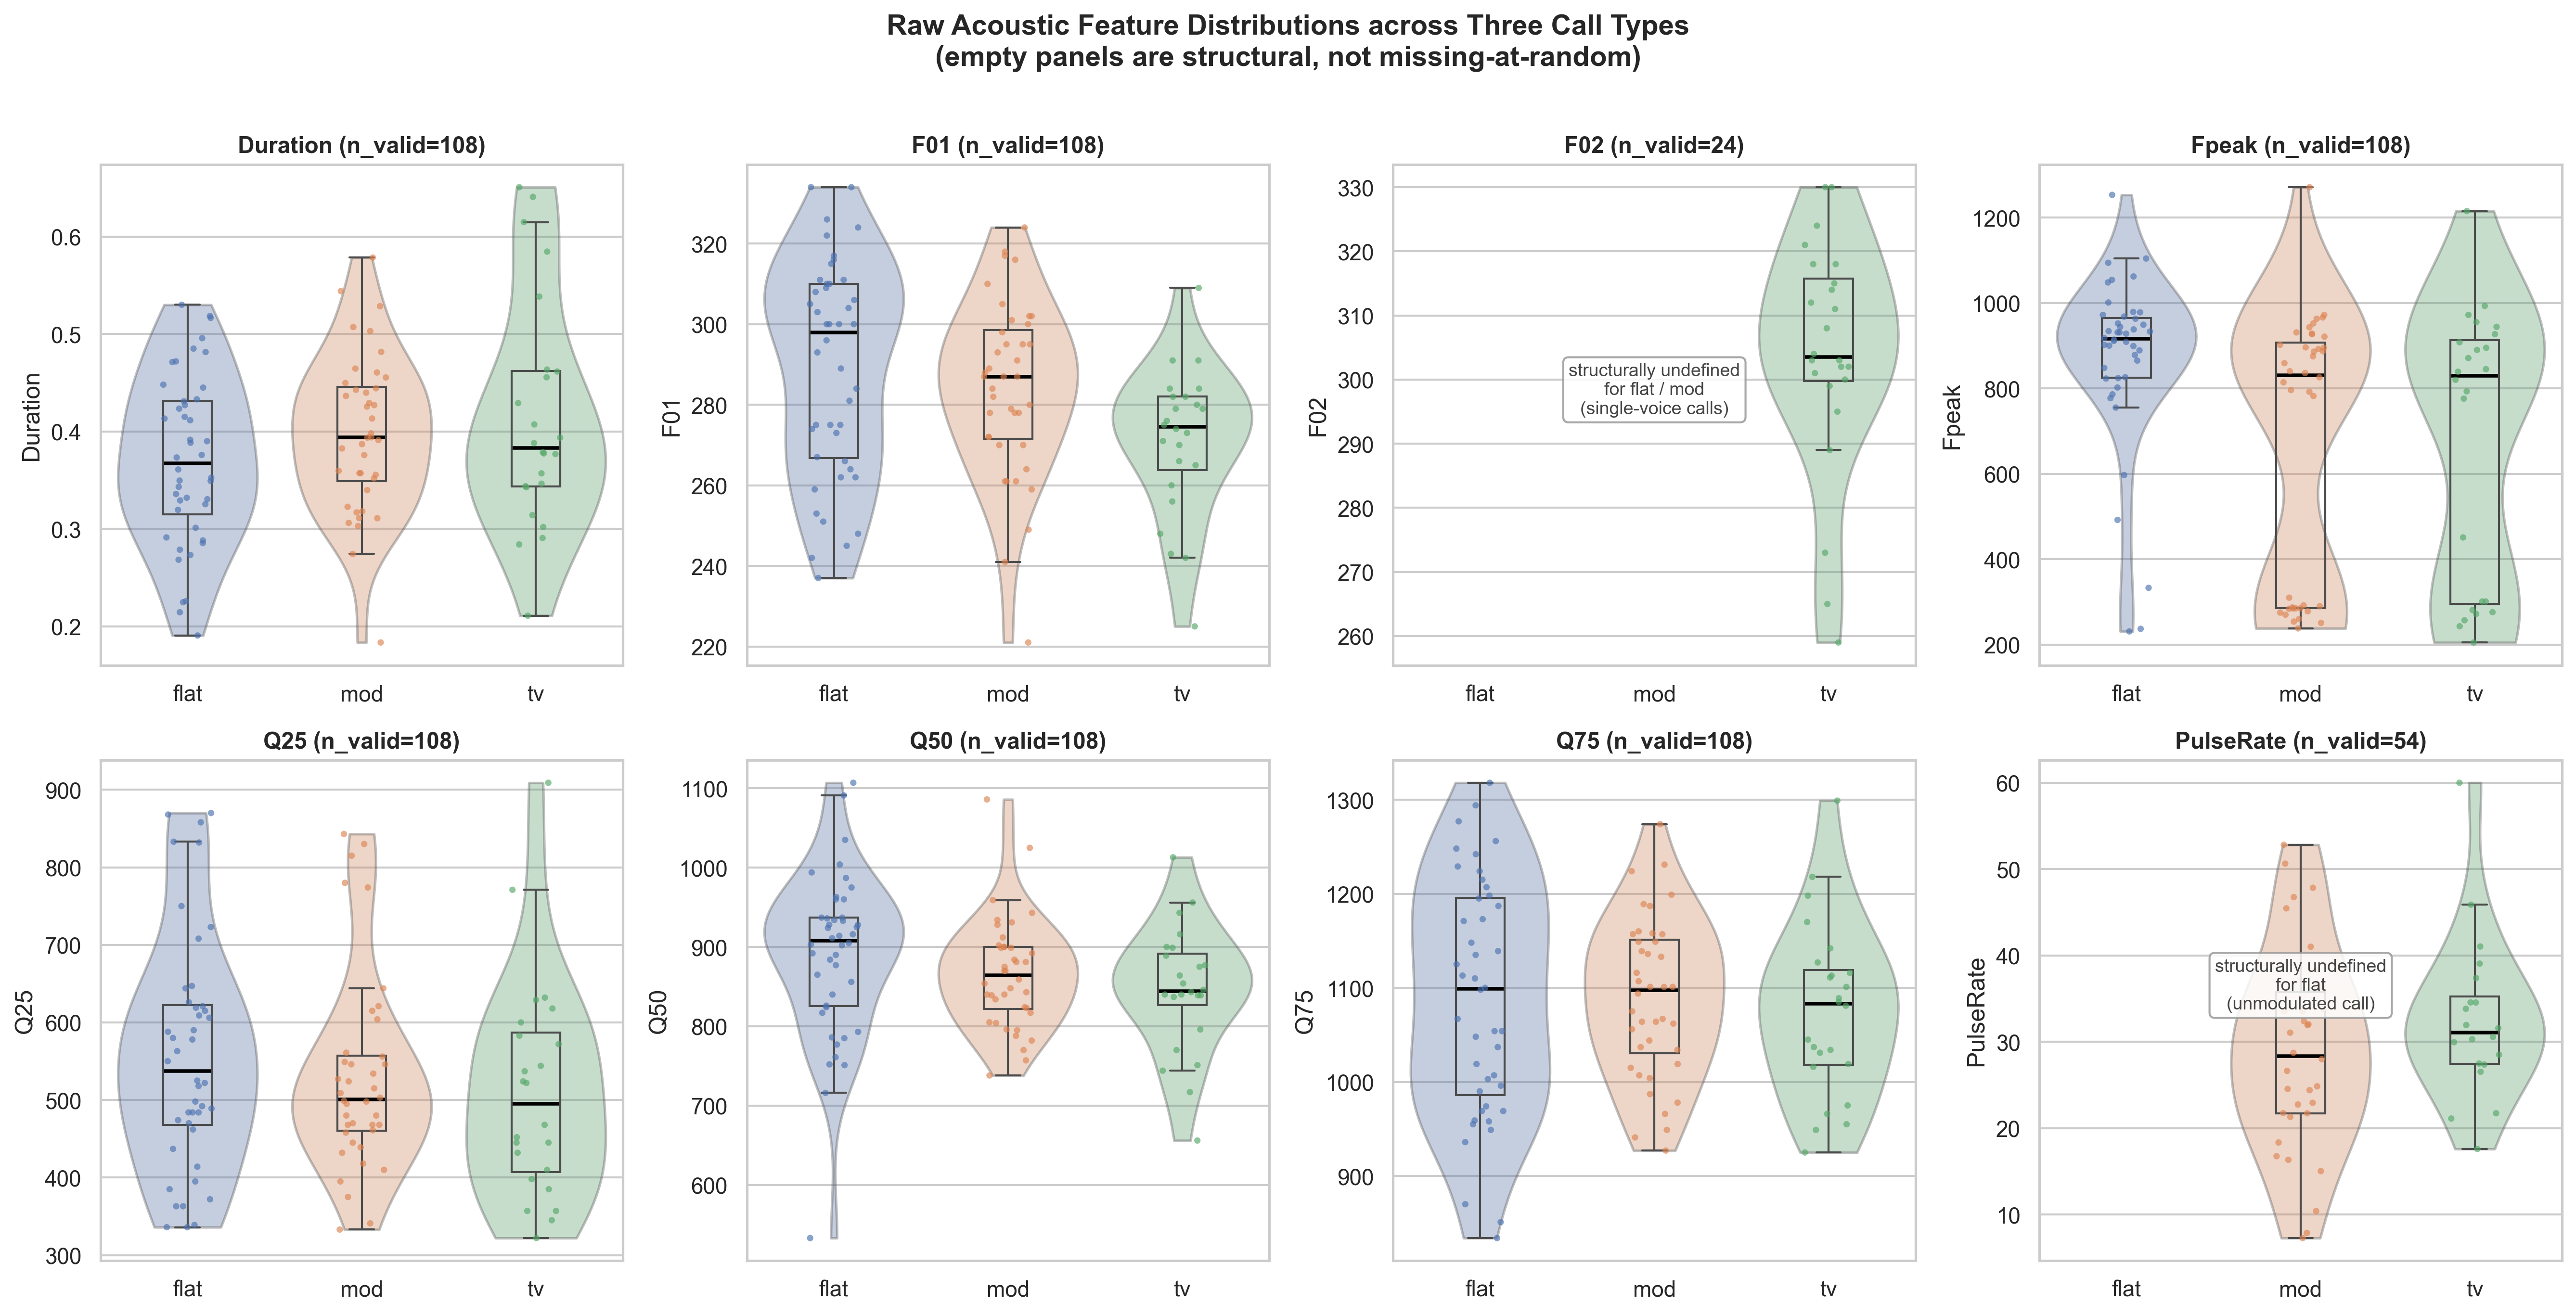
\includegraphics[width=0.86\textwidth]{../outputs_p1/P1_fig1_raw_distributions.png}
    \caption{三类海面叫声 $8$ 项原始声学特征分布（标注框为结构性未定义特征）}
    \label{fig:p1_raw}
\end{figure}


（1）\textbf{\texttt{Fpeak} 双峰混合}：由图~\ref{fig:p1_engineered}，\texttt{flat} 几乎全在三倍频达峰（\texttt{PeakAtFundamental} 仅 $0.068$），而 \texttt{mod}（$0.375$）与 \texttt{tv}（$0.333$）
约三分之一在基频达峰，能量主峰是“离散跳档”的违背正态分布假设，同时也会干扰分类器的特征归因导致；
\begin{figure}[htbp]
    \centering
    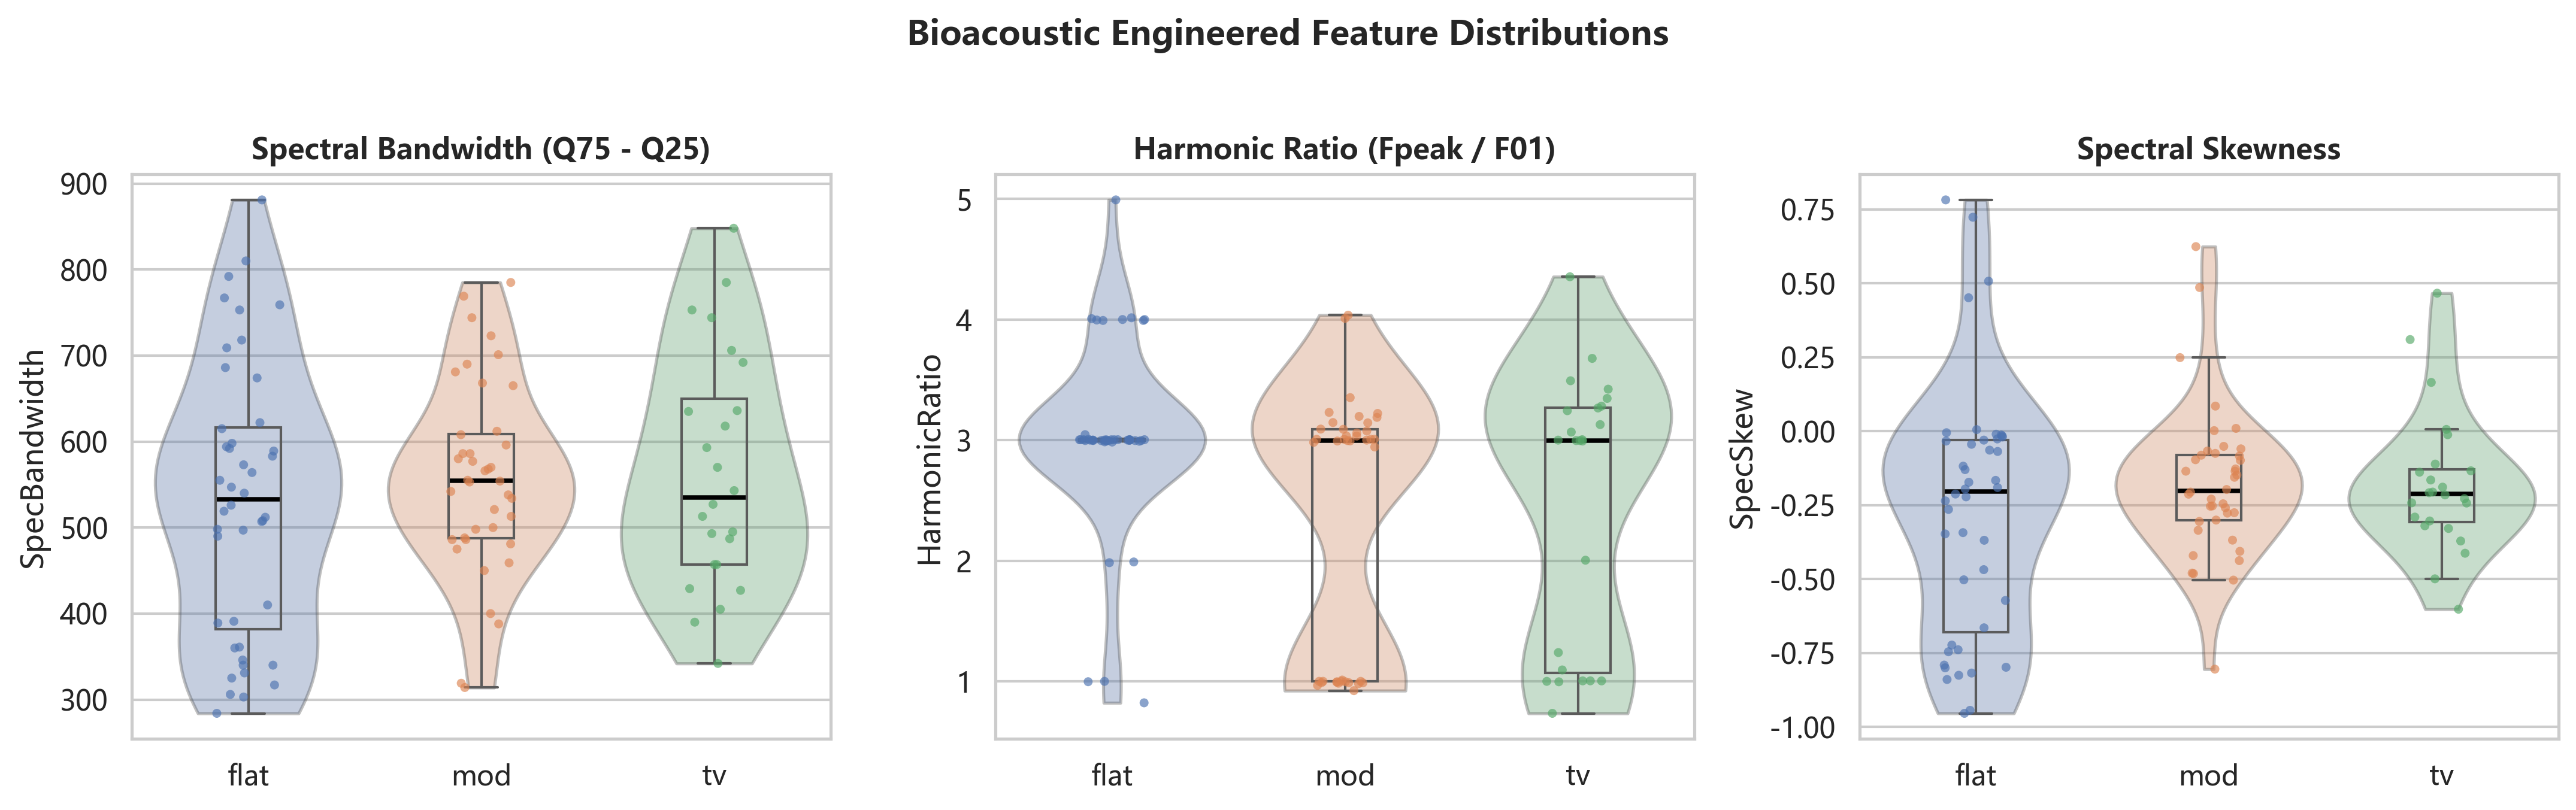
\includegraphics[width=.92\linewidth]{../outputs_p1/P1_fig2_engineered_distributions.png}
    \caption{衍生特征分布与 \texttt{Fpeak}/\texttt{F01} 双峰诊断}
    \label{fig:p1_engineered}
\end{figure}

（2）\textbf{高度共线性}：由图~\ref{fig:p1_collinearity}，按 $\text{VIF}_j = (1 - R_j^2)^{-1}$ 诊断 $10$ 维特征空间，
共有 $4$ 对强相关（$|\rho| \ge 0.7$）、$8$ 个特征 $\text{VIF} > 10$（\texttt{Q25}、\texttt{Q75}、\texttt{SpecBandwidth} 为 $\infty$，$\text{VIF}_{\text{Fpeak}} = 185.27$，
$\text{VIF}_{\text{HarmonicRatio}} = 156.10$），条件数达 $6.3 \times 10^{16}$，
因此多元检验应当回归非冗余 $6$ 维基础空间。


\begin{figure}[htbp]
    \centering
    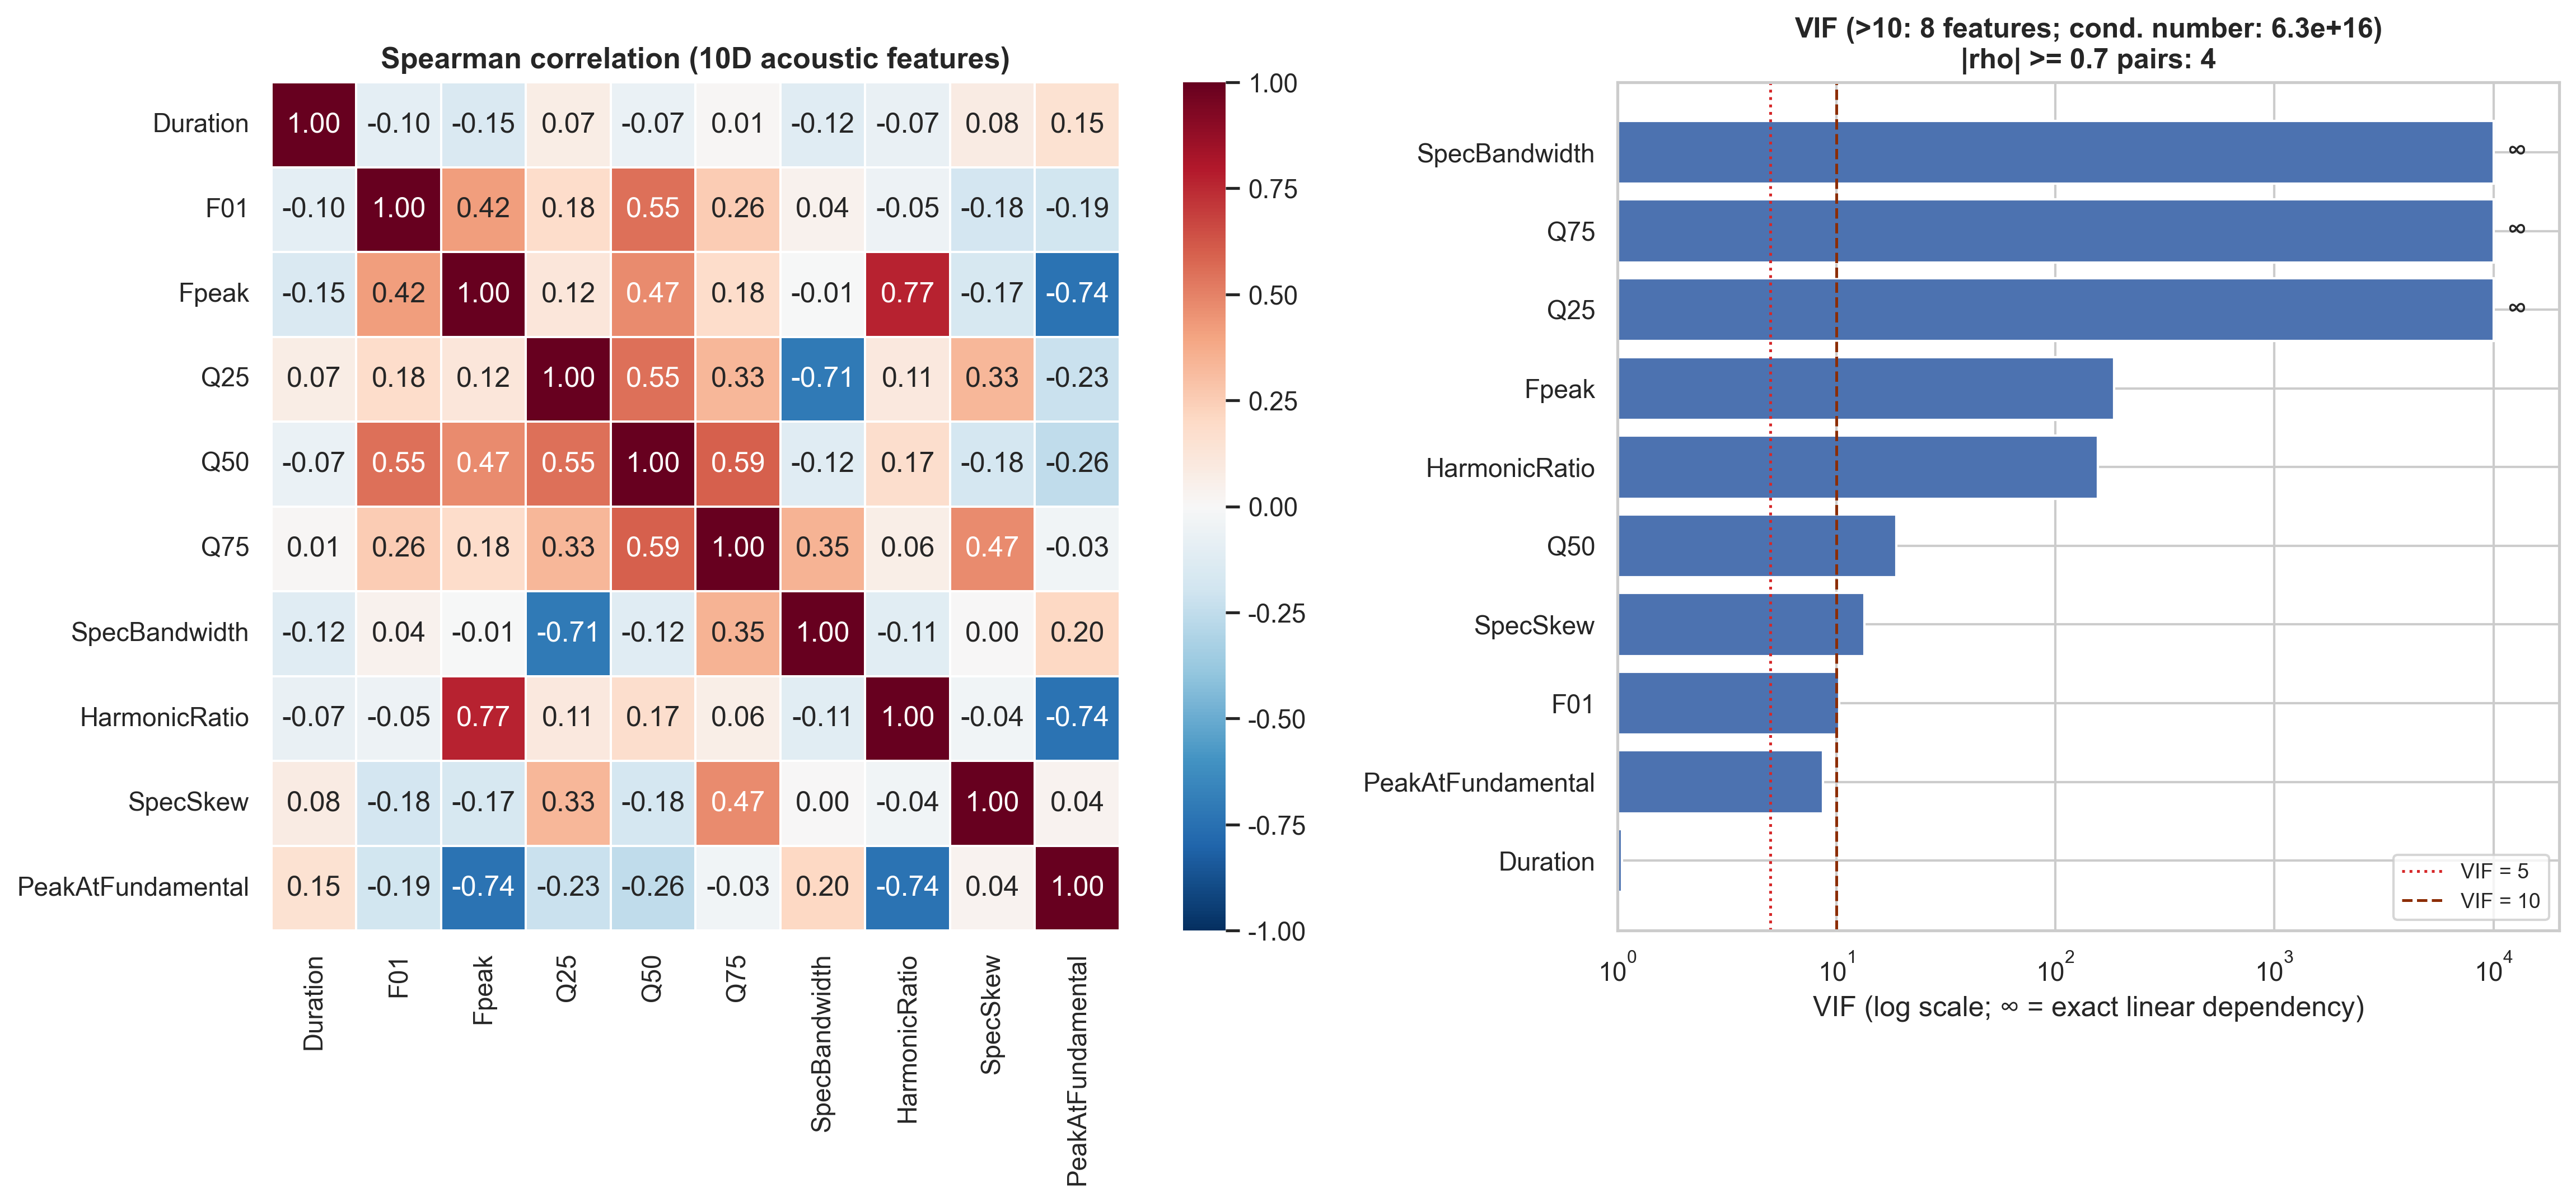
\includegraphics[width=\linewidth]{../outputs_p1/P1_fig3_spearman_heatmap.png}
    \caption{声学特征的 Spearman 相关热图与方差膨胀因子（VIF）诊断}
    \label{fig:p1_collinearity}
\end{figure}

\subsection{日期校正单变量非参数检验与 6D 多元空间检验}

鉴于特征非正态且 $108$ 条叫声采自 $16$ 个采样日期（存在批次伪重复），我们并行采用\textbf{单变量非参数检验（Kruskal--Wallis 与 Mann--Whitney $U$）}及\textbf{多变量置换多元方差分析（PERMANOVA 与 PERMDISP）}：

\subsubsection{Kruskal--Wallis 与日期中心化分层置换检验}

置换次数为 $N_{\text{perm}}=2999$。对 $9$ 项连续特征做全局 Holm 校正，计算效应量 $\varepsilon^2$，并以日期内中心化 $\tilde{x}_{id}$ 剥离日期效应；两两事后比较采用全局 $27$ 次 Holm 校正的 Mann--Whitney $U$ 检验及秩双列相关效应量 $r$（配合日期簇自助法 CI）：
\begin{equation}
    \varepsilon^2 = \max\!\left(0,\; \frac{H - k + 1}{n - k}\right), \qquad
    \tilde{x}_{id} = x_{id} - \bar{x}_d, \qquad
    r = \frac{2U}{n_1 n_2} - 1.
\end{equation}

结果显示，朴素检验仅 \texttt{Fpeak} 显著（$p_{\text{holm}} = 0.0194$，截断极端值后 $p_{\text{trimmed}} = 0.0002$），\texttt{F01} 不显著（$p_{\text{holm}} = 0.0827$）；
加入日期校正后，\textbf{\texttt{F01} 成为唯一跨日期稳健显著的特征}（$p_{\text{holm\_date}} = 0.0210$），
\texttt{Fpeak} 不再显著（$0.1520$）。
朴素仅 \texttt{Fpeak}（\texttt{flat} vs. \texttt{mod}，$p_{\text{holm}} = 0.0346, r = 0.4091$）显著；日期校正后仅 \texttt{F01}（\texttt{flat} vs. \texttt{tv}，$p_{\text{holm\_date}} = 0.0405, r = 0.3968$）显著（见图~\ref{fig:p1_test} 左）。\texttt{PulseRate} 在 \texttt{mod} 与 \texttt{tv} 间无显著差异（$p_{\text{holm\_date}} = 0.1337$）。

\subsubsection{非冗余 6D 空间的 PERMANOVA 与 PERMDISP 检验}

结合 PCA 双标图，基于标准化 6D 欧氏距离矩阵 $d_{ij}$ 检验质心分离与离散度齐性：
\begin{equation}
    \begin{aligned}
        SS_T &= \frac{1}{2n}\sum_{i,j} d_{ij}^2, \\
        SS_W &= \sum_{g=1}^{k}\frac{1}{2n_g}\sum_{i,j \in G_g} d_{ij}^2, \\
        \text{Pseudo-}F &= \frac{(SS_T - SS_W)/(k-1)}{SS_W/(n-k)}, \\
        R^2 &= 1 - \frac{SS_W}{SS_T}.
    \end{aligned}
\end{equation}
三类叫声整体质心显著分离（$\text{Pseudo-}F = 2.6884, R^2 = 0.0487, p = 0.0083$）且离散度齐性满足（$\text{PERMDISP } p = 0.8990$，见图~\ref{fig:p1_test} 右）；两两差异主要来自 \texttt{flat} vs. \texttt{tv}（$p_{\text{holm}} = 0.0080, R^2 = 0.0599$），\texttt{flat} vs. \texttt{mod} 处于临界值（$p_{\text{holm}} = 0.0500$），\texttt{mod} vs. \texttt{tv} 无显著差异（$0.2527$）。

\begin{figure}[htbp]
    \centering
    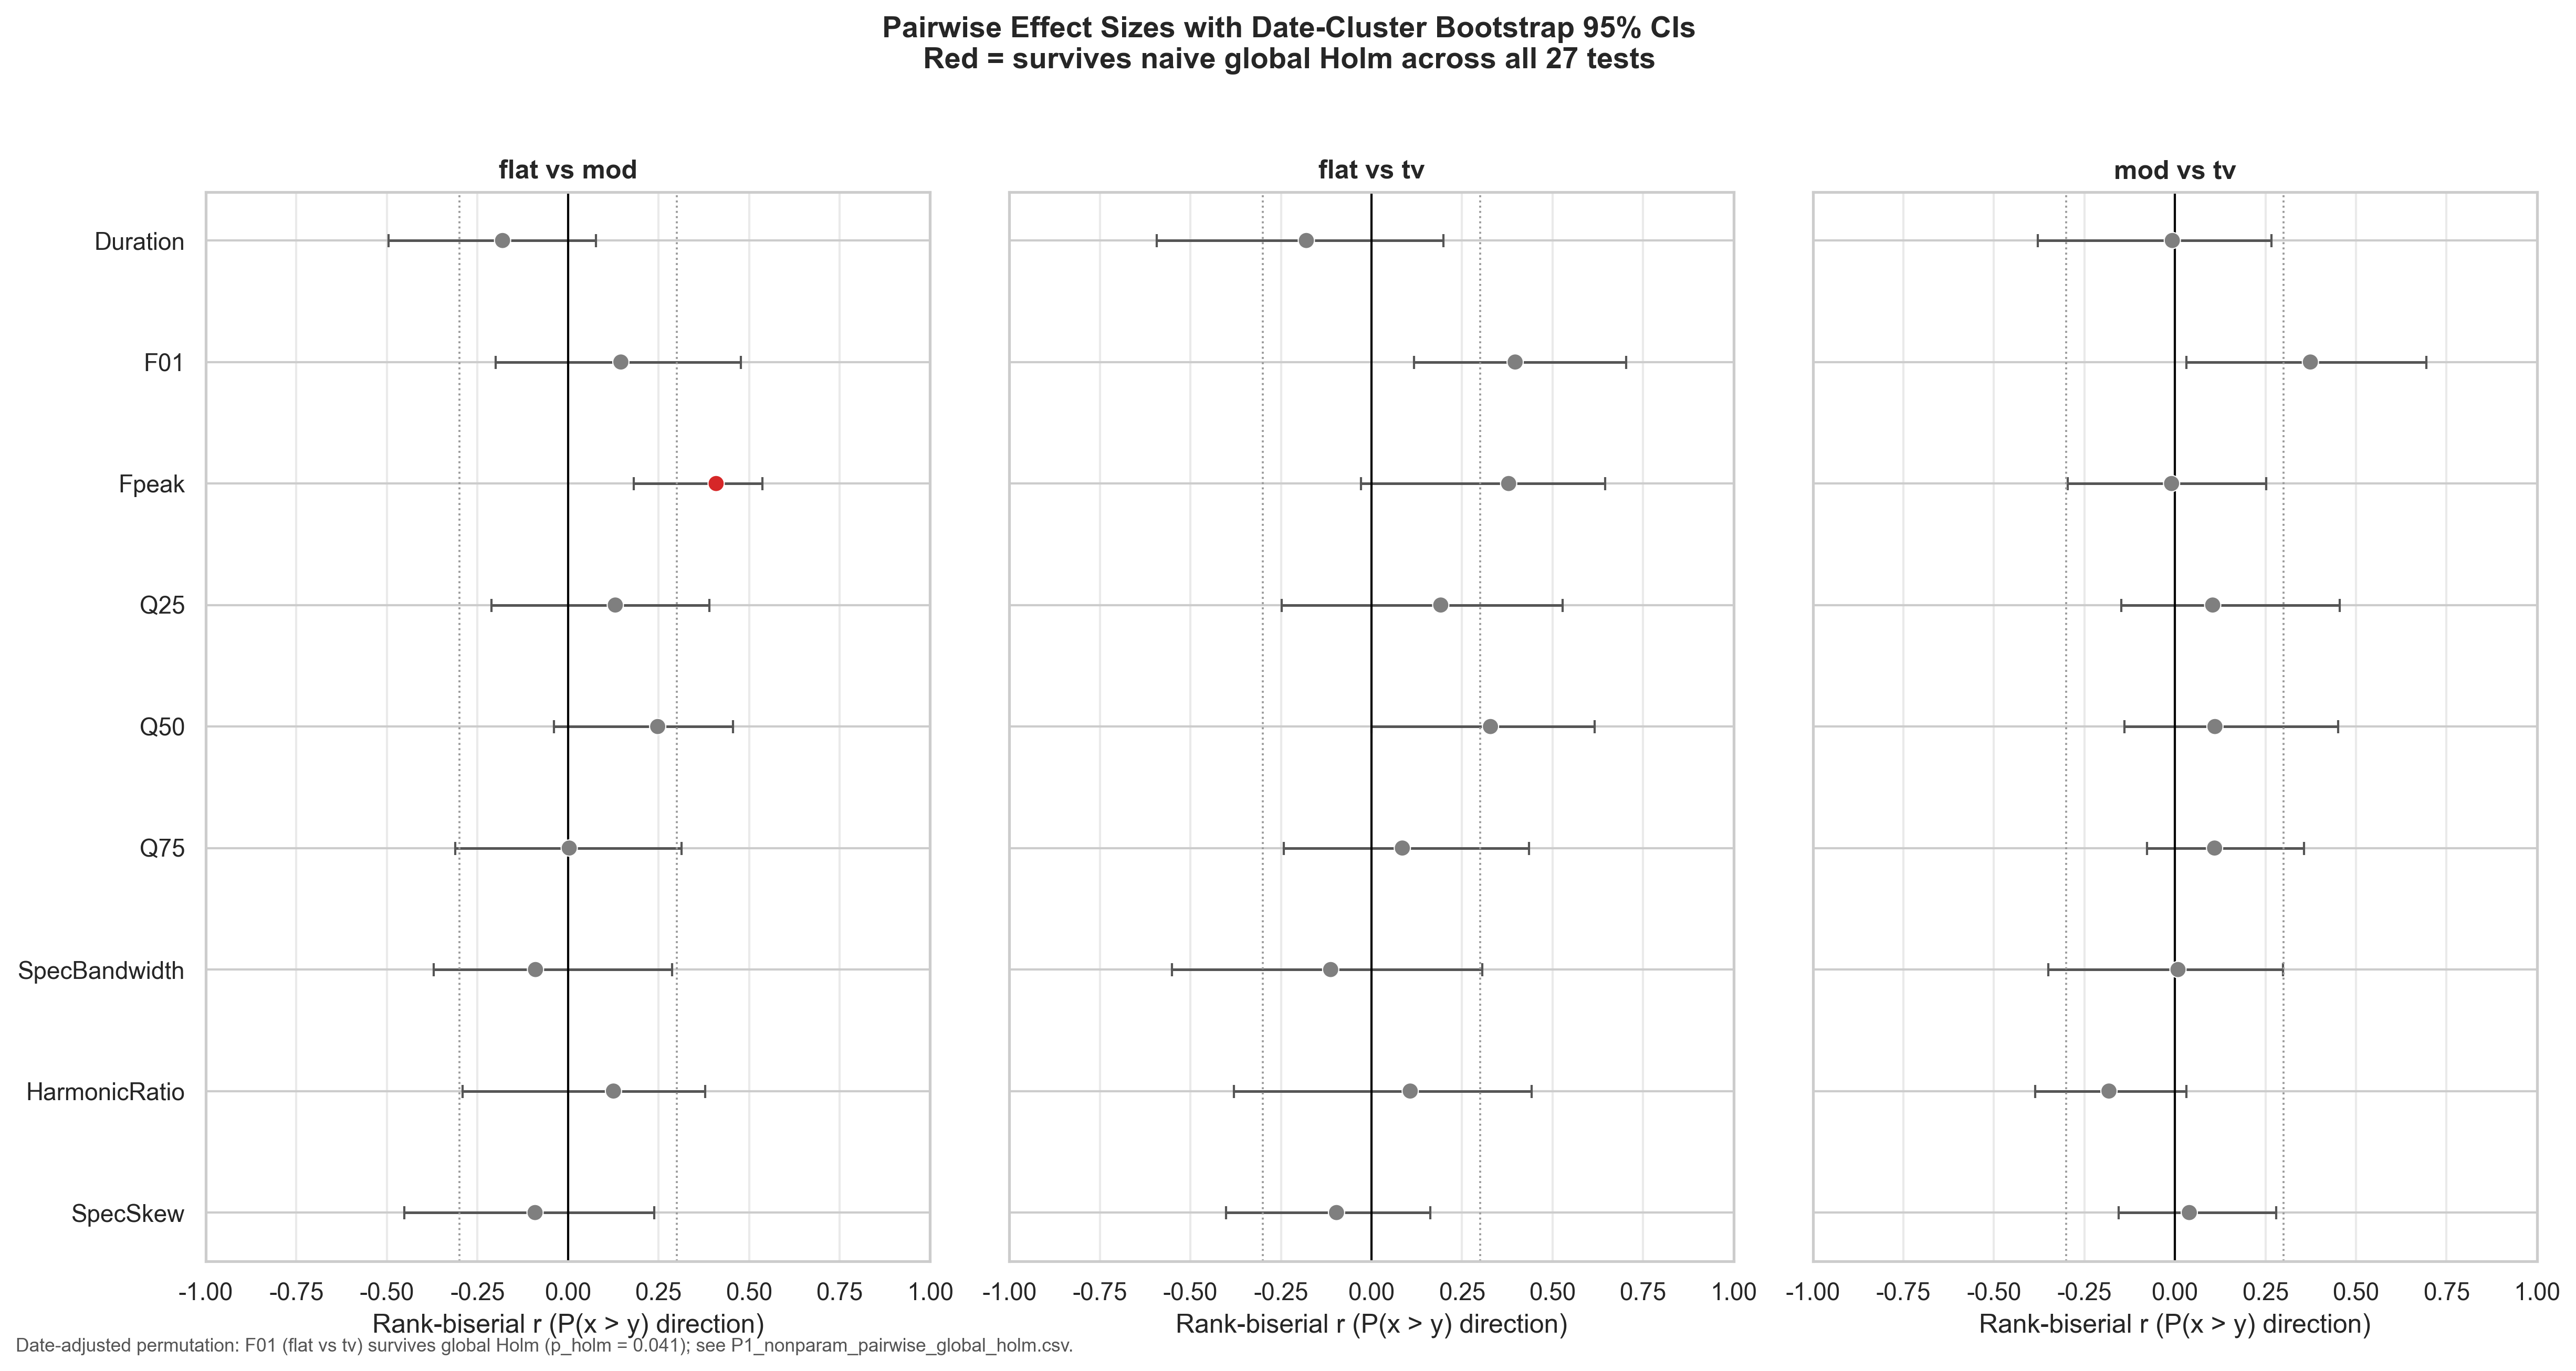
\includegraphics[height=.31\linewidth]{../outputs_p1/P1_fig12_effect_size_forest.png}\hfill
    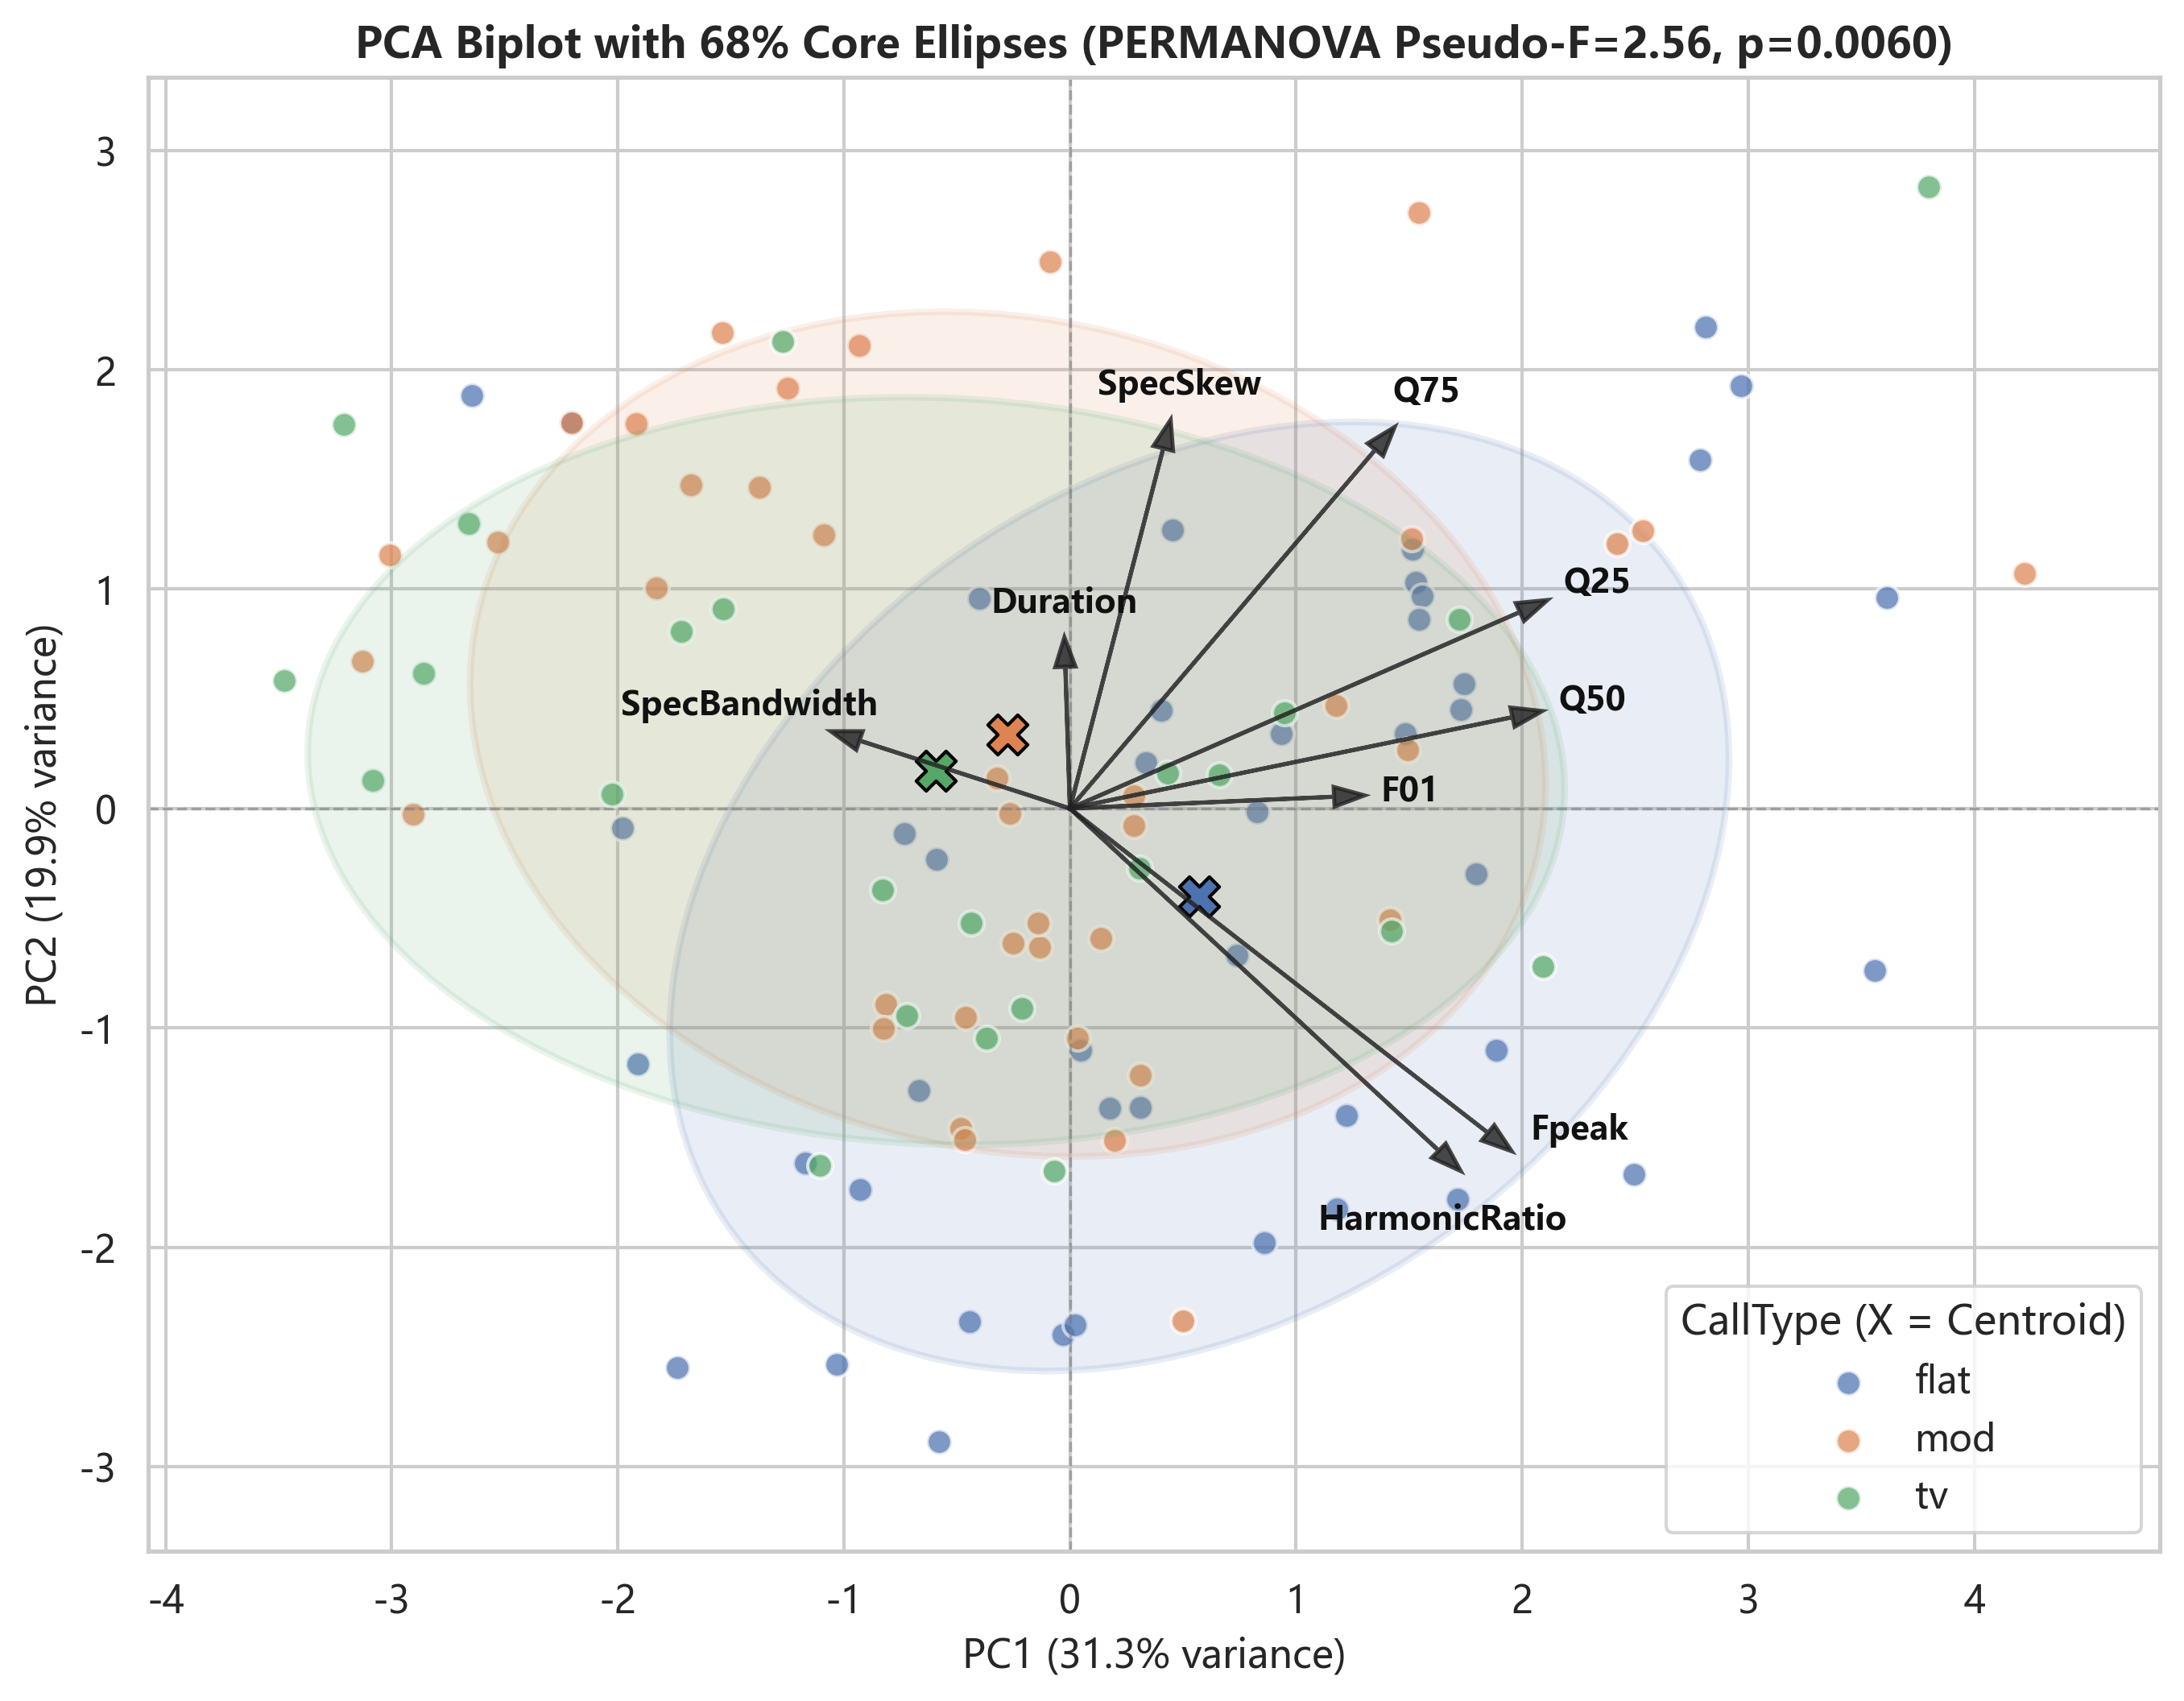
\includegraphics[height=.31\linewidth]{../outputs_p1/P1_fig4_PCA_PERMANOVA_biplot.png}
    \caption{两两 Mann--Whitney 效应量森林图（左）与 6D 非冗余空间 PCA--PERMANOVA 双标图（右）}
    \label{fig:p1_test}
\end{figure}

单变量与多变量非参数检验共同表明，
三类叫声在连续声学特征上存在统计显著但幅度有限的差异。
剔除采样日期伪重复后，\texttt{F01} 是唯一跨日期稳健显著的单变量差异（主要表现为 \texttt{flat} 高于 \texttt{tv}），
而 \texttt{Fpeak} 的表面显著性受采样日期驱动；
在非冗余 $6$ 维空间中，三类质心整体显著分离（$p = 0.0083$），
但解释方差仅 $4.87\%$（\texttt{mod} 与 \texttt{tv} 无显著分离），
因此我们认为仅依赖连续声学汇总特征难以实现高精度三分类，还需通过后续防泄露消融实验与分层分类加以验证。

\subsection{基于消融验证、两阶段分层分类器的分类建模}

\subsubsection{五组特征消融实验与目标泄露剥离}

为验证阶段二关于``纯连续特征难以实现高精度三分类''的预判，并量化结构性缺失引入的目标泄露，我们在 $10$ 维纯声学特征与 $2$ 维定义标志上构造了五组递进特征空间：
\begin{equation}
    \begin{gathered}
        \mathcal{X}_1 = \{\text{6D 基础特征}\},\qquad
        \mathcal{X}_2 = \mathcal{X}_1 \cup \{\text{SpecBandwidth, HarmonicRatio, SpecSkew}\}, \\
        \mathcal{X}_3 = \mathcal{X}_2 \cup \{\text{PeakAtFundamental}\},\qquad
        \mathcal{X}_{\text{def}} = \{\text{F02\_present, PulseRate\_present}\},\qquad
        \mathcal{X}_4 = \mathcal{X}_3 \cup \mathcal{X}_{\text{def}}.
    \end{gathered}
\end{equation}
在五组特征空间上，分别训练\textbf{LASSO 惩罚多项逻辑回归（LASSO-Logit）}与\textbf{平衡随机森林（Balanced Random Forest）}，采用 $10 \times 5$ 重复分层交叉验证（$J=50$ 折，多数类基线 $0.407$，分层随机基线 $0.353$）及按采样日期分组的 \texttt{StratifiedGroupKFold} 进行评估，并以多分类 Brier 分数与 Nadeau--Bengio 校正重采样 $t$ 检验度量校准度与模型差异：
\begin{equation}
    \text{Brier} = \frac{1}{n}\sum_{i=1}^{n}\sum_{c=1}^{3}\bigl(\hat{p}_{ic} - y_{ic}\bigr)^2, \qquad
    t_{\text{corr}} = \frac{\bar{\Delta}}{\sqrt{\left(\frac{1}{J} + \frac{n_{\text{test}}}{n_{\text{train}}}\right) s_\Delta^2}},
\end{equation}
其中 $\hat{p}_{ic}$ 为样本 $i$ 预测属第 $c$ 类的概率，$y_{ic} \in \{0,1\}$ 为真实类别指示位，$\bar{\Delta}$ 与 $s_\Delta^2$ 为两模型在 $J$ 折上的准确率差值均值与方差。

消融结果显示：仅使用 $\mathcal{X}_{\text{def}}$（2D 定义标志）即可达到 $0.945$ 的准确率（$\mathcal{X}_4$ 加入全部声学特征后为 $0.931$--$0.945$），直接证明约 $94\%$ 的高准确率源于类别定义的同义反复（目标泄露），而非声学特征可分性。剥离泄露标志后，纯声学 10D 模型（$\mathcal{X}_3$）中随机森林的 $10 \times 5$ CV 准确率仅为 $0.538\,[0.509, 0.566]$（Macro-F1 $= 0.484$，OvR AUC $= 0.737$，Brier $= 0.548$），LASSO-Logit 为 $0.470$（Brier $= 0.636$）；在按采样日期分组的 \texttt{StratifiedGroupKFold} 下，随机森林准确率进一步降至 $0.432$（LASSO 为 $0.512 \pm 0.256$），证实仅凭现有连续汇总特征无法直接实现高精度三分类。

\subsubsection{两阶段分层分类器的构建与求解}

鉴于 \texttt{F02} 物理定义了对双声叫声 \texttt{tv} 的识别，为在杜绝目标泄露的前提下构建实用分类器，我们将``物理定义判别''与``纯声学机器学习''解耦，设计两阶段分层分类框架：
\begin{itemize}
    \item \textbf{第一层（Stage 1：显式物理定义规则）}：直接依据第二基频是否存在分离双声叫声 \texttt{tv}，即 $\hat{y}_1(\mathbf{x}) = \texttt{tv} \iff \text{F02\_present} = 1$（覆盖全部 $24$ 条 \texttt{tv} 样本，准确率为 $1.000$，显式声明为物理定义规则而非学习模型）。
    \item \textbf{第二层（Stage 2：单声道纯声学二分类）}：对剩余单声道样本集合 $\mathcal{S}_2 = \{i : \text{F02\_present}_i = 0\}$（\texttt{flat} $44$ 条 vs. \texttt{mod} $40$ 条，多数类基线 $0.524$），在 $10$ 维无泄露声学特征 $\mathbf{x}_{10\text{D}}$ 上对比 $L_1$ 正则化逻辑回归（LASSO-Logit）与 $B=300$ 棵决策树软投票的平衡随机森林：
    \begin{equation}
        \min_{\mathbf{w},\,b} -\sum_{i \in \mathcal{S}_2}\Bigl[z_i \ln \hat{p}_i + (1 - z_i)\ln(1 - \hat{p}_i)\Bigr] + \frac{1}{C}\|\mathbf{w}\|_1, \qquad
        \hat{P}_{\text{RF}}\bigl(c \mid \mathbf{x}_{10\text{D}}\bigr) = \frac{1}{B}\sum_{b=1}^{B} \hat{p}_b\bigl(c \mid \mathbf{x}_{10\text{D}}\bigr),
    \end{equation}
    其中 $z_i = \mathbb{I}(y_i = \texttt{mod})$，$\hat{p}_i = \operatorname{expit}(\mathbf{x}_{i,10\text{D}}^\top \mathbf{w} + b)$，$\hat{p}_b$ 为第 $b$ 棵类别平衡决策树的后验概率预测。
\end{itemize}
联立两层可得最终分层决策函数：
\begin{equation}
    \hat{y}(\mathbf{x}) =
    \begin{cases}
        \texttt{tv}, & \text{F02\_present} = 1\;\text{（Stage 1：定义规则）}, \\[4pt]
        \arg\max\limits_{c \in \{\texttt{flat},\,\texttt{mod}\}} \hat{P}_{\text{Stage2}}\bigl(c \mid \mathbf{x}_{10\text{D}}\bigr), & \text{F02\_present} = 0\;\text{（Stage 2：纯声学分类）}.
    \end{cases}
\end{equation}
实测结果表明，在真正具有声学难度的 Stage 2（\texttt{flat} vs. \texttt{mod}）上，平衡随机森林的 $10 \times 5$ CV 准确率提升至 $0.749$（Balanced Accuracy $= 0.748$，AUC $= 0.830$），显著优于 LASSO-Logit（$0.596$，AUC $= 0.590$）；两阶段组合后的整体分类准确率达到 $0.815$（Balanced Accuracy $= 0.840$，见图~\ref{fig:p1_cls} 左）。

\begin{figure}[!ht]
    \centering
    \begin{minipage}[b]{0.54\textwidth}
        \centering
        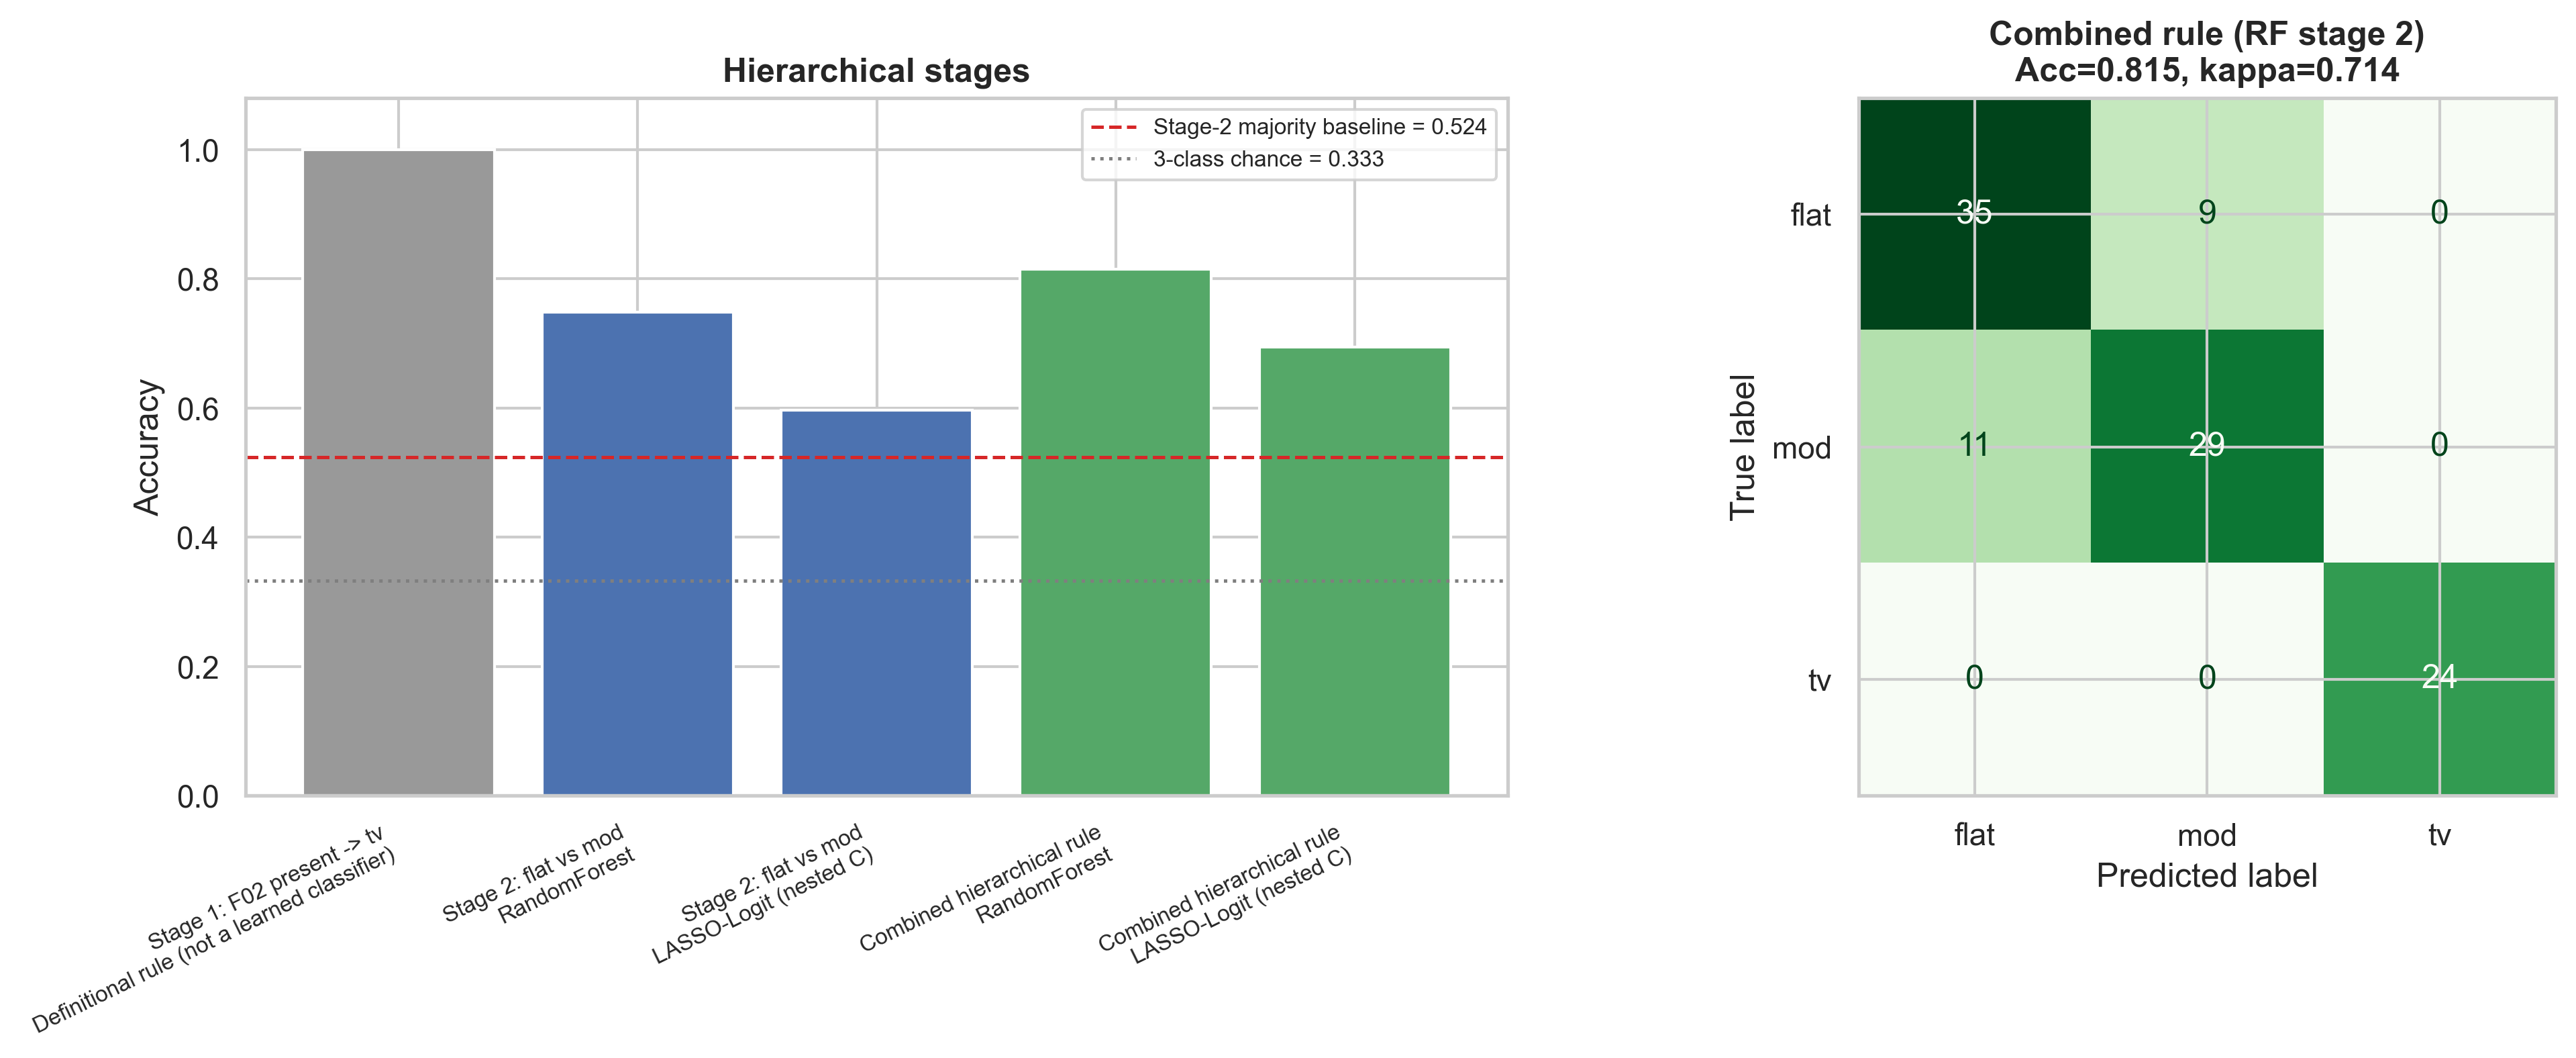
\includegraphics[width=\textwidth]{../outputs_p1/P1_fig11_hierarchical_classifier.png}
    \end{minipage}\hfill
    \begin{minipage}[b]{0.46\textwidth}
        \centering
        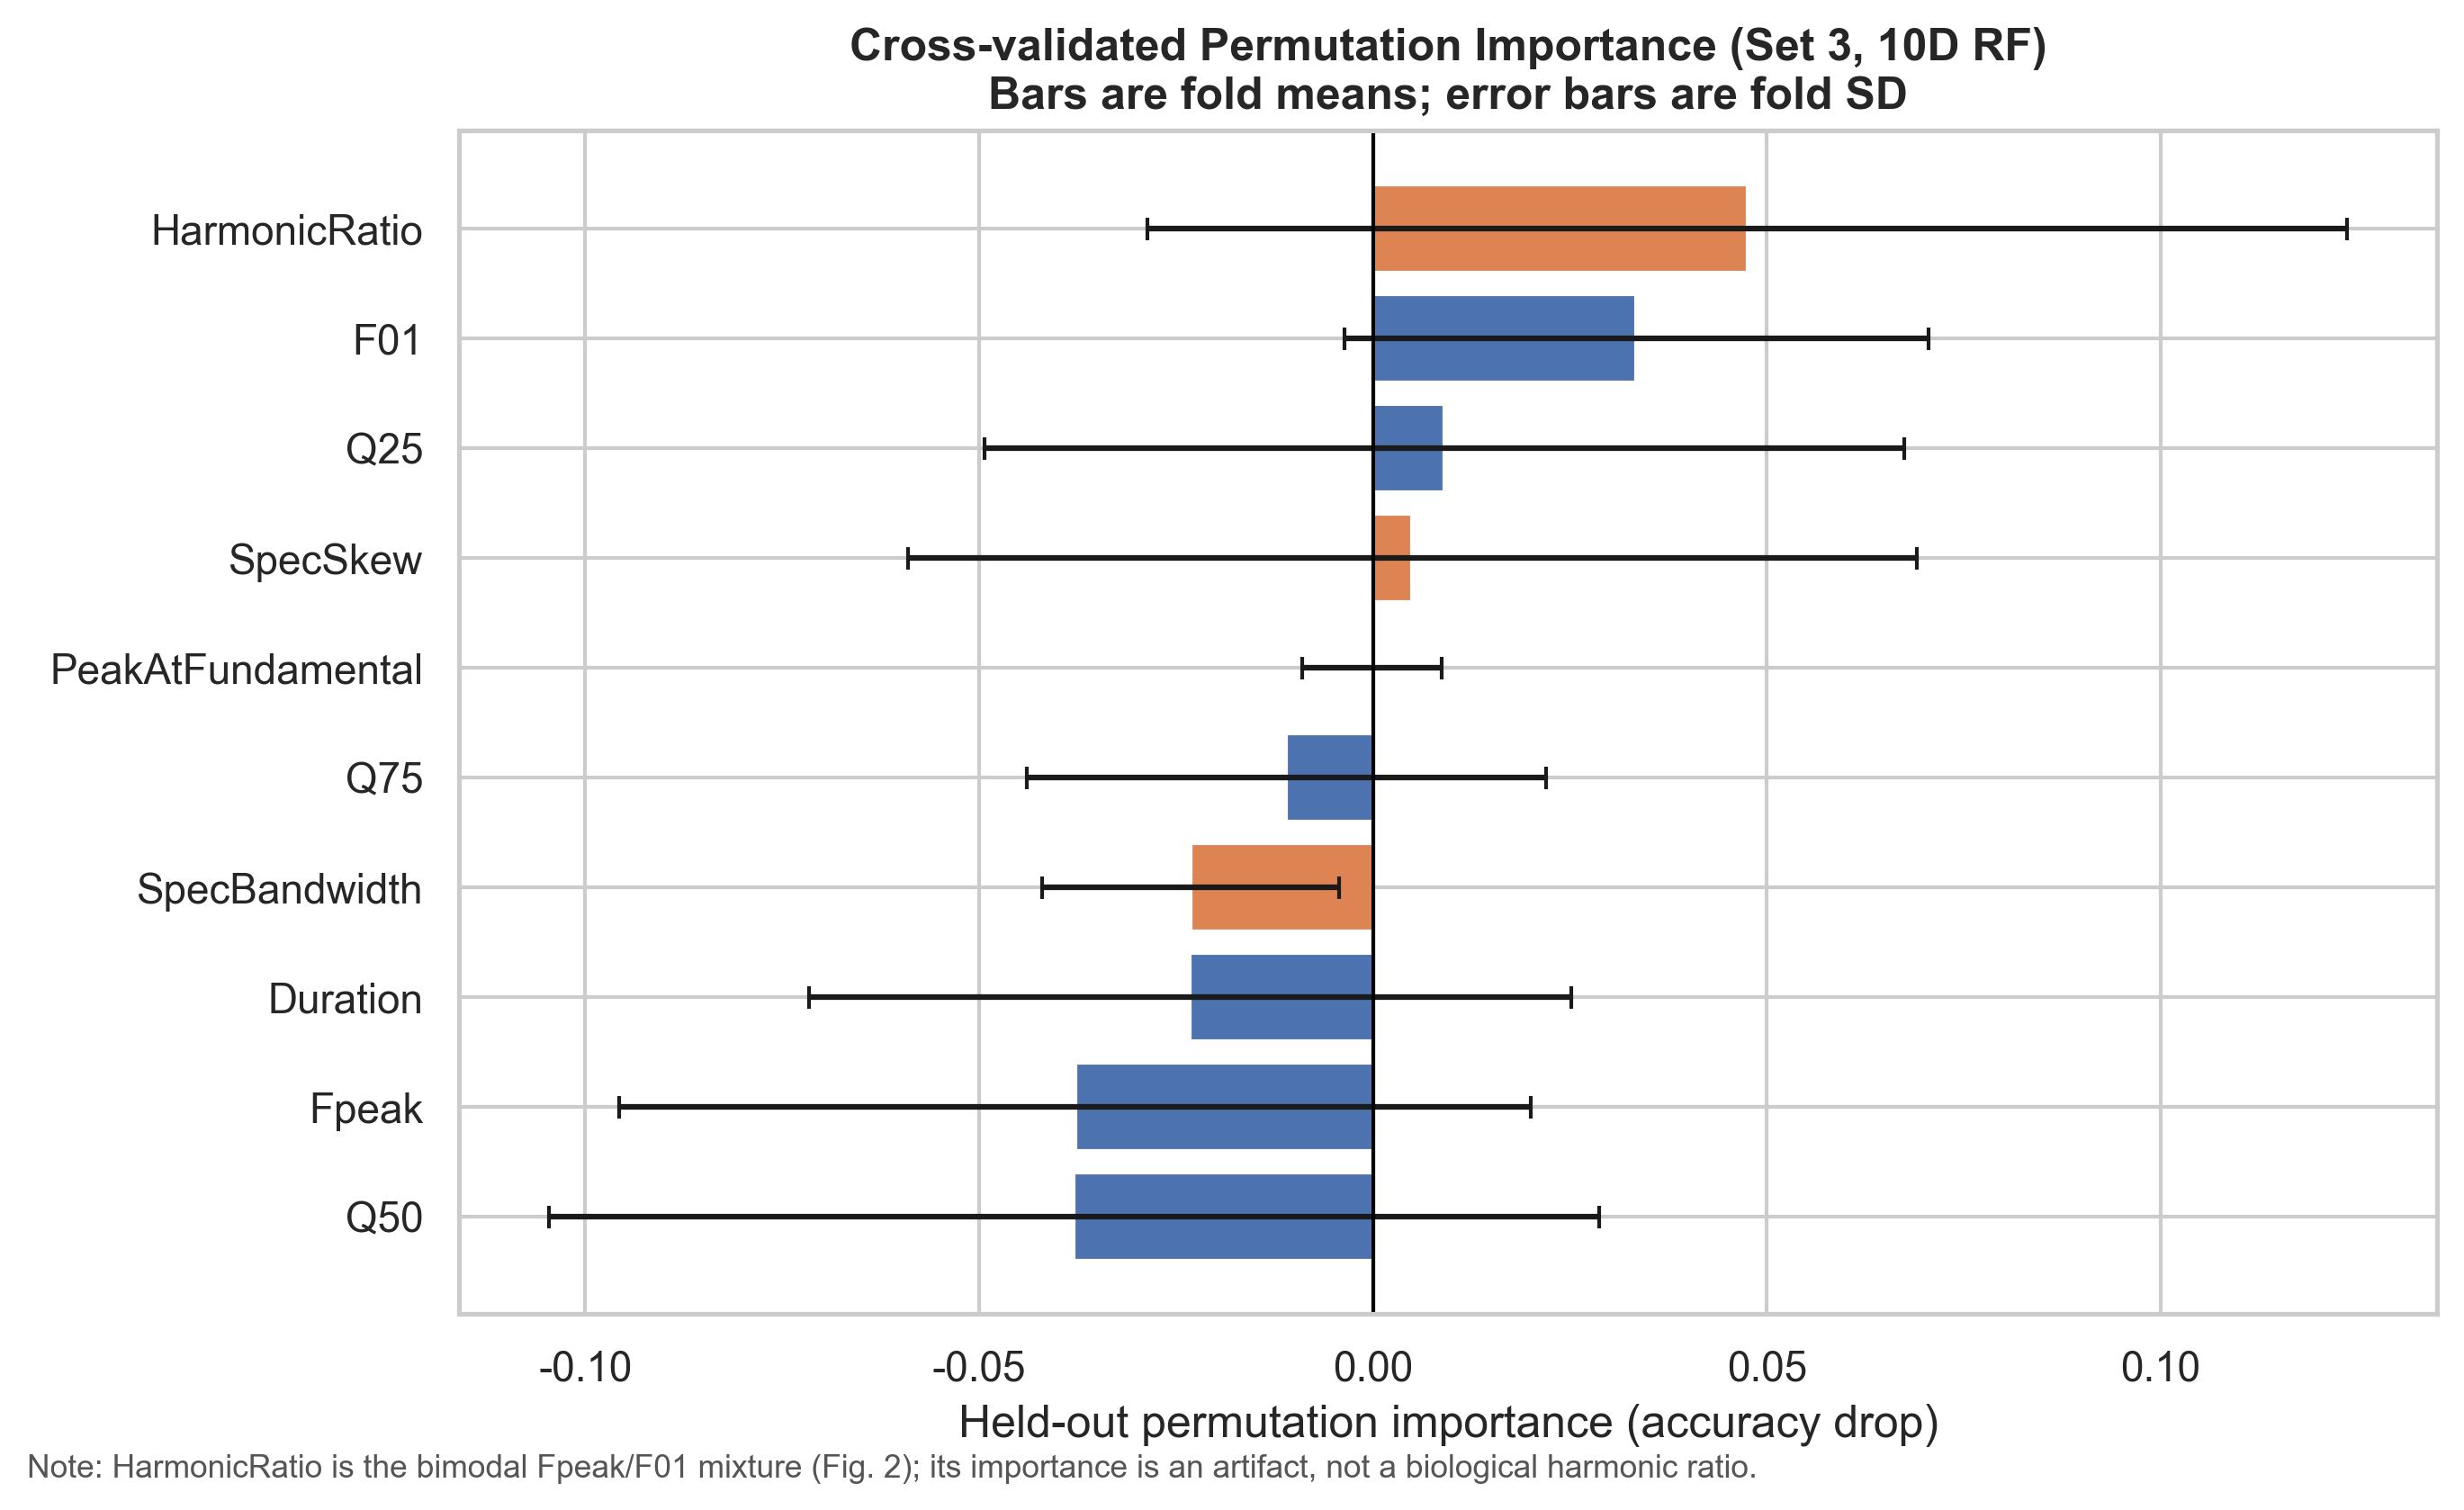
\includegraphics[width=\textwidth]{../outputs_p1/P1_fig13_permutation_importance.png}
    \end{minipage}
    \caption{两阶段分层分类器与组合混淆矩阵（左）及 Set 3 随机森林置换特征重要性（右）}
    \label{fig:p1_cls}
\end{figure}
\FloatBarrier

\subsubsection{主影响因子归因与特征排序}

为客观识别驱动叫声分类的主要声学影响因素，我们在 $\mathcal{X}_3$（10D 纯声学空间）上联合计算\textbf{交叉验证测试集置换重要性（CV Permutation Importance）}、\textbf{互信息（Mutual Information）}与\textbf{LASSO 自助法特征选择频率}：
\begin{equation}
    \text{PI}_j = \frac{1}{K}\sum_{k=1}^{K}\left(\text{Acc}_k - \frac{1}{M}\sum_{m=1}^{M}\text{Acc}_{k,\,\pi_j^{(m)}}\right), \qquad
    I(X_j; Y) = \sum_{y}\int p(x_j, y)\ln\frac{p(x_j, y)}{p(x_j)p(y)}\,\mathrm{d}x_j,
\end{equation}
其中 $\text{Acc}_k$ 为第 $k$ 折验证集原始准确率，$\text{Acc}_{k,\,\pi_j^{(m)}}$ 为将该折中第 $j$ 个特征随机置换第 $m$ 次后的准确率。综合三项指标排序（见图~\ref{fig:p1_cls} 右）：\texttt{HarmonicRatio} 虽在置换重要性（$0.048$）与互信息（$0.332$）中排首位，但由阶段一已证其为 \texttt{Fpeak}/\texttt{F01} 双峰混合测量伪影，不作生物学归因；剔除该伪影后，真实声学影响因子的排序依次为：\textbf{第一，\texttt{F01}}（置换重要性 $0.033$，互信息 $0.139$，LASSO 选择频率 $0.775$，且为唯一通过日期校正检验的稳健特征）；\textbf{第二，\texttt{PeakAtFundamental}}（LASSO 选择频率 $0.665$，直接刻画基频与三倍频的能量峰值模态切换）；其余特征（如 \texttt{Q25}、\texttt{SpecSkew}、\texttt{Duration}、\texttt{Q50}、\texttt{Q75}）的测试集置换重要性接近零或为负，边际贡献微弱。



至此，我们通过将 \texttt{tv} 的物理定义判别与 \texttt{flat} vs. \texttt{mod} 纯声学二分类（随机森林 $0.749$，AUC $= 0.830$）解耦，
两阶段分层分类器在避免目标泄露的前提下实现了 $0.815$ 的综合准确率；多方法归因进一步确立了 \texttt{F01} 与 \texttt{PeakAtFundamental} 的主导地位。

\subsection{信息功能、传播稳健性评估与关键指标筛选}

本阶段通过\textbf{混杂校正多变量 Logistic 回归}（按 \texttt{expID} 簇自助法估计 CI）及\textbf{对数插值交叉距离与信息保留度指数}，定量联动回放（\texttt{Data 02}）与传播数据（\texttt{Data 03}--\texttt{Data 11}）：
\begin{equation}
    \operatorname{logit}\,P(\text{Response}=1) = \beta_0 + \beta_1\,\text{CallType} + \beta_2\,\text{Context} + \beta_3\,\text{Distance} + \beta_4\,\text{Npenguins},
\end{equation}
\begin{equation}
    d_{50} = 2^{\,\log_2 d_i + \frac{0.5 - \bar{F}_i}{\bar{F}_{i+1} - \bar{F}_i}(\log_2 d_{i+1} - \log_2 d_i)}, \qquad
    \text{InfoRetention}_c(d) = \text{AUC}_{\text{OvR},\,c} \times \bar{F}_c(d).
\end{equation}

控制协变量后，三类自然叫声相对对照组（原始响应率 $0.129$）的校正优势比分别为：
\texttt{flat} $\text{OR} = 13.04\,[6.81, 36.21]$、\texttt{mod} $15.24\,[7.17, 50.44]$、\texttt{tv} $19.87\,[9.74, 67.45]$，表明自然叫声均能显著诱发响应，但三类间置信区间重叠。
传播复合保真度的 $50\%$ 交叉距离依次为 \texttt{flat} $= 84.7\text{ m}$、\texttt{mod} $= 144.6\text{ m}$、\texttt{tv} $= 169.7\text{ m}$；
结合纯声学 $\text{AUC}_{\text{OvR}}$（$0.819 / 0.724 / 0.683$）与 $128\text{ m}$ 保真度（$0.359 / 0.553 / 0.654$），
信息保留度排序为 \textbf{\texttt{tv}（$0.447$）$>$ \texttt{mod}（$0.400$）$>$ \texttt{flat}（$0.294$）}。综合上述实证证据，表~\ref{tab:p1_contract} 
给出了传递至后续问题的关键声学指标筛选方案。

\begin{table}[htbp]
\centering
\caption{第一问关键声学指标筛选结果及后续建模与解释用途}
\label{tab:p1_contract}
\footnotesize
\renewcommand{\arraystretch}{1.18}
\setlength{\tabcolsep}{3pt}
\begin{tabularx}{\linewidth}{@{}>{\raggedright\arraybackslash}p{.15\linewidth}>{\raggedright\arraybackslash}p{.18\linewidth}>{\raggedright\arraybackslash}p{.26\linewidth}>{\raggedright\arraybackslash}X@{}}
\toprule
\textbf{筛选层级} & \textbf{声学指标} & \textbf{第一问实证依据} & \textbf{后续问题用途（P2 / P3 / P4）} \\
\midrule
\multirow{4}{*}{核心入选} & \texttt{CallType} & 分层分类输出（总准确率 $0.815$） & P2 分组衰减建模、P3 行为响应与潜伏期核心输入 \\
 & \texttt{F01} & 日期校正后唯一稳健显著 ($p_{\text{holm}}=0.0210$) & P2 载波衰减与声吸收物理解释；P4 声源级分析 \\
 & \texttt{F02} & \texttt{tv} 定义特征 ($F_{02}/F_{01}\approx 1.11$，拍频 $\sim 30\text{ Hz}$) & P2 双声抗衰减机理；P4 远距离联络特征 \\
 & \texttt{PeakAt\allowbreak{}Fundamental} & 有效分离基频与三倍频达峰模态 & P2 频谱能量分布与低频抗衰减解释 \\
\midrule
\multirow{3}{*}{辅助参考} & \texttt{Fpeak} & 朴素显著 ($0.0194$)，日期校正不显著 ($0.1520$) & P2 语谱图与振幅谱相关性辅助解释 \\
 & \texttt{Q25} / \texttt{Q50} / \texttt{Q75} & 单变量不显著或受日期驱动 ($\text{VIF}>18$) & P2 频谱包络展宽与保真度背景描述 \\
 & \texttt{Duration} / \texttt{PulseRate} & 组间无显著差异（\texttt{flat} 无脉冲） & P2 包络衰减；P3 暴露窗口与潜伏期参考 \\
\midrule
明确剔除 & \texttt{HarmonicRatio} & 双峰混合测量伪影 ($\text{VIF}=156.1$) & \textbf{剔除}，不作为连续生物学谐波比解释 \\
\bottomrule
\end{tabularx}
\end{table}
\clearpage


\section{问题二：声信号传播衰减建模与有效通信距离评估}

针对海面声信号随距离衰减的量化与有效通信半径估计问题，本节按``保真度融合与前置诊断、多模型衰减拟合与优选、分级阈值与双视角测距、多维敏感性与稳健性评判''四个阶段依次展开建模。

\subsection{多指标融合与前置诊断}

本阶段采用\textbf{主成分分析（PCA）加权融合模型}构建复合声学保真度指数 $F(d)$，并引入\textbf{等权平均}、\textbf{熵权法}
与\textbf{加权几何平均}作为对照。
基于 \texttt{Data 03}--\texttt{Data 11}（每类叫声 $300$ 条试次，覆盖 $d \in \{4, 8, 16, 32, 64, 128, 256\}\text{ m}$），
先将三项相关系数裁剪至非负区间 $r_{m}^{+}(d) = \operatorname{clip}(r_m(d), 0, 1)$。
相关性计算显示三项指标高度共变（合并样本 $N=5850$：语谱图与振幅谱 $\rho = 0.952$，语谱图与包络 $\rho = 0.864$，振幅谱与包络 $\rho = 0.874$）；
标准化 PCA 提取的第一主成分（PC1）解释了 $92.3\%$ 的总方差，呈单因子结构。将 PC1 载荷归一化得权重 $w_{\text{spec}} = 0.338$、$w_{\text{amp}} = 0.340$、$w_{\text{env}} = 0.322$，
定义主复合保真度及加权几何对照指标：
\begin{equation}\label{eq:p2_fusion}
    F_{\text{PCA}}(d) = \sum_{m \in \{\text{spec, amp, env}\}} w_m\, r_m^{+}(d), \qquad
    F_{\text{geo}}(d) = \exp\!\left(\sum_{m} w_m \ln \max\bigl(r_m^{+}(d), 10^{-6}\bigr)\right).
\end{equation}

在衰减拟合前，对 $F_{\text{PCA}}(d)$进行前置诊断（见图~\ref{fig:p2_decay_miss}）：

（1）\textbf{试次级信息性缺失}：同一试次在三项指标上同步缺失且随距离攀升（\texttt{flat} 与 \texttt{mod} 在 $128\text{ m}$ 缺失 $23.3\%$；\texttt{tv} 在 $128\text{ m}$ 缺失 $36.7\%$、$256\text{ m}$ 缺失 $30.0\%$）；

（2）\textbf{原始均值非单调性}：受海面多径与远距离缺失影响，原始距离均值存在反常上跳（\texttt{flat} $1$ 次、最大跃升 $0.041$；\texttt{mod} $2$ 次、$0.053$；\texttt{tv} $3$ 次、$0.040$），提示刚性参数曲线易在边界失真。

\begin{figure}[htbp]
    \centering
    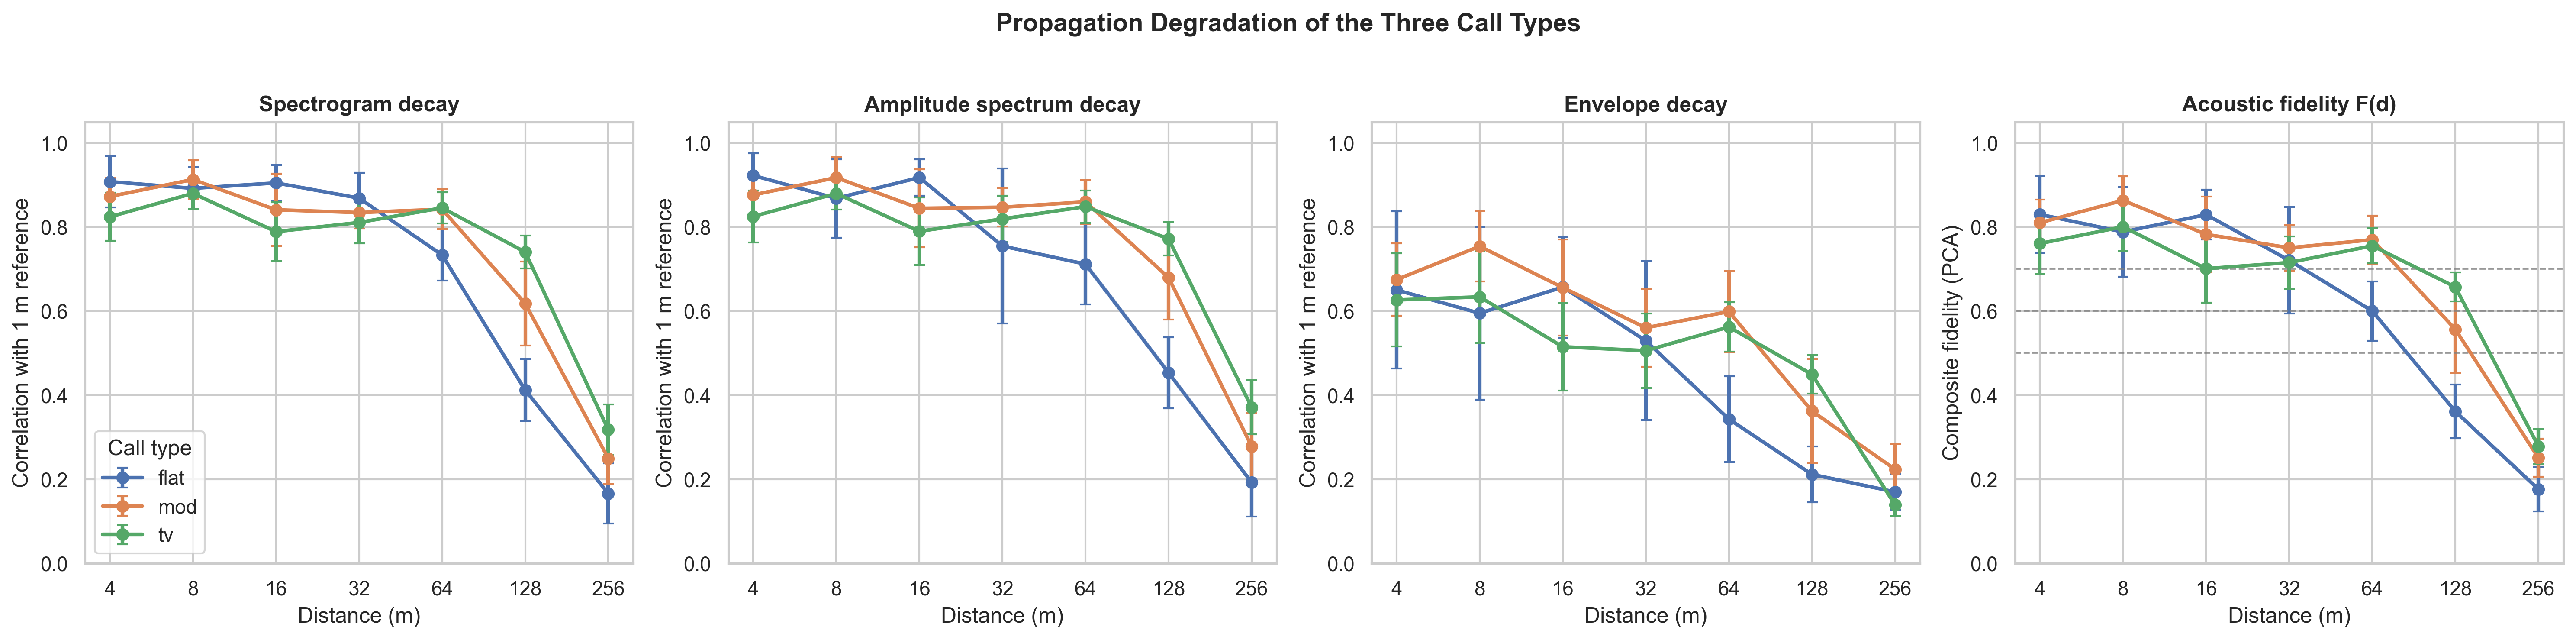
\includegraphics[width=\linewidth,height=.23\textheight,keepaspectratio]{../outputs_p2/P2_fig1_metric_decay.png}\par\smallskip
    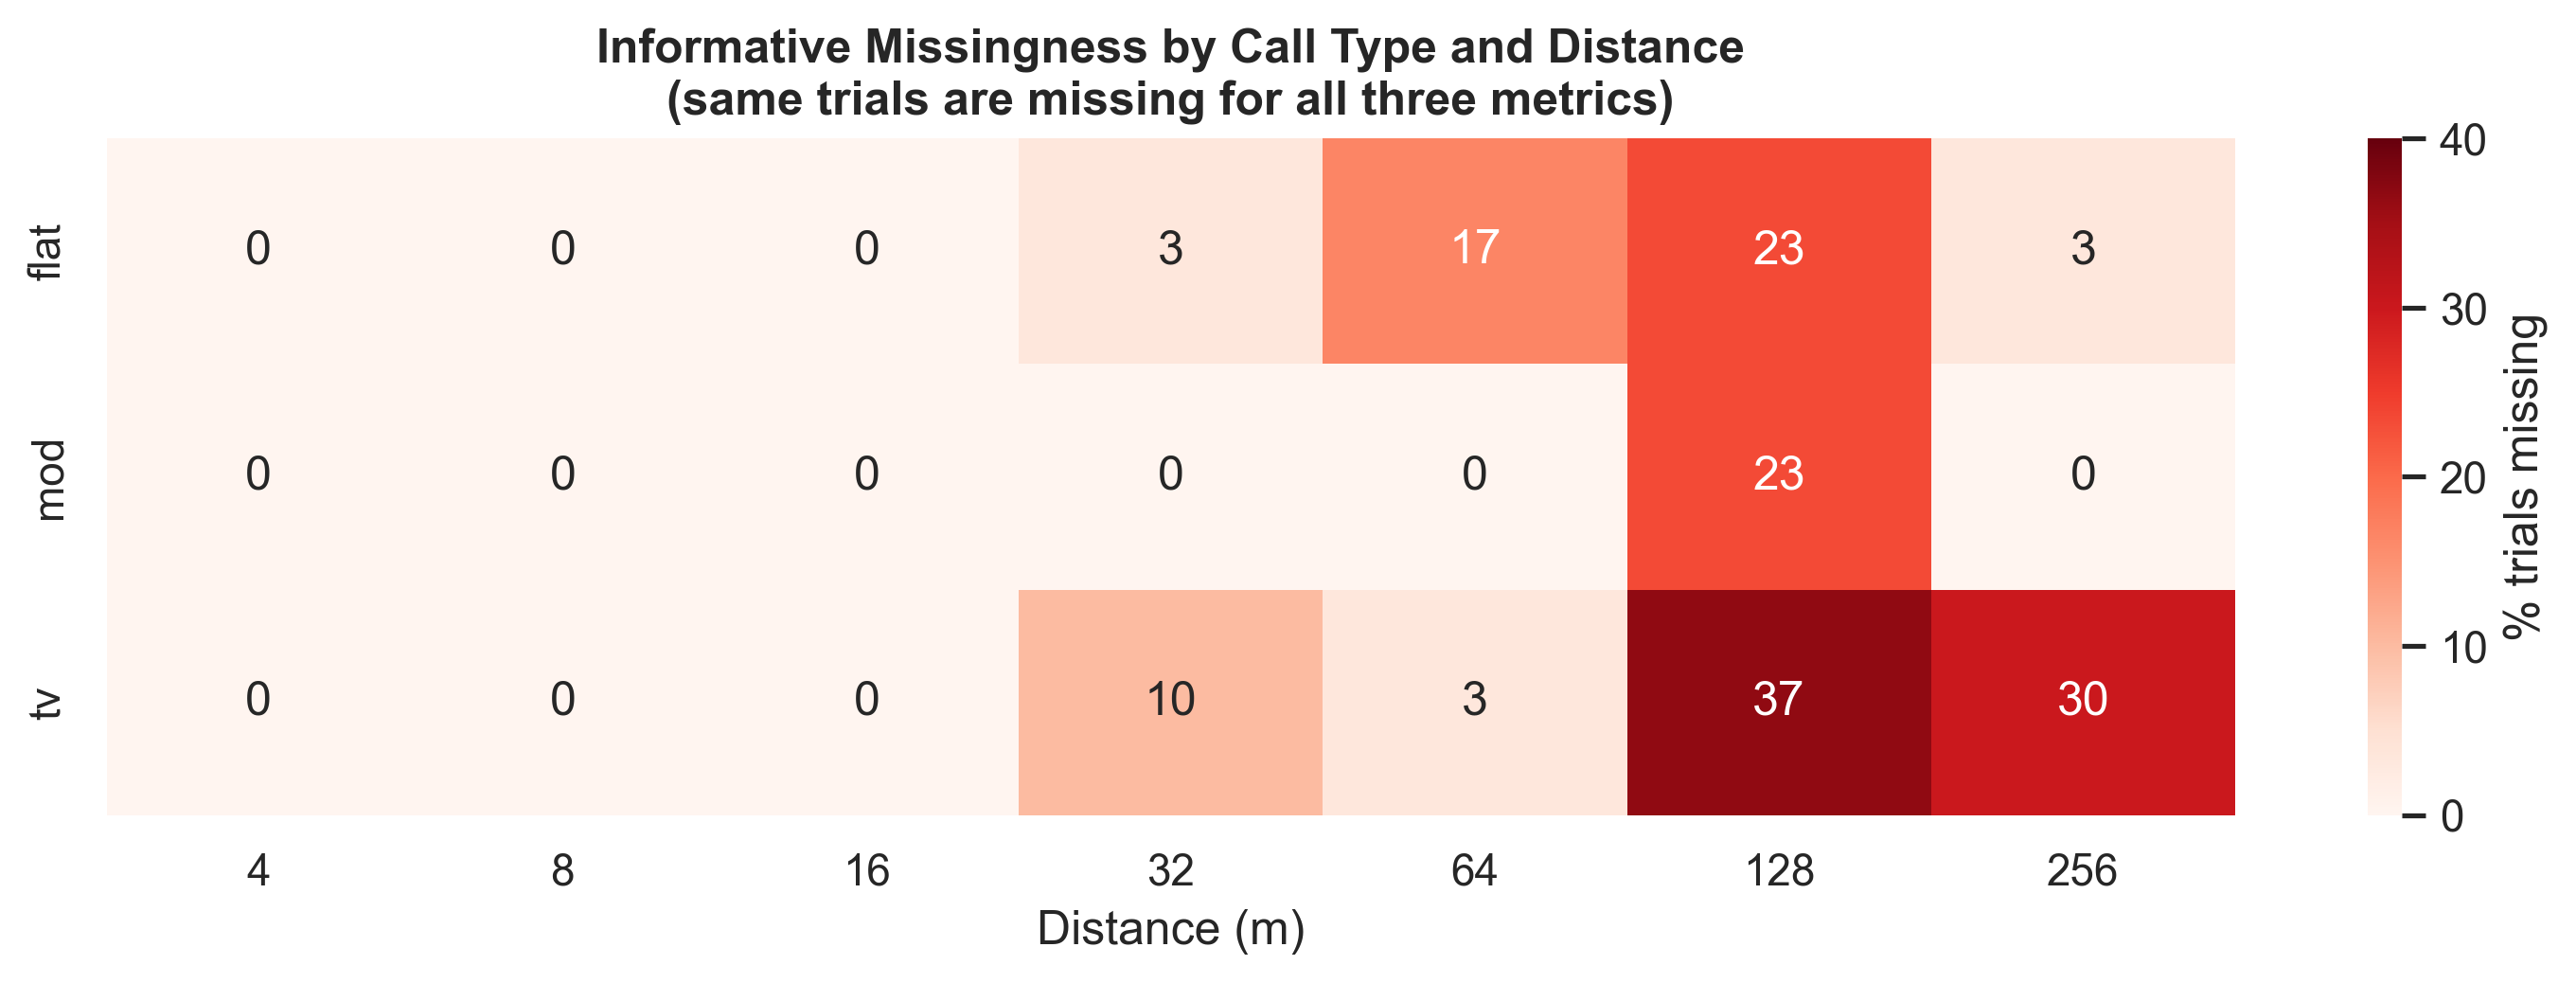
\includegraphics[width=.75\linewidth,height=.20\textheight,keepaspectratio]{../outputs_p2/P2_fig9_missingness.png}
    \caption{三类叫声各指标及 PCA 复合保真度衰减趋势（上）与试次级信息性缺失热图（下）}
    \label{fig:p2_decay_miss}
\end{figure}

\subsection{多模型衰减拟合、试次级交叉验证与模型平均}

\subsubsection{六类候选衰减模型构建}

为兼顾声学传播的物理可解释性与非单调实测数据的拟合稳健性，本文对三类叫声分别构建了涵盖非参数与参数化两类体系的 $6$ 个候选衰减模型：
\begin{enumerate}
    \item \textbf{保序单调回归（Isotonic Regression）}：不预设具体函数形态，仅在观测距离上施加非增单调包络约束以抑制原始均值上跳：
    \begin{equation}
        \min_{\hat{F}} \sum_{i} \bigl(F_i - \hat{F}(d_i)\bigr)^2 \qquad \text{s.t.}\quad \hat{F}(d_1) \ge \hat{F}(d_2) \ge \dots \ge \hat{F}(d_7).
    \end{equation}
    \item \textbf{广义加性样条回归（GAM Spline + RidgeCV）}：以对数距离 $\ln d$ 为自变量构建三次 B 样条基函数 $B_j(\ln d)$，并通过 $L_2$ 岭惩罚（交叉验证选优 $\alpha$）实现平滑拟合：
    \begin{equation}
        F_{\text{GAM}}(d) = \sum_{j=1}^{K} \beta_j B_j(\ln d), \qquad
        \min_{\boldsymbol{\beta}} \sum_{i}\bigl(F_i - F_{\text{GAM}}(d_i)\bigr)^2 + \alpha \|\boldsymbol{\beta}\|_2^2.
    \end{equation}
    \item \textbf{四参数 Logistic 曲线}：有界单调递减曲线，其中 $a, c$ 分别为上下渐近线，$d_0$ 为半衰距离，$b$ 为衰减陡度：
    \begin{equation}
        F_{\text{Logis}}(d) = c + \frac{a - c}{1 + (d / d_0)^b}.
    \end{equation}
    \item \textbf{物理对数--指数衰减模型（Physical log-exp）}：以观测起点 $4\text{ m}$ 重参数化，$b\ln(d/4)$ 表征几何扩散损失，$c(d-4)$ 表征线性介质吸收：
    \begin{equation}
        F_{\text{log-exp}}(d) = F_4 - b\ln\frac{d}{4} - c(d - 4).
    \end{equation}
    \item \textbf{物理幂律--指数衰减模型（Physical power-exp）}：以乘性形式耦合几何扩散幂律项与指数吸收项：
    \begin{equation}
        F_{\text{pow-exp}}(d) = F_4\left(\frac{d}{4}\right)^{-b} e^{-c(d - 4)}.
    \end{equation}
    \item \textbf{Weibull 衰减模型}：常用于刻画加速或减速衰减过程的双参数分布曲线（$\lambda$ 为尺度距离，$k$ 为形状参数）：
    \begin{equation}
        F_{\text{Weib}}(d) = \exp\!\left[-\left(\frac{d}{\lambda}\right)^k\right].
    \end{equation}
\end{enumerate}

\subsubsection{试次级交叉验证与合格模型筛选}

由于同一条录音试次在 $4\text{--}256\text{ m}$ 的 $7$ 个距离上重复观测、存在试次内相关性，常规基于行级样本量的 AIC/BIC 会低估参数不确定性。为此，本文按整条试次（\texttt{TrialID}）划分 $5$ 折交叉验证，以\textbf{试次级交叉验证均方根误差（CV-RMSE）}作为主选优准则：
\begin{equation}
    \text{CV-RMSE}_m = \sqrt{\frac{1}{N_{\text{obs}}}\sum_{f=1}^{5}\sum_{i \in \mathcal{V}_f}\bigl(F_i - \hat{F}_m^{(-f)}(d_i)\bigr)^2},
\end{equation}
其中 $\mathcal{V}_f$ 为第 $f$ 折留出的整条试次观测集合，$\hat{F}_m^{(-f)}$ 为在其余 $4$ 折上训练的第 $m$ 类模型。同时设定严格的\textbf{合格模型筛选门槛}：剔除优化过程中触及参数边界（Boundary=True）的模型，以及拟合较差（$R^2 < 0.60$ 或 $\text{CV-RMSE} > 1.5\min_k \text{CV-RMSE}_k$）的模型。

如表~\ref{tab:p2_models} 所示，筛选结果呈现出鲜明的分化：\textbf{保序回归与 GAM 样条在三类叫声上均表现最优且无参数触界}（CV-RMSE：\texttt{flat} $0.087 / 0.086$、\texttt{mod} $0.069 / 0.068$、\texttt{tv} $0.063 / 0.060$）；而在 \texttt{mod} 与 \texttt{tv} 上，所有参数化物理模型及 Logistic 模型均出现参数触界坍缩，Weibull 呈明显欠拟合（\texttt{tv} 上 $R^2$ 仅 $0.516$），印证了阶段一关于``非单调波动易致刚性参数曲线失真''的诊断。

\begin{table}[htbp]
\centering
\caption{六类信号传播衰减模型试次级 $5$ 折 CV-RMSE、$R^2$ 及模型平均权重对比}
\label{tab:p2_models}
\footnotesize\setlength{\tabcolsep}{3.5pt}
\begin{tabular*}{\linewidth}{@{\extracolsep{\fill}}lccc|ccc|ccc@{}}
\toprule
\multirow{2}{*}{衰减模型} & \multicolumn{3}{c|}{\texttt{flat}} & \multicolumn{3}{c|}{\texttt{mod}} & \multicolumn{3}{c}{\texttt{tv}} \\
 & CV-RMSE & $R^2$ & 权重 & CV-RMSE & $R^2$ & 权重 & CV-RMSE & $R^2$ & 权重 \\
\midrule
\textbf{Isotonic（主模型）} & $0.087$ & $0.881$ & $0.22$ & $0.069$ & $0.893$ & $0.49$ & $0.063$ & $0.850$ & $0.48$ \\
\textbf{GAM spline} & $0.086$ & $0.883$ & $0.22$ & $0.068$ & $0.898$ & $0.51$ & $0.060$ & $0.864$ & $0.52$ \\
Logistic & $0.088$ & $0.878$ & $0.21$ & $0.074^*$ & $0.877$ & $0$ & $0.068^*$ & $0.826$ & $0$ \\
Physical log-exp & $0.096$ & $0.856$ & $0.18$ & $0.076^*$ & $0.871$ & $0$ & $0.082^*$ & $0.748$ & $0$ \\
Physical power-exp & $0.090^*$ & $0.872$ & $0$ & $0.085^*$ & $0.838$ & $0$ & $0.090^*$ & $0.694$ & $0$ \\
Weibull & $0.102$ & $0.838$ & $0.16$ & $0.105^\dagger$ & $0.752$ & $0$ & $0.113^\dagger$ & $0.516$ & $0$ \\
\bottomrule
\end{tabular*}
\par\smallskip{\scriptsize\raggedright 注：$^*$ 表示优化触及参数边界（Boundary=True）；$^\dagger$ 表示拟合较差（PoorFit=True）；均不纳入合格模型平均。\par}
\end{table}

\subsubsection{稳健主模型确立与合格模型平均}

综合预测精度与物理单调性要求，本文确立\textbf{保序单调回归（Isotonic Regression）}为稳健主模型（GAM 样条在个别距段可能局部微升，而保序包络严格保证随距离非增，便于唯一反解有效通信距离）。为进一步刻画模型选择不确定性，对通过筛选的合格模型集合 $\mathcal{M}_{\text{elig}}$ 按反误差平方加权构建\textbf{模型平均曲线}：
\begin{equation}\label{eq:p2_model_average}
    F_{\text{avg}}(d) = \sum_{m \in \mathcal{M}_{\text{elig}}} \omega_m \hat{F}_m(d), \qquad
    \omega_m = \frac{\text{CV-RMSE}_m^{-2}}{\sum_{k \in \mathcal{M}_{\text{elig}}} \text{CV-RMSE}_k^{-2}}.
\end{equation}
最终在 \texttt{mod}（Isotonic $0.49$、GAM $0.51$）与 \texttt{tv}（$0.48 / 0.52$）上由两类非参数模型均分权重，在 \texttt{flat} 上由 $5$ 个合格模型共同加权（拟合对比见图~\ref{fig:p2_fit}）。

\begin{figure}[htbp]
    \centering
    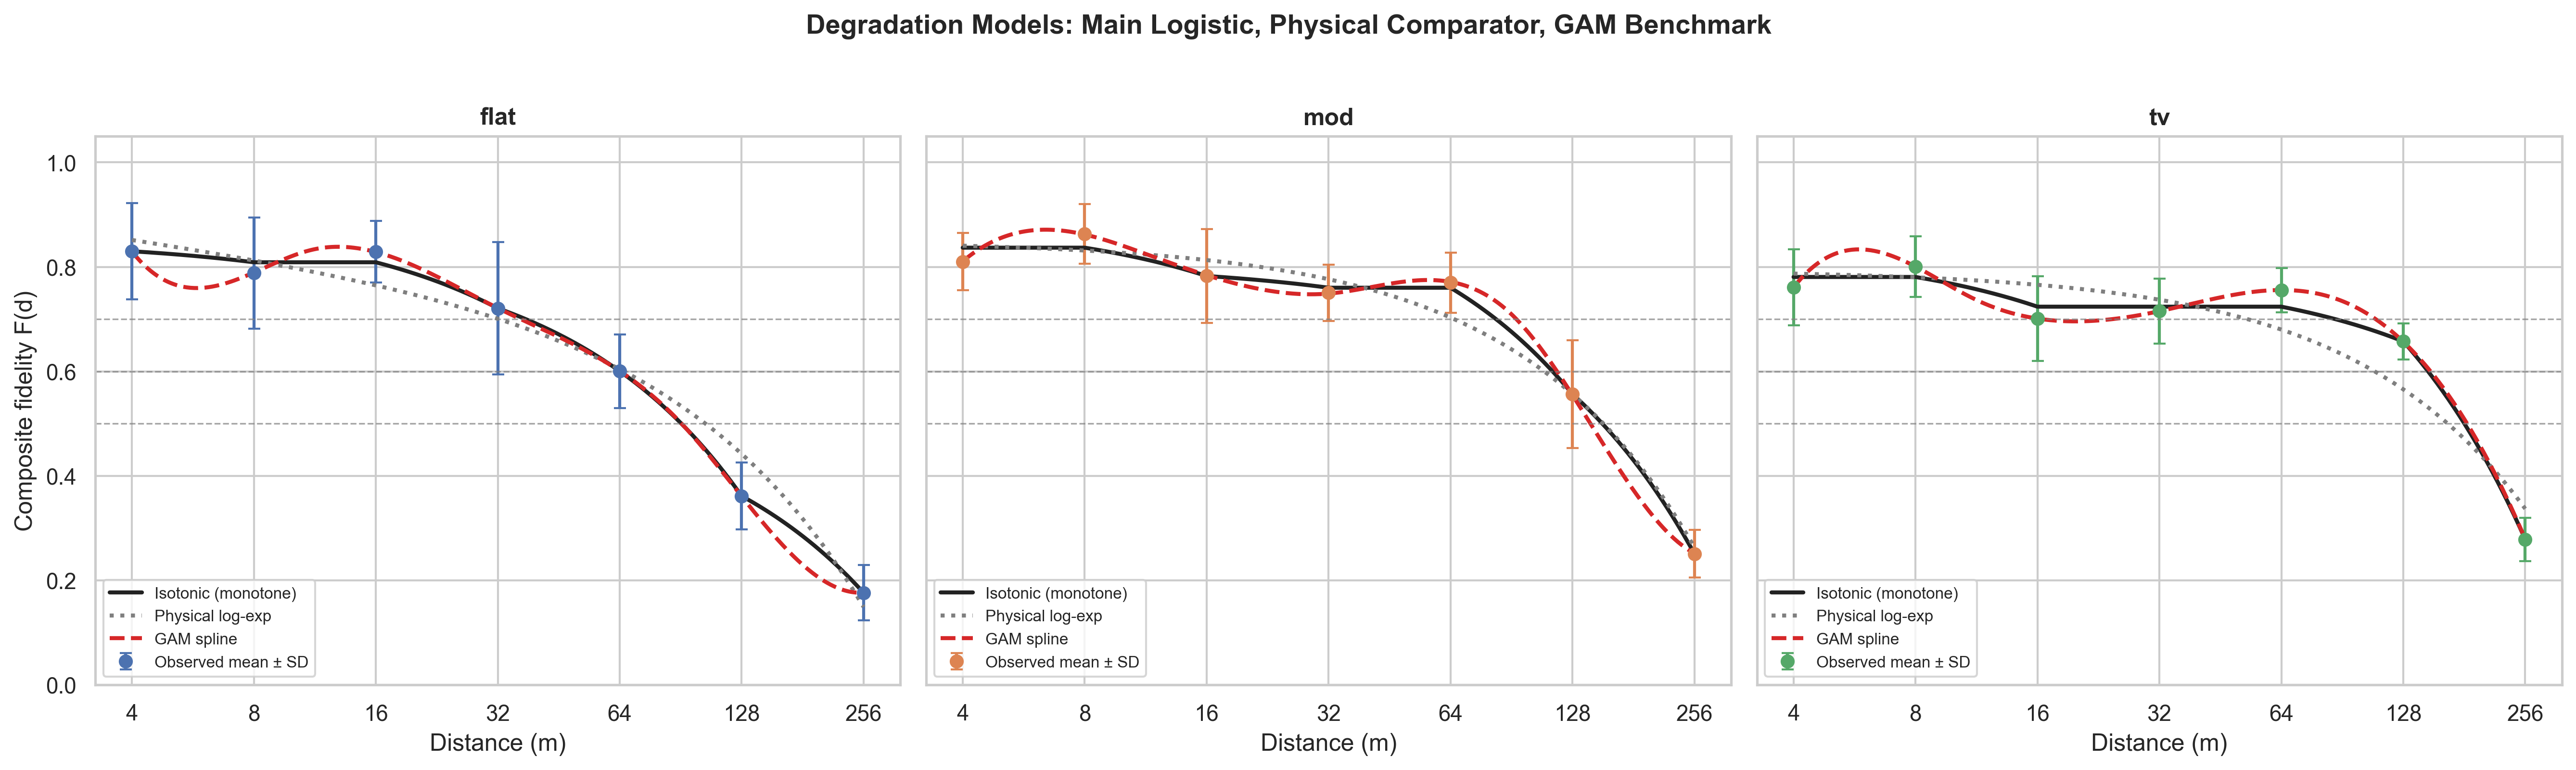
\includegraphics[width=\linewidth,height=.24\textheight,keepaspectratio]{../outputs_p2/P2_fig2_model_fits.png}
    \caption{三类叫声主保序模型、物理对数--指数模型与 GAM 样条拟合曲线对比}
    \label{fig:p2_fit}
\end{figure}


\subsection{分级识别阈值设计与双视角有效通信距离估计}

针对题目要求企鹅能否识别叫声取决于传播后的相似度是否达到阈值，本文设计三级识别阈值：\textbf{潜在识别 $\tau = 0.50$}（最低可探测边界）、\textbf{一般识别 $\tau = 0.60$}（中等清晰度）
与\textbf{可靠识别 $\tau = 0.70$}（高保真稳定辨识）。

为区分``群体平均可达距离''与``个体试次保障距离''，本文从双重视角求解有效距离：
（1）\textbf{群体均值有效距离 $d_\tau$}：反解 $\hat{F}(d_\tau) = \tau$，通过试次自助法（$N_{\text{boot}} = 1000$，每次重抽样同步重估 PCA 权重）给出 $95\%$ CI 及合格模型平均区间；
（2）\textbf{个体概率有效距离 $R_\tau(p)$}：基于全部 $7$ 个距离均有效的共同试次（\texttt{flat}/\texttt{mod} $N=230$，\texttt{tv} $N=180$）拟合单调 Logistic 概率模型并配套非参数经验交叉区间（Bracket）：
\begin{equation}\label{eq:p2_probability_range}
    R_\tau(p) = \max\bigl\{d : P(F(d) \ge \tau) \ge p\bigr\}, \qquad
    \operatorname{logit}\,P(F \ge \tau \mid d) = a + b\ln d \quad (b \le 0).
\end{equation}

表~\ref{tab:p2_ranges} 与图~\ref{fig:p2_range_prob} 汇总了两大核心标准（$\tau = 0.50$ 与 $\tau = 0.70$）下的双视角测距结果：潜在识别（$\tau = 0.50$）
下模型平均距离依次为 \texttt{tv} $182.6\text{ m}$、\texttt{mod} $145.5\text{ m}$、\texttt{flat} $89.7\text{ m}$；可靠识别（$\tau = 0.70$）
下缩短至 \texttt{tv} $102.2\text{ m}$、\texttt{mod} $88.4\text{ m}$、\texttt{flat} $35.5\text{ m}$。若要求 $p = 0.90$ 的个体试次均达可靠识别，
距离被压至近源区（\texttt{flat} $8.6\text{ m}$、\texttt{mod} $[8, 16]\text{ m}$、\texttt{tv} $4.3\text{ m}$）

综上说明，$p = 0.50/0.75$ 宜作主生态通信半径，$p = 0.90$ 宜作严苛个体下界。

\begin{table}[htbp]
\centering
\caption{三类叫声在潜在识别（$\tau=0.50$）与可靠识别（$\tau=0.70$）下的有效通信距离汇总（单位：$\text{m}$）}
\label{tab:p2_ranges}
\footnotesize\setlength{\tabcolsep}{2pt}
\begin{tabular*}{\linewidth}{@{\extracolsep{\fill}}lcccccc@{}}
\toprule
叫声 & 阈值 $\tau$ & \shortstack{主保序均值\\[1pt]$[95\%\text{ CI}]$} & \shortstack{模型平均\\[1pt]$[\text{合格区间}]$} & \shortstack{$R_\tau(0.50)$\\[1pt]$[\text{经验区间}]$} & \shortstack{$R_\tau(0.75)$\\[1pt]$[\text{经验区间}]$} & \shortstack{$R_\tau(0.90)$\\[1pt]$[\text{经验区间}]$} \\
\midrule
\texttt{flat} & $0.50$ & \shortstack{$90.9$\\[1pt]$[89.1, 92.9]$} & \shortstack{$89.7$\\[1pt]$[77.7, 104.1]$} & \shortstack{$84.4$\\[1pt]$[64, 128]$} & \shortstack{$66.1$\\[1pt]$[64, 128]$} & \shortstack{$51.8$\\[1pt]$[32, 64]$} \\
\texttt{mod} & $0.50$ & \shortstack{$151.6$\\[1pt]$[146.3, 156.3]$} & \shortstack{$145.5$\\[1pt]$[141.7, 151.6]$} & \shortstack{$138.7$\\[1pt]$[128, 256]$} & \shortstack{$105.7$\\[1pt]$[64, 128]$} & \shortstack{$80.7$\\[1pt]$[64, 128]$} \\
\texttt{tv} & $0.50$ & \shortstack{$181.1$\\[1pt]$[179.5, 182.0]$} & \shortstack{$182.6$\\[1pt]$[181.1, 183.9]$} & \shortstack{$179.3$\\[1pt]$[128, 256]$} & \shortstack{$134.8$\\[1pt]$[128, 256]$} & \shortstack{$101.4^*$\\[1pt]$[128, 256]$} \\
\midrule
\texttt{flat} & $0.70$ & \shortstack{$37.5$\\[1pt]$[33.8, 40.9]$} & \shortstack{$35.5$\\[1pt]$[28.8, 40.8]$} & \shortstack{$28.3^*$\\[1pt]$[32, 64]$} & \shortstack{$15.6$\\[1pt]$[4, 32]$} & \shortstack{$8.6$\\[1pt]$[4, 32]$} \\
\texttt{mod} & $0.70$ & \shortstack{$82.9$\\[1pt]$[80.8, 85.1]$} & \shortstack{$88.4$\\[1pt]$[82.9, 93.0]$} & \shortstack{$61.3^*$\\[1pt]$[64, 128]$} & \shortstack{$31.7^*$\\[1pt]$[64, 128]$} & \shortstack{$16.4^*$\\[1pt]$[8, 16]$} \\
\texttt{tv} & $0.70$ & \shortstack{$86.9$\\[1pt]$[81.7, 89.3]$} & \shortstack{$102.2$\\[1pt]$[86.9, 109.4]$} & \shortstack{$45.0$\\[1pt]$[8, 128]$} & \shortstack{$13.9$\\[1pt]$[8, 128]$} & \shortstack{$4.3$\\[1pt]$[4, 128]$} \\
\bottomrule
\end{tabular*}
\par\smallskip{\scriptsize\raggedright 注：一般识别（$\tau=0.60$）主保序均值依次为 \texttt{flat} $64.1\text{ m}$、\texttt{mod} $114.3\text{ m}$、\texttt{tv} $147.4\text{ m}$；$^*$ 表示光滑插值点落在经验区间外，以经验区间为准。\par}
\end{table}

\begin{figure}[htbp]
    \centering
    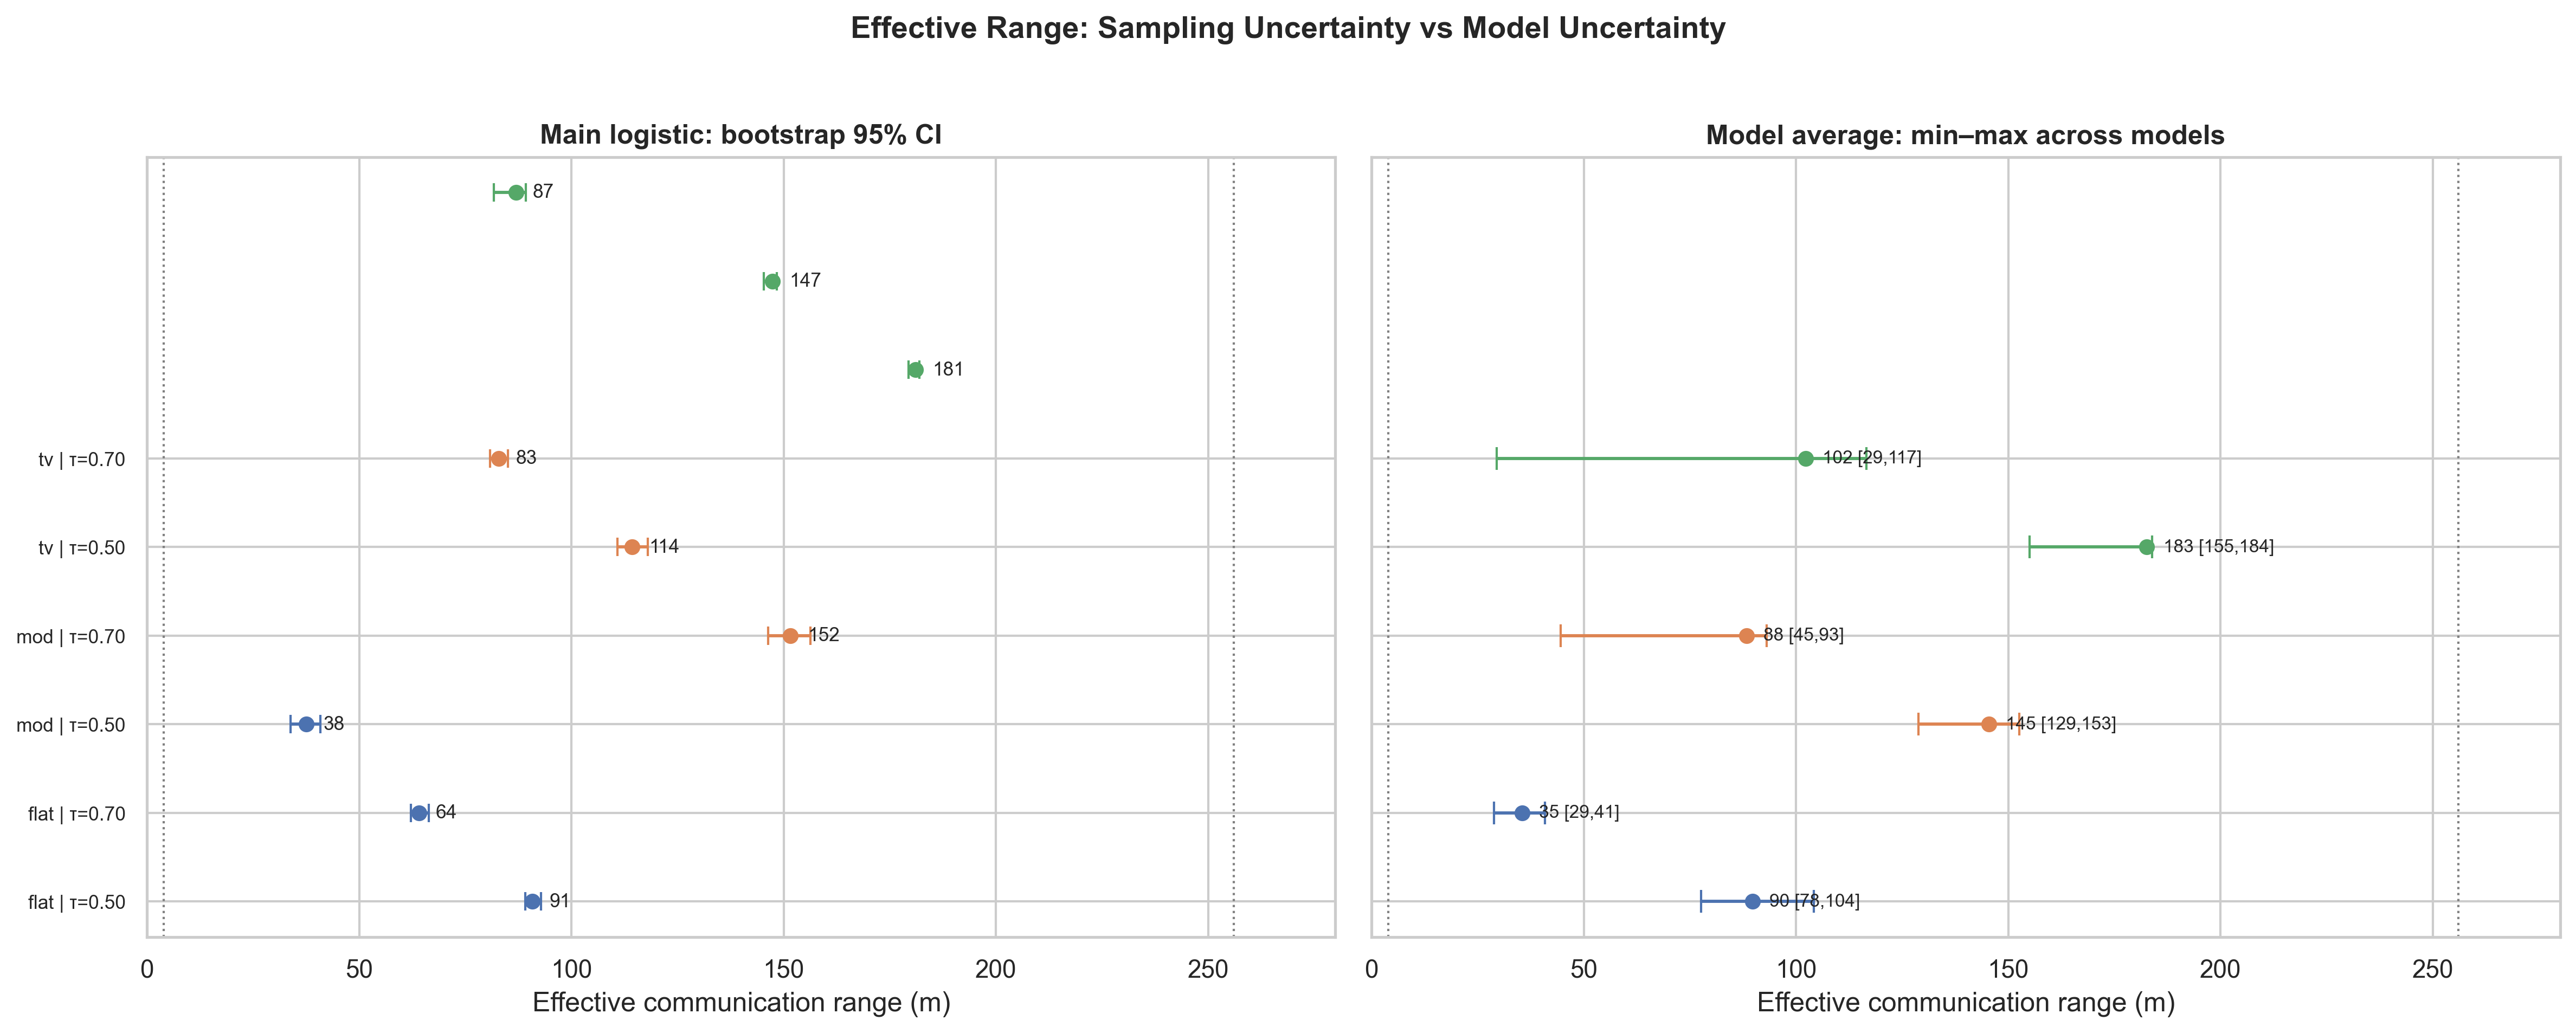
\includegraphics[width=\linewidth,height=.23\textheight,keepaspectratio]{../outputs_p2/P2_fig3_effective_range.png}\par\smallskip
    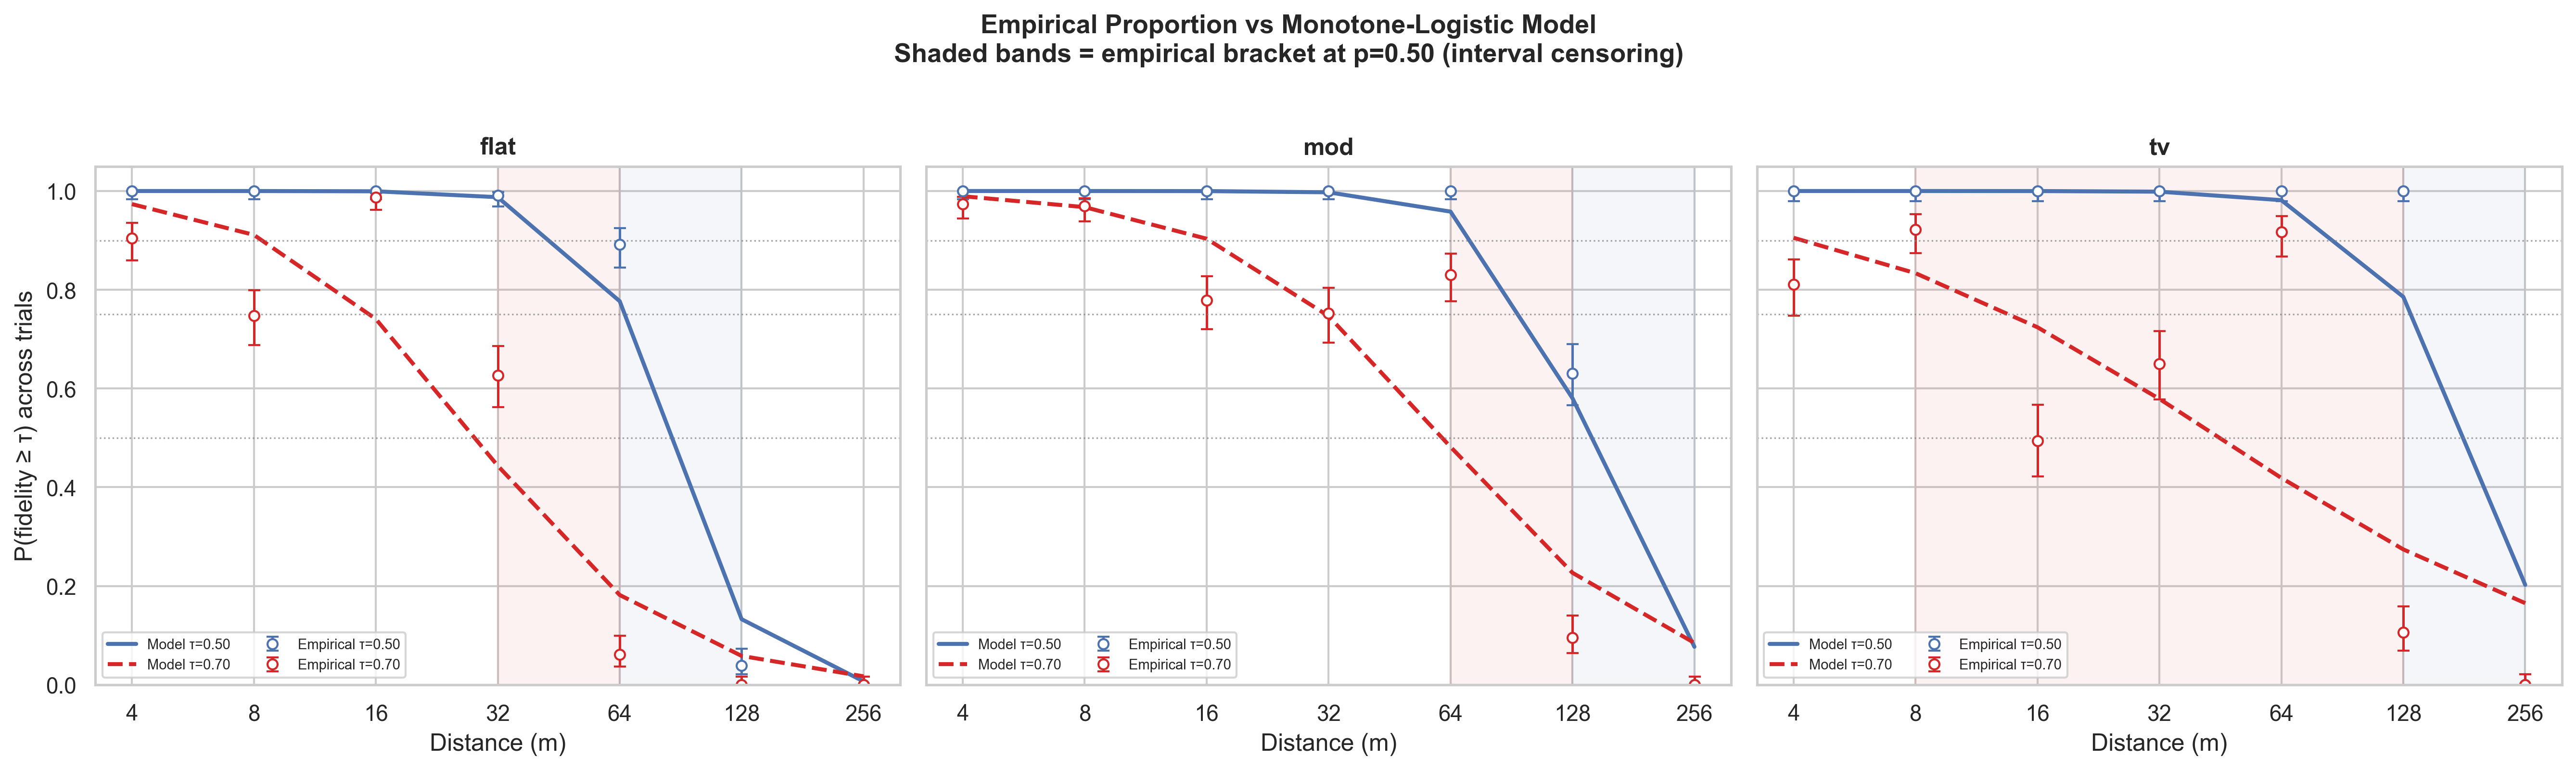
\includegraphics[width=\linewidth,height=.23\textheight,keepaspectratio]{../outputs_p2/P2_fig11_recognition_probability.png}
    \caption{抽样自助法 CI 与模型离散区间对比（上）及共同试次个体识别概率曲线与经验区间（下）}
    \label{fig:p2_range_prob}
\end{figure}

\FloatBarrier

\subsection{多维敏感性分析、不确定性分解与远距离稳健性评判}

我们进一步开展敏感性分析与龙卷风不确定性分解，系统评估各类误差源对结论的影响。

\subsubsection{阈值敏感性与 \texttt{tv}--\texttt{mod} 交叉点}

扫描 $\tau \in [0.40, 0.80]$ 显示（见图~\ref{fig:p2_threshold_sens}），\texttt{tv} 与 \texttt{mod} 的保序曲线在 $\tau^* = 0.706\,[0.697, 0.713]$（$R^* = 80.9\,[77.3, 85.4]\text{ m}$）处相交；加权保序回归与 GAM 节点数（$k=4,5,6$）检验表明主趋势稳定。

\begin{figure}[H]
    \centering
    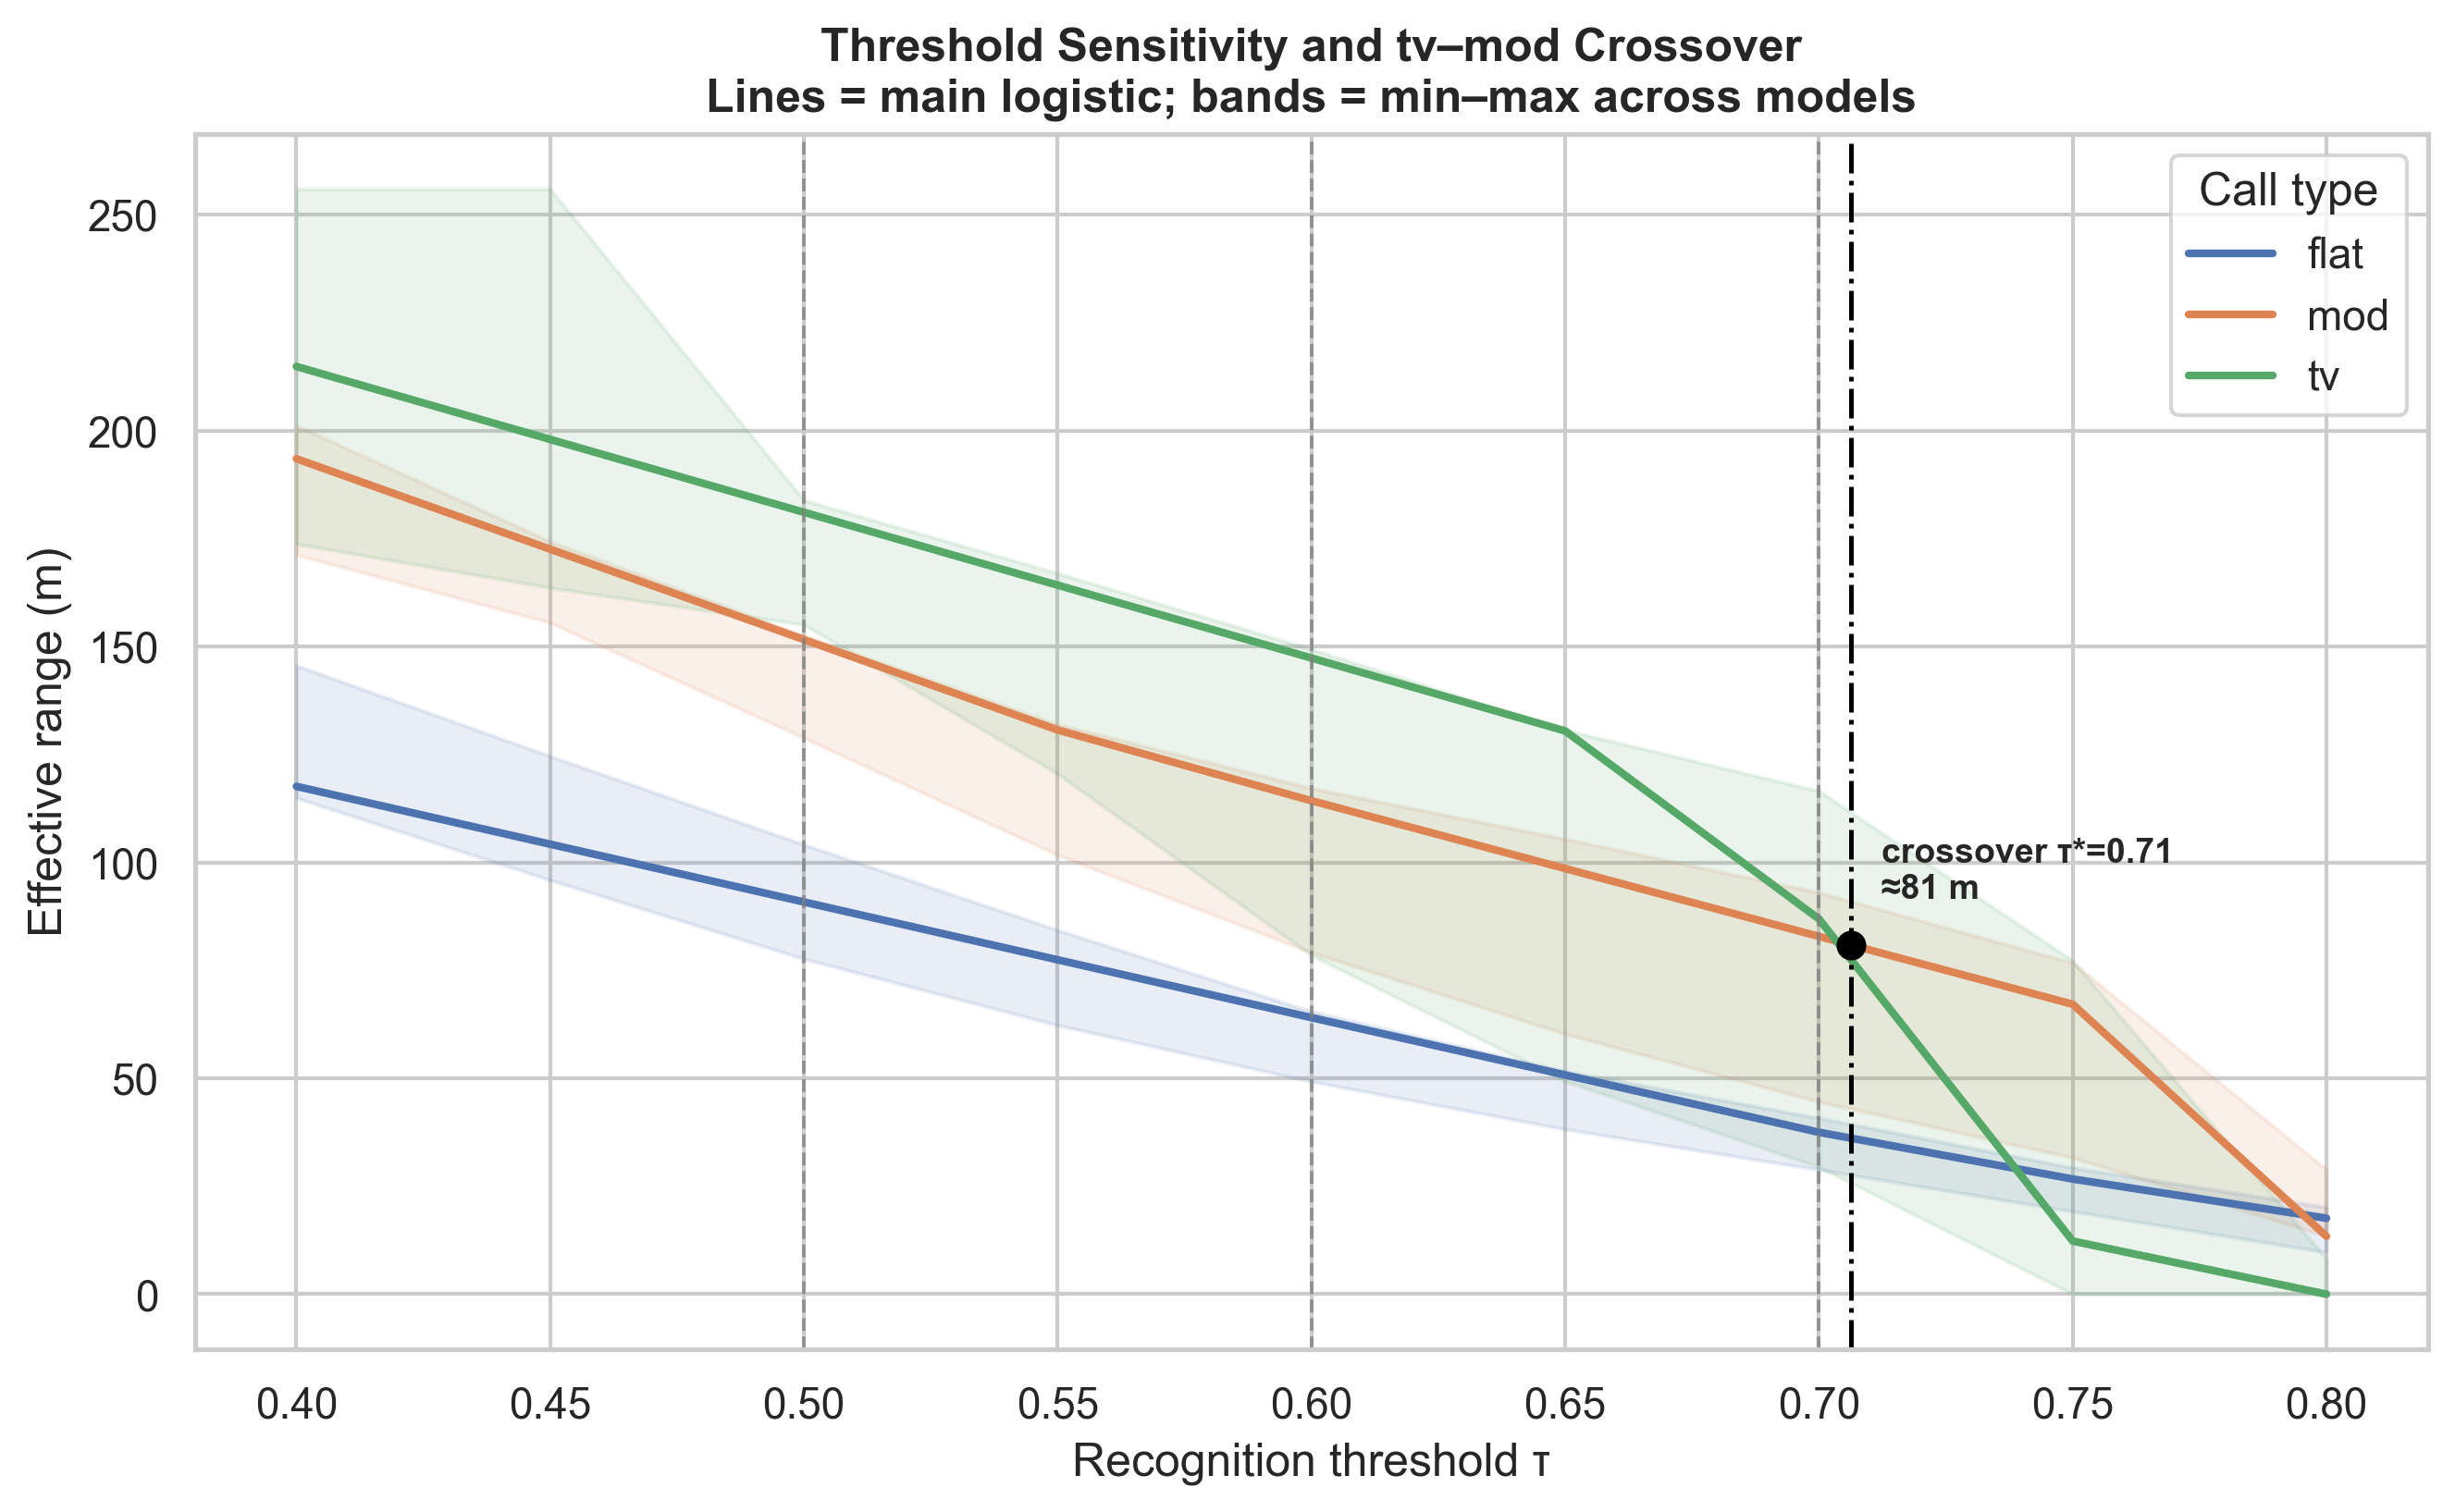
\includegraphics[width=\linewidth,height=.24\textheight,keepaspectratio]{../outputs_p2/P2_fig4_threshold_sensitivity.png}
    \caption{识别阈值与有效距离的关系及 \texttt{tv} 与 \texttt{mod} 的交叉点}\label{fig:p2_threshold_sens}
\end{figure}

\subsubsection{信息性缺失部分识别边界（MNAR Bounds）}

将缺失试次按最差（$F=0$）与最优（$F=1$）填补重跑保序模型（见图~\ref{fig:p2_missing_bounds}）。在 $\tau = 0.70$ 下，\texttt{flat}（$[31.5, 47.2]\text{ m}$）与 \texttt{mod}（$[75.5, 102.4]\text{ m}$）均有可靠边界（$R^2 \ge 0.65$）；而 \texttt{tv} 因远距离缺失严重，最差（$17.1\text{ m}, R^2=0.581$）与最优（$152.2\text{ m}, R^2=0.262$）拟合均不可靠，表明 \texttt{tv} 在非随机缺失下\textbf{不可识别}，完全样本估计偏乐观。

\begin{figure}[H]
    \centering
    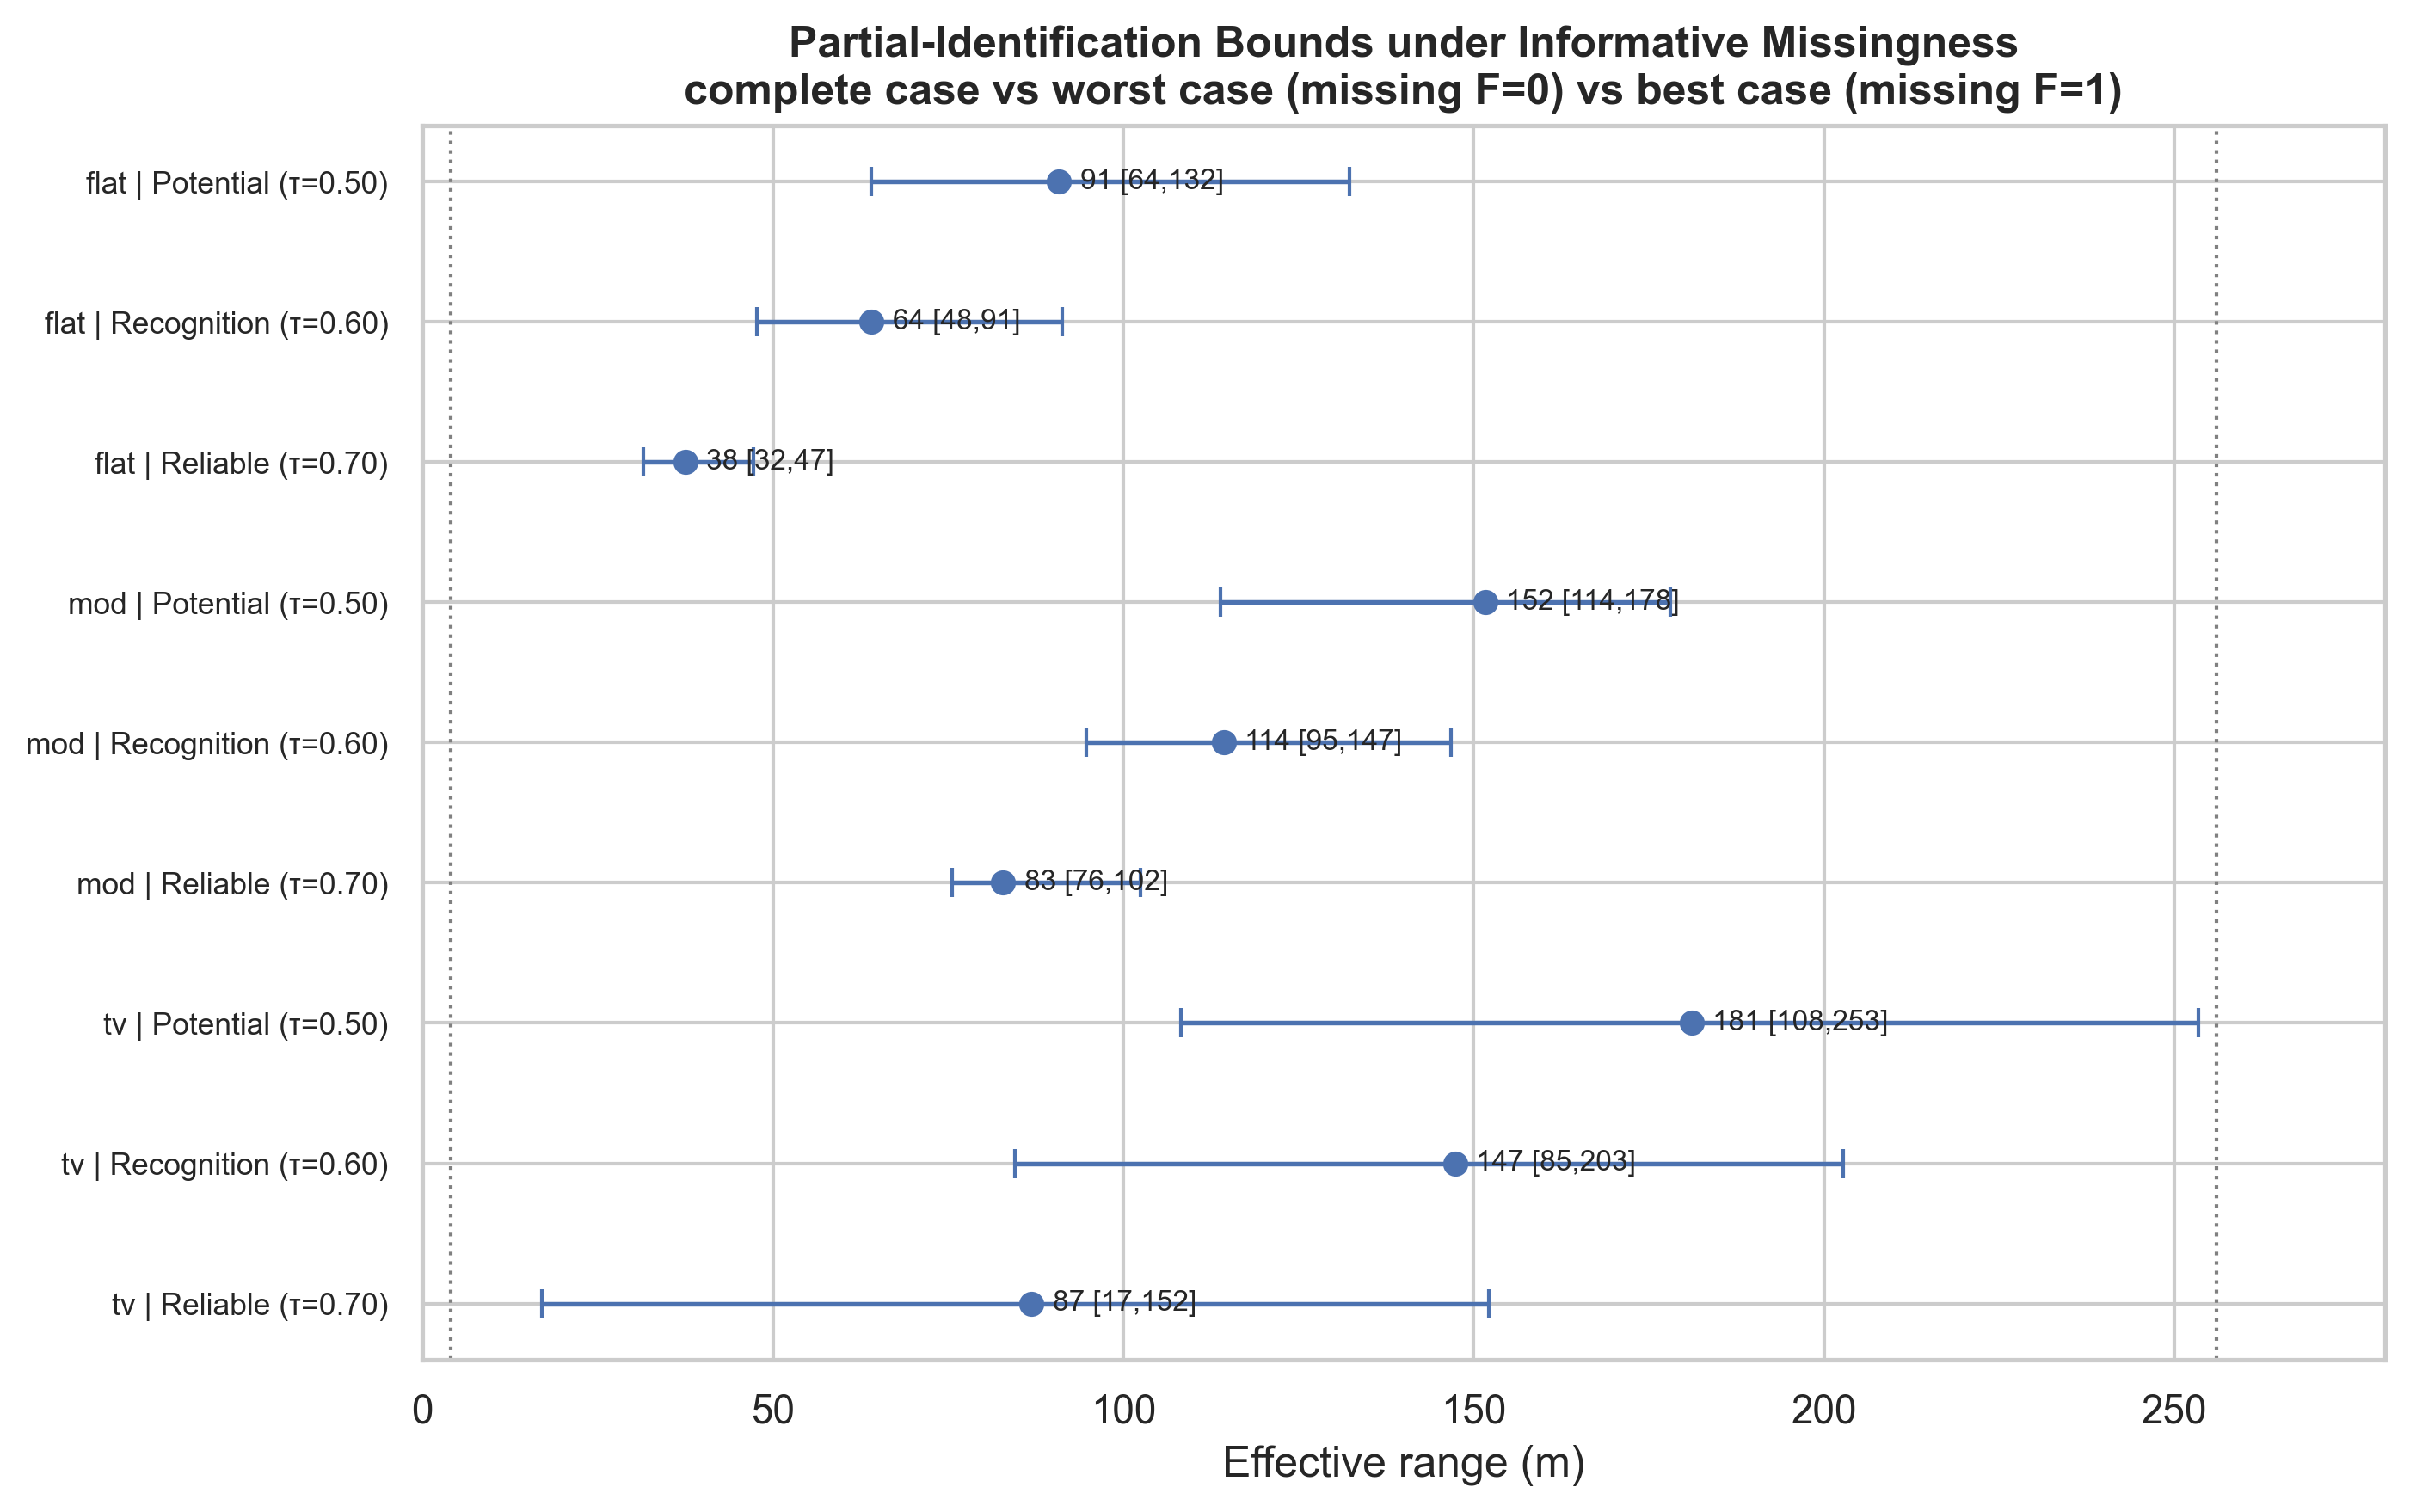
\includegraphics[width=\linewidth,height=.24\textheight,keepaspectratio]{../outputs_p2/P2_fig10_missingness_bounds.png}
    \caption{最差与最优缺失情景下有效距离的部分识别边界}\label{fig:p2_missing_bounds}
\end{figure}

\subsubsection{单通道短板与融合权重敏感性}

单指标测距结果见图~\ref{fig:p2_channel_ranges}。在 $\tau=0.70$ 下语谱图与振幅谱有效距离远高于综合值（\texttt{tv} 达 $140 / 151\text{ m}$），但\textbf{振幅包络通道}在 \texttt{flat} 与 \texttt{tv} 于 $4\text{ m}$ 处即未达 $0.70$（\texttt{mod} 仅 $10\text{ m}$），说明综合 $d_{70}$ 属于频谱通道补偿后的均值。

\begin{figure}[H]
    \centering
    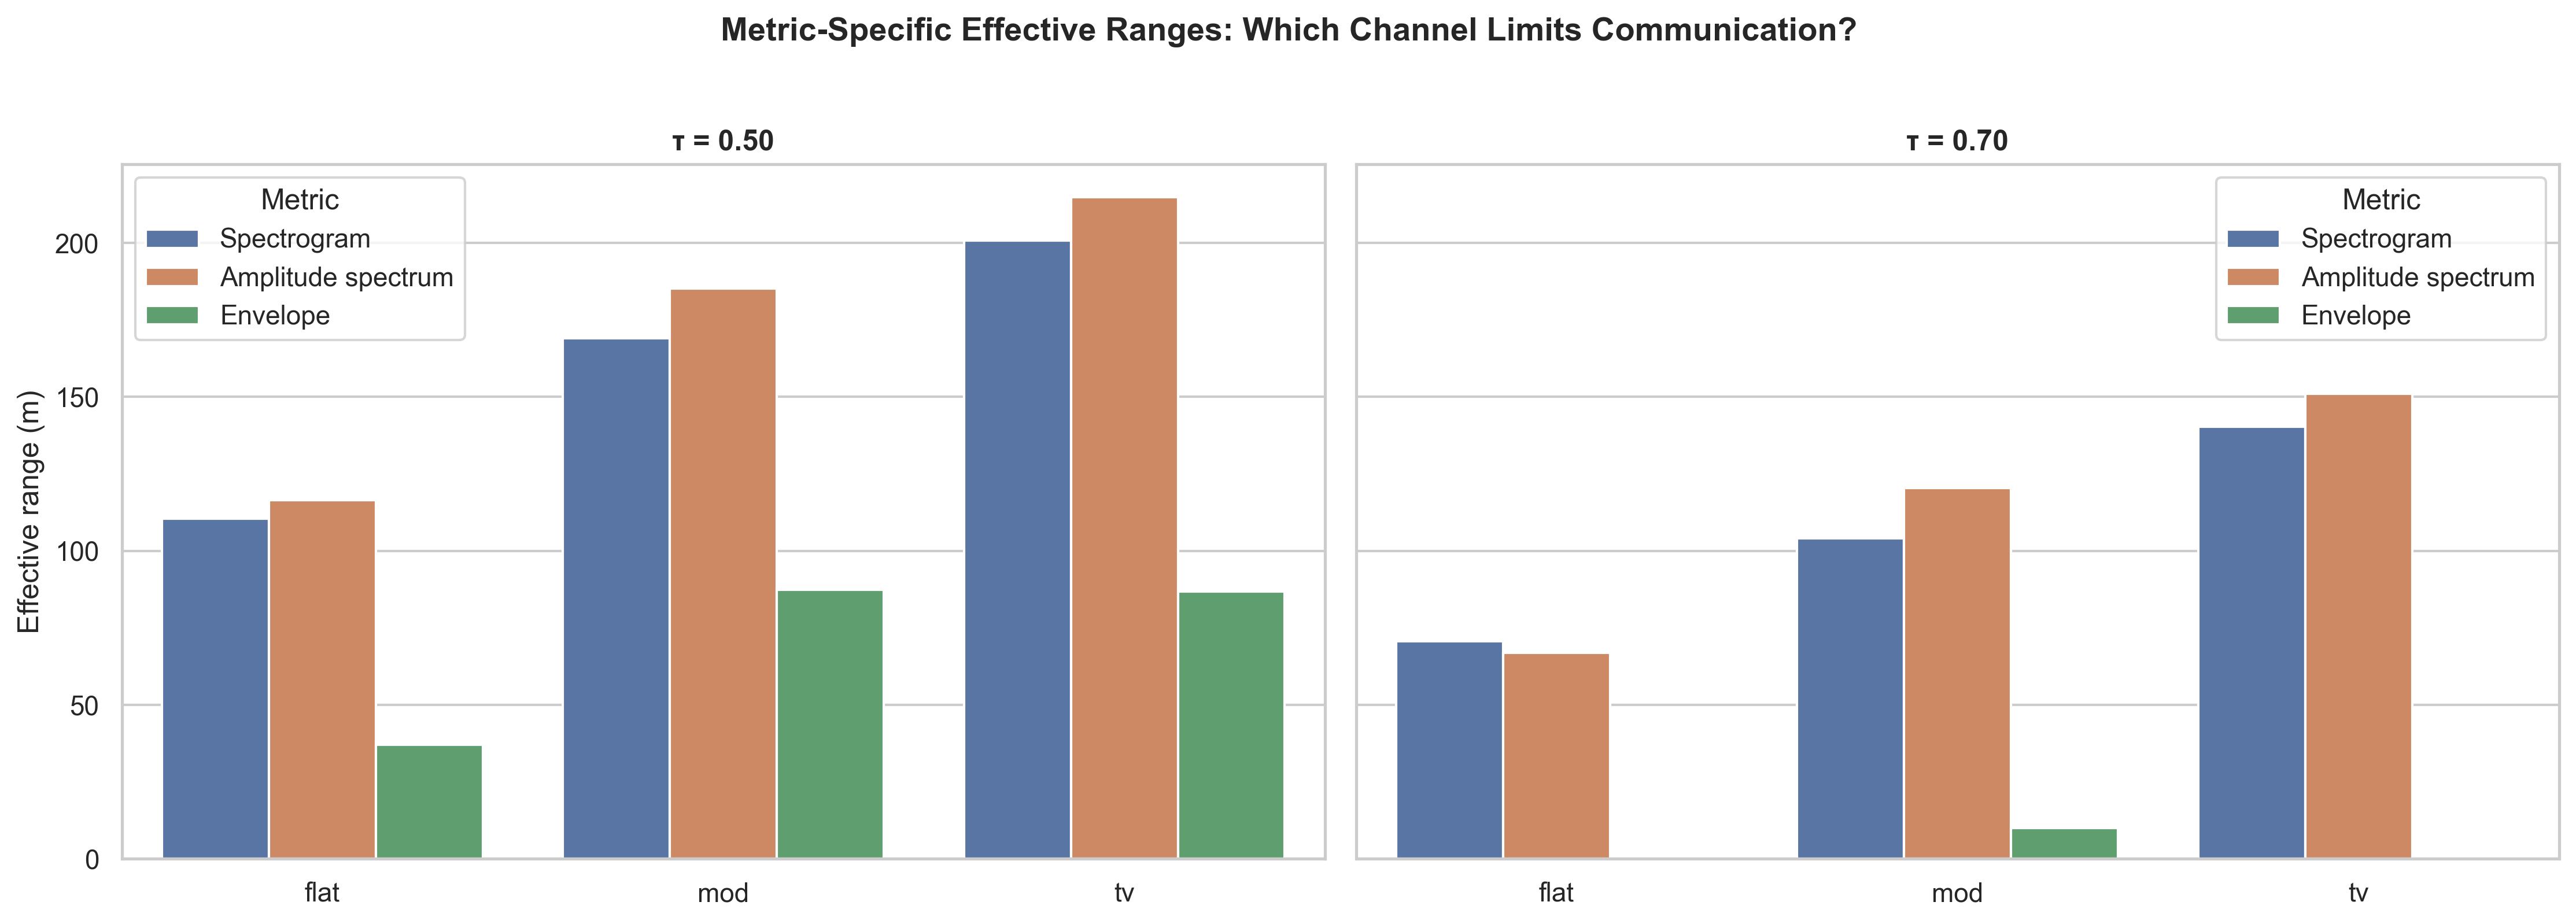
\includegraphics[width=\linewidth,height=.23\textheight,keepaspectratio]{../outputs_p2/P2_fig12_metric_specific_ranges.png}
    \caption{不同识别阈值下各声学通道的有效距离}\label{fig:p2_channel_ranges}
\end{figure}

\Needspace{.36\textheight}
图~\ref{fig:p2_fusion_sens} 比较了各融合方法。换用对弱通道更敏感的熵权法或几何平均后，\texttt{tv} 的 $d_{70}$ 从 PCA 的 $86.9\text{ m}$ 骤降至 $14.8\text{ m}$（熵权）与 $71.9\text{ m}$（几何），而 \texttt{mod}（$73.0\text{--}82.9\text{ m}$）明显更稳健。

\begin{figure}[H]
    \centering
    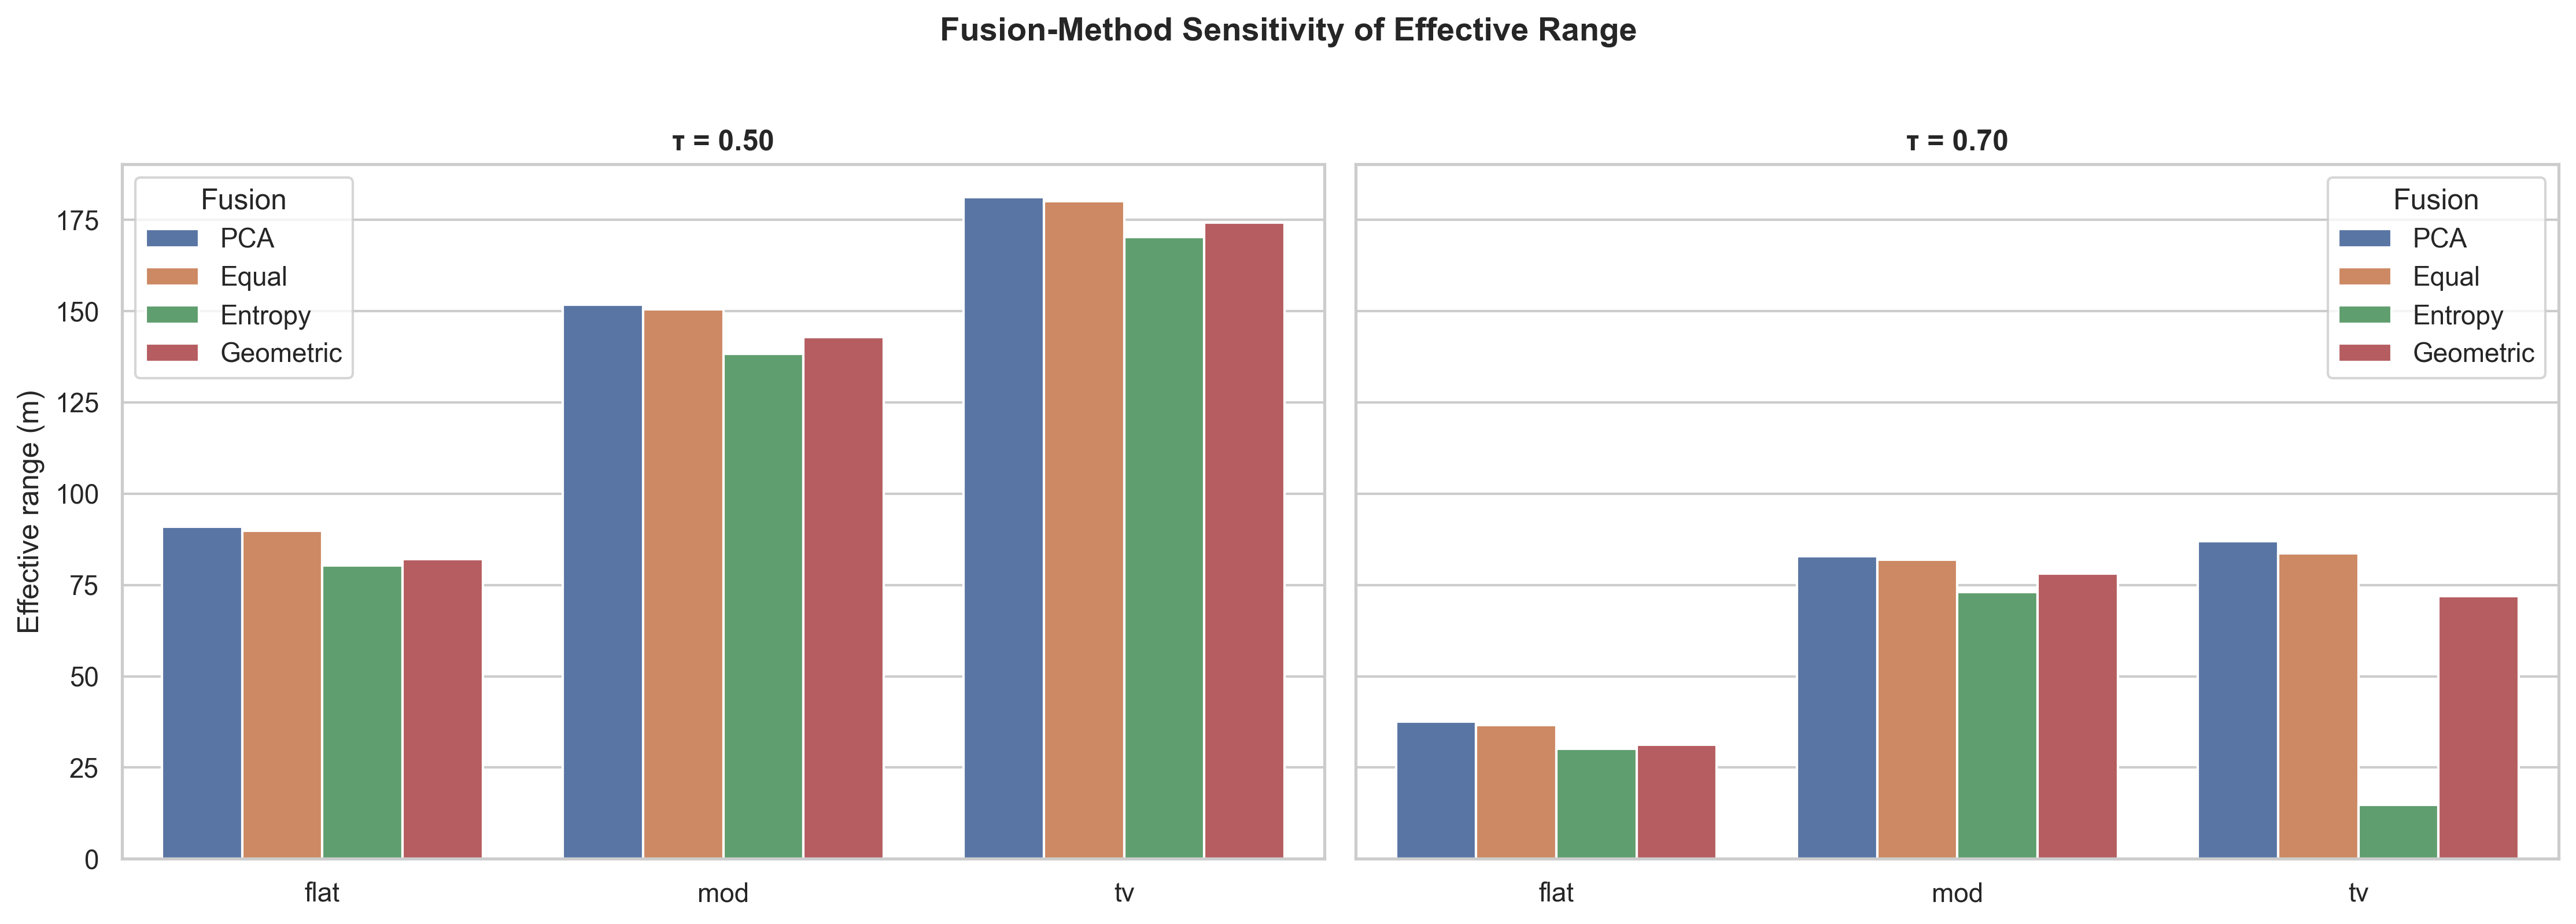
\includegraphics[width=\linewidth,height=.23\textheight,keepaspectratio]{../outputs_p2/P2_fig8_fusion_sensitivity.png}
    \caption{不同融合方法对有效距离估计的影响}\label{fig:p2_fusion_sens}
\end{figure}

\subsubsection{龙卷风不确定性分解（$\tau = 0.70$）}

如图~\ref{fig:p2_tornado} 所示，抽样自助法 CI 极窄（$4.3\text{--}7.6\text{ m}$），真正主导不确定性的是\textbf{阈值扰动 $\pm 0.05$}（\texttt{flat} $24.1\text{ m}$、\texttt{mod} $31.4\text{ m}$、\texttt{tv} 达 $118.2\text{ m}$）、\textbf{融合方法}（\texttt{tv} $72.1\text{ m}$）与\textbf{缺失机制}（\texttt{mod} $26.9\text{ m}$，\texttt{tv} 不可识别）。

\begin{figure}[H]
    \centering
    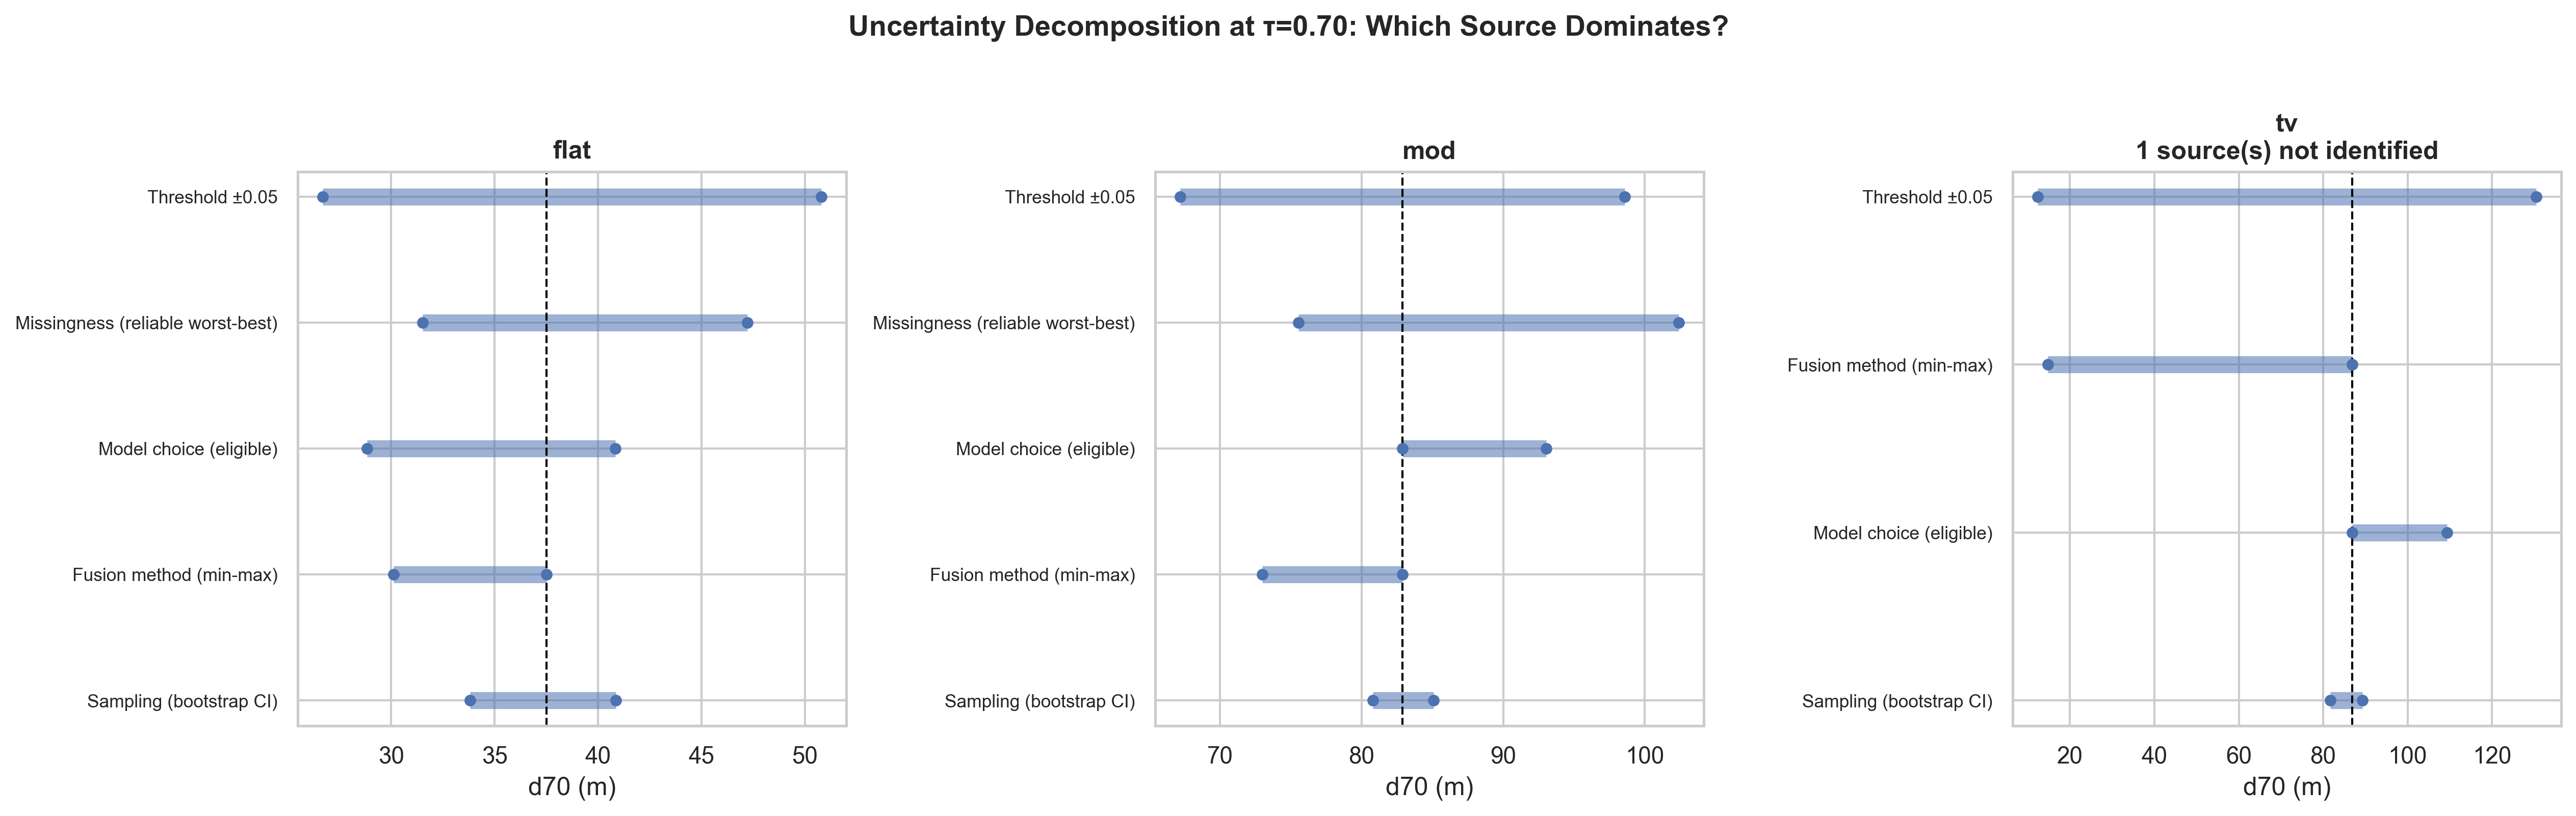
\includegraphics[width=\linewidth,height=.24\textheight,keepaspectratio]{../outputs_p2/P2_fig15_tornado.png}
    \caption{$\tau=0.70$ 下五类不确定性来源的区间宽度}\label{fig:p2_tornado}
\end{figure}

\Needspace{.60\textheight}
\subsubsection{远距离传播稳健性综合结论}

结合两两差值自助法检验与对数距离积分面积 
$\text{AUC}_{\log} = \frac{1}{\ln(256/4)}\int_{4}^{256} F_{\text{avg}}(d)\,\mathrm{d}(\ln d)$（\texttt{mod} $= 0.713$、\texttt{tv} $= 0.699$、\texttt{flat} $= 0.637$），结合图~\ref{fig:p2_robustness} 
得出分情景结论：（1）在\textbf{潜在识别标准（$\tau = 0.50$）}下，\texttt{tv} 明确最优（模型平均 $182.6\text{ m}$，相对 \texttt{mod} 差值 $+29.3\,[24.7, 34.3]\text{ m}$，$P=1.000$），
其次为 \texttt{mod}（$145.5\text{ m}$），\texttt{flat}（$89.7\text{ m}$）最弱；（2）在\textbf{可靠识别标准（$\tau = 0.70$）}下，\texttt{flat}（$35.5\text{ m}$）显著最低；
而 \texttt{tv}（$102.2\text{ m}$，合格区间 $[86.9, 109.4]$）与 \texttt{mod}（$88.4\text{ m}$，合格区间 $[82.9, 93.0]$）区间重叠、
主模型差值 CI 跨零（$+3.0\,[-1.9, 7.4]\text{ m}$，$P=0.894$）且 $\text{AUC}_{\log}$ 略偏向 \texttt{mod}。

综上，\textbf{\texttt{tv} 最适合远距离潜在探测与群体集结，而 \texttt{mod} 在高保真可靠通信中与 \texttt{tv} 统计不可区分，且对缺失与融合权重变化表现出更强的稳健性}。

\begin{figure}[H]
    \centering
    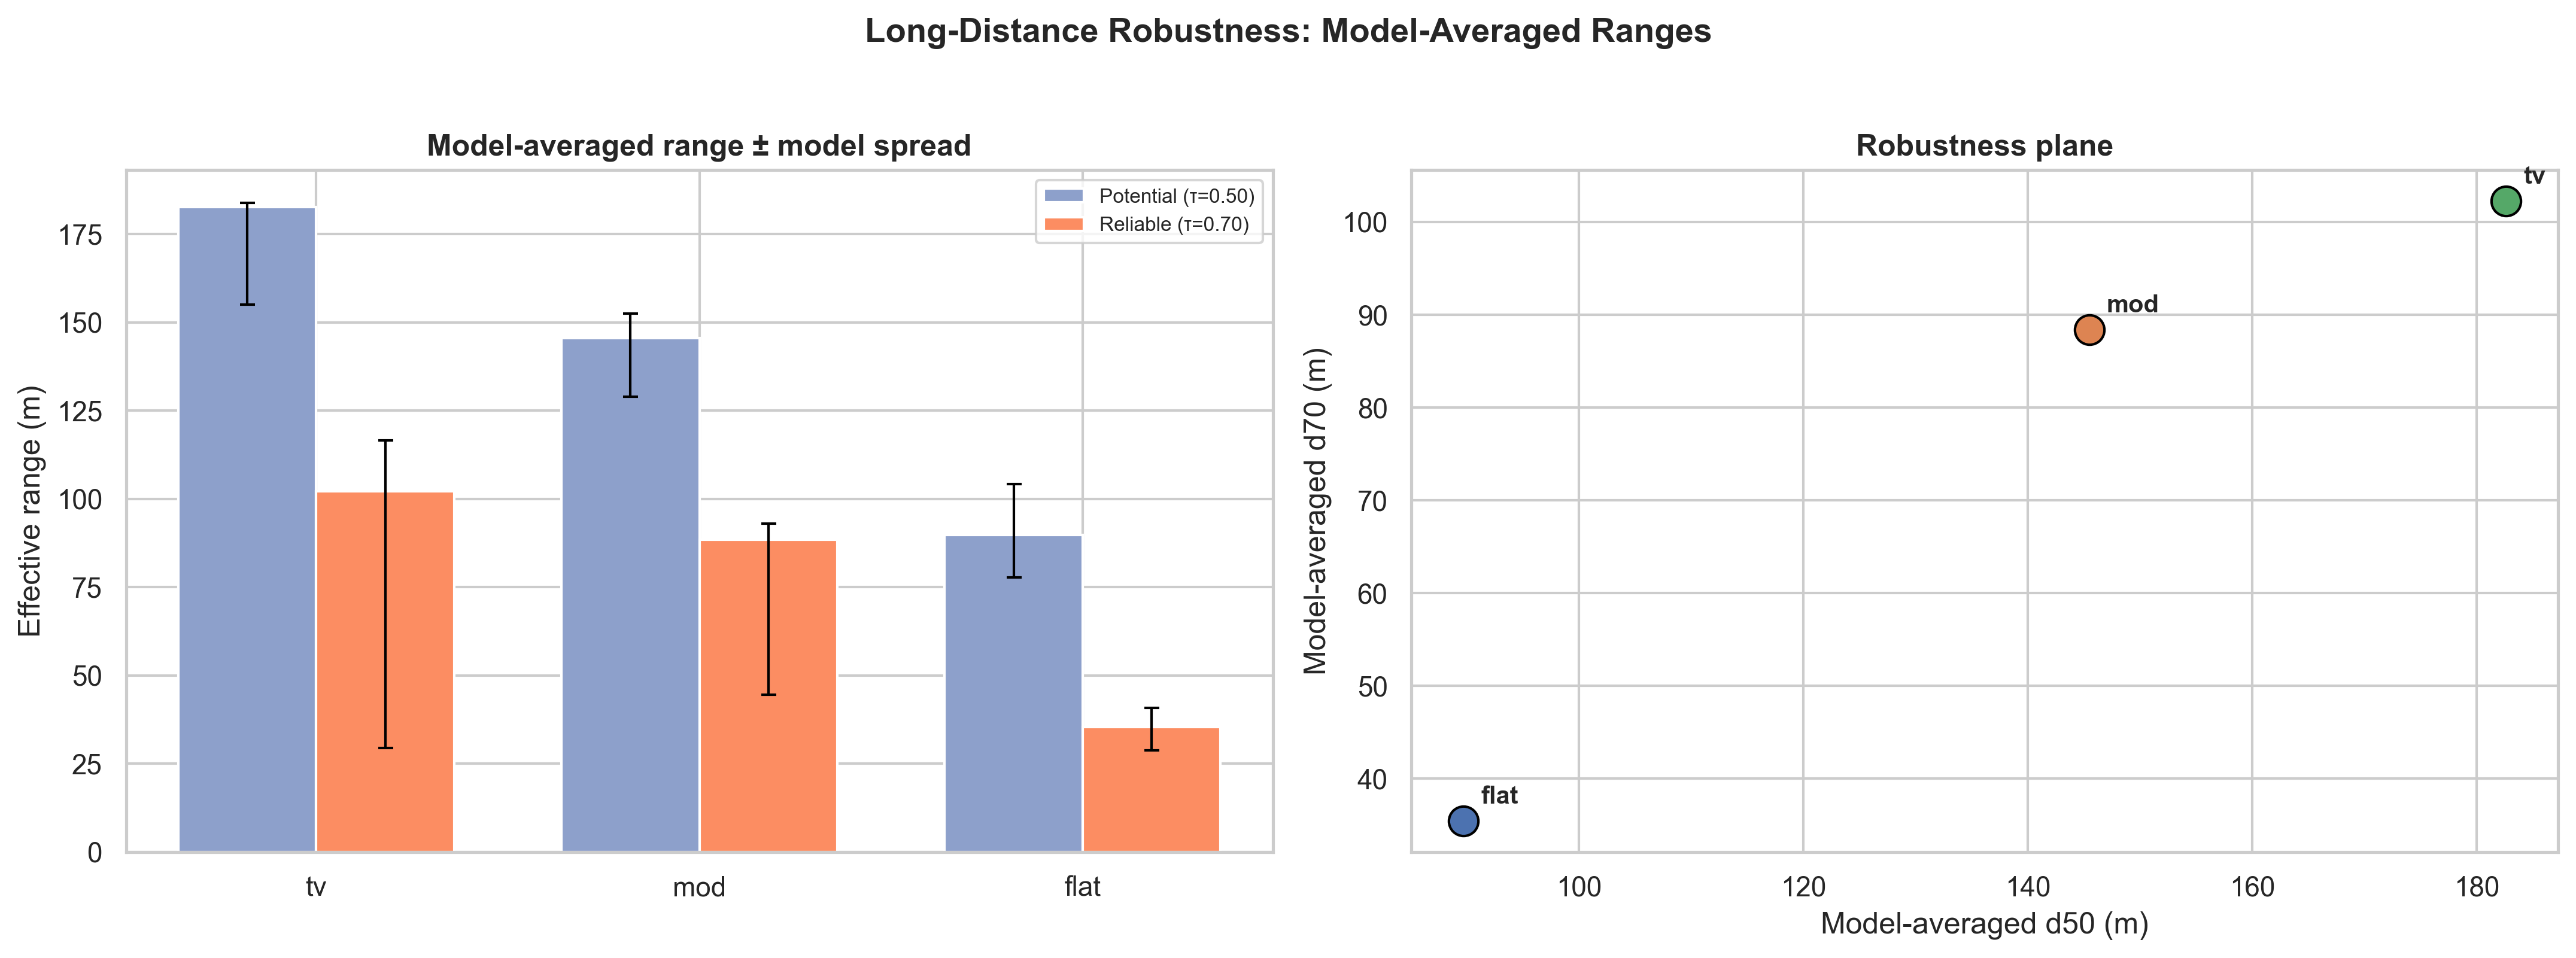
\includegraphics[width=\linewidth,height=.24\textheight,keepaspectratio]{../outputs_p2/P2_fig7_robustness_ranking.png}
    \caption{潜在识别与可靠识别标准下三类叫声的模型平均有效距离}\label{fig:p2_robustness}
\end{figure}
\clearpage

\section{问题三：海上回放实验行为响应与响应潜伏期建模}

\subsection{总体响应率对比与广义估计方程（GEE）协变量分析}

基于 \texttt{Data 02} 的 $139$ 对配对海上回放实验，同一场实验（expID）既放了自然叫声又放了对照，属于配对数据，不能用普通卡方检验。
本文采用\textbf{精确双侧 McNemar 检验}评估配对回放的总体响应差异，并构建按实验编号（\texttt{expID}）聚类的\textbf{二项 Logistic 广义估计方程}
量化叫声类型、行为情境、回放距离与群体规模的独立效应：
\begin{equation}\label{eq:p3_gee}
    \begin{aligned}
        \operatorname{logit}\,P(Y_{ij}=1)
        &= \beta_0 + \boldsymbol{\beta}_1^{\top}\text{CallType}_{ij}
          + \boldsymbol{\beta}_2^{\top}\text{Context}_{ij} \\
        &\quad + \beta_3\,\frac{\text{Distance}_{ij}-100}{50}
          + \beta_4\,\log_2\!\left(\frac{\text{Npenguins}_{ij}}{8}\right),
    \end{aligned}
\end{equation}

其中 $Y_{ij} \in \{0,1\}$ 表示第 $i$ 场实验第 $j$ 次回放是否诱发抬头（H）、发声（V）或接近（A）中任一行为。

结果显示，自然叫声与对照声音的总体响应率分别为 $64.7\%$（$90/139$）与 $12.9\%$（$18/139$），
相差 $51.8$ 个百分点。
同时McNemar 检验极显著（$p = 7.75 \times 10^{-20}$）。不同情境下，搜寻情境的自然叫声响应率最高（$36/38$，相对对照差值达 $81.6$ 个百分点），通勤（$35/65$）与摄食后（$19/36$）次之（见图~\ref{fig:p3_env} 上）。

表~\ref{tab:p3_gee} 与图~\ref{fig:p3_env} 下给出了共同斜率 GEE 估计结果：三类自然叫声均与极高的响应优势相关（\texttt{flat} $\text{OR} = 13.12$、\texttt{mod} $15.54$、\texttt{tv} $19.70$，均 $p < 0.001$）；
\textbf{群体规模翻倍时，记录到群体响应的优势显著下降约 $30\%$（$\text{OR} = 0.70, p = 0.010$）}；回放距离每增加 $50\text{ m}$ 的优势比为 $0.85$（$p = 0.424$）。

\begin{table}[htbp]
\centering
\caption{总体行为响应的共同斜率 GEE 估计结果（按 \texttt{expID} 聚类，稳健夹心标准误）}
\label{tab:p3_gee}
\footnotesize\setlength{\tabcolsep}{4pt}
\begin{tabular*}{.92\linewidth}{@{\extracolsep{\fill}}lccc@{}}
\toprule
变量 / 对比 & 调整后 OR & $95\%$ CI & $p$ 值 \\
\midrule
\texttt{flat} / 对照 & $13.12$ & $[6.15, 27.98]$ & $<0.001$ \\
\texttt{mod} / 对照 & $15.54$ & $[6.15, 39.23]$ & $<0.001$ \\
\texttt{tv} / 对照 & $19.70$ & $[8.58, 45.22]$ & $<0.001$ \\
\midrule
搜寻 / 通勤 & $1.76$ & $[0.72, 4.34]$ & $0.216$ \\
摄食后 / 通勤 & $1.04$ & $[0.44, 2.47]$ & $0.935$ \\
距离增加 $50\text{ m}$ & $0.85$ & $[0.58, 1.26]$ & $0.424$ \\
群体规模翻倍 & $0.70$ & $[0.54, 0.92]$ & $0.010$ \\
\bottomrule
\end{tabular*}
\end{table}

\begin{figure}[htbp]
    \centering
    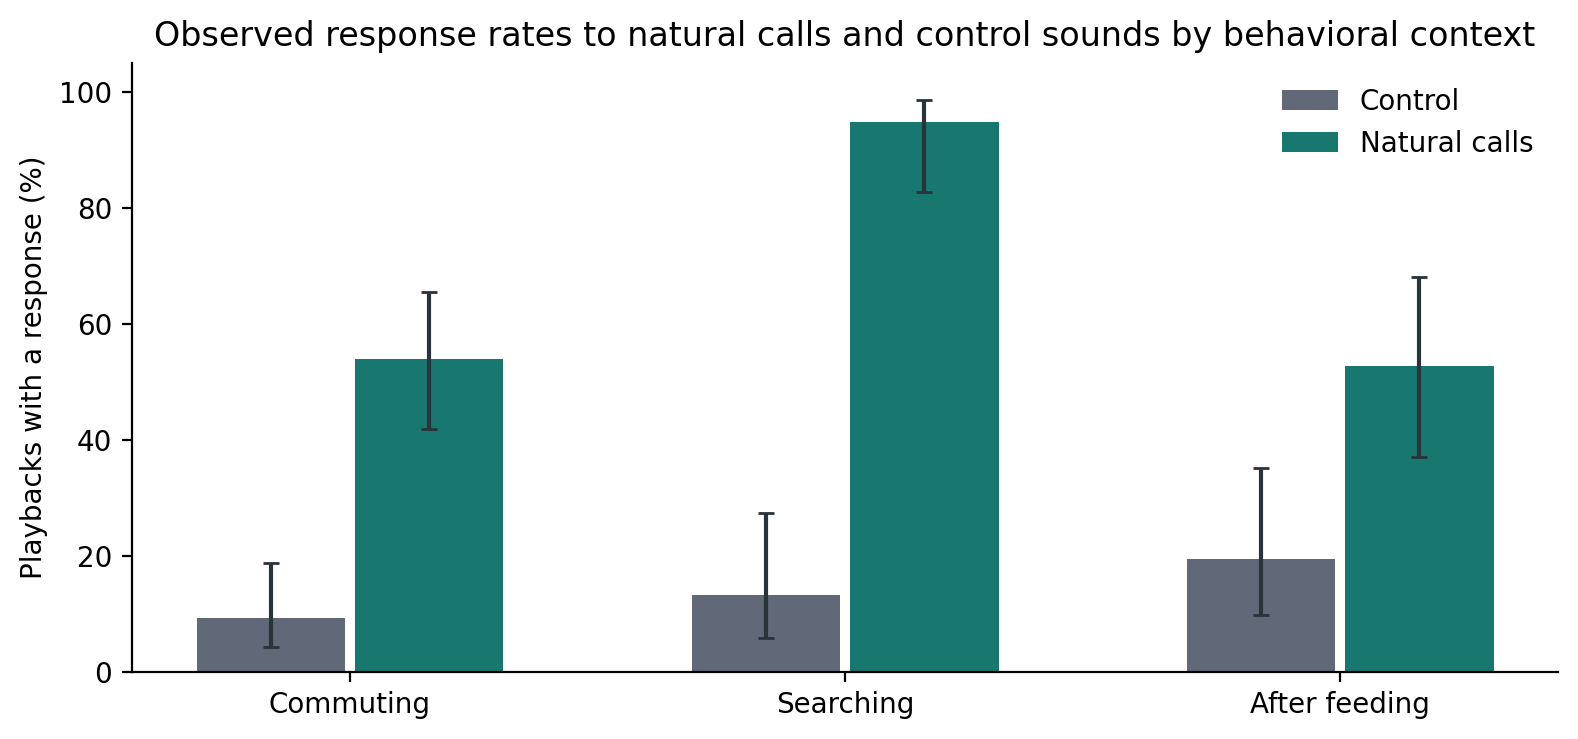
\includegraphics[width=.60\linewidth,height=.22\textheight,keepaspectratio]{../outputs_p3_part1/figures/02_context.png}\par\smallskip
    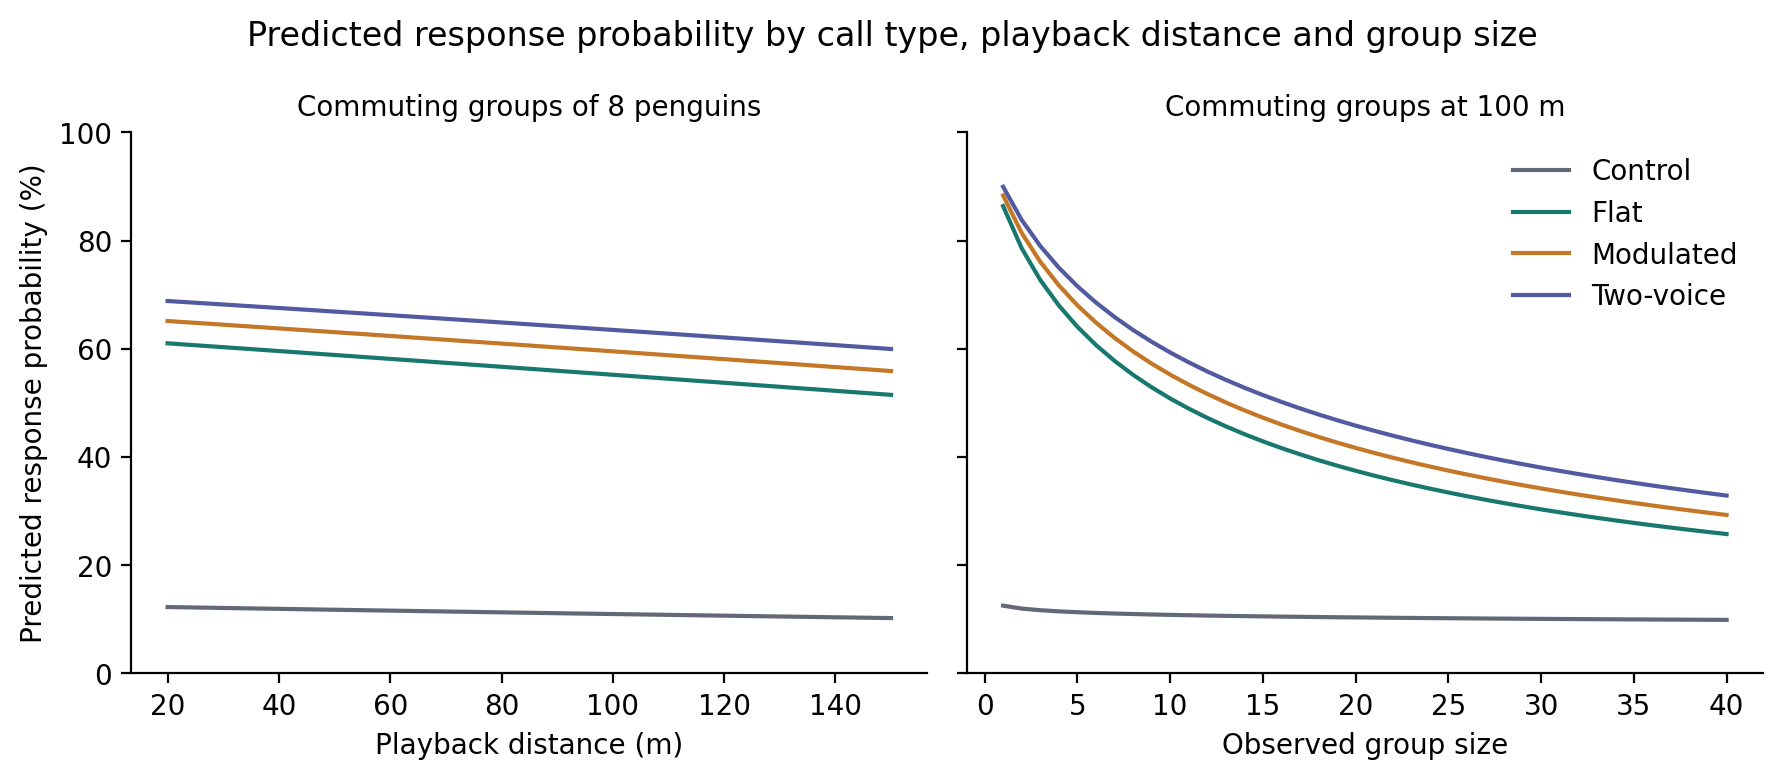
\includegraphics[width=.65\linewidth,height=.23\textheight,keepaspectratio]{../outputs_p3_part1/figures/03_environment.png}
    \caption{不同行为情境下自然叫声与对照响应率（上）及 GEE 预测响应概率随距离与群体规模变化（下）}
    \label{fig:p3_env}
\end{figure}

\subsection{八种行为组合的两阶段共现跨栏模型（Hurdle Pairwise）}

将抬头（H）、发声（V）与接近（A）的二元出现情况组合为 $2^3 = 8$ 种互斥状态（\texttt{None}, \texttt{H}, \texttt{V}, \texttt{A}, \texttt{HV}, \texttt{HA}, \texttt{VA}, \texttt{HVA}）。

为严格检验自然叫声是否改变了原始行为组合分布，记第 $i$ 场配对实验中自然叫声与对照的状态独热向量之差为 $\boldsymbol{\delta}_i = \mathbf{e}_{i,\text{call}} - \mathbf{e}_{i,\text{ctrl}} \in \{-1,0,1\}^8$，
构造八类边际计数差的平方和统计量，并在配对内标签可交换的原假设下通过随机翻号 $\xi_i^{(b)} \in \{-1, +1\}$ 执行 $B = 10^5$ 次配对置换检验：
\begin{equation}\label{eq:p3_perm}
    T_{\text{obs}} = \left\|\sum_{i=1}^{139} \boldsymbol{\delta}_i\right\|_2^2, \qquad
    T^{(b)} = \left\|\sum_{i=1}^{139} \xi_i^{(b)}\boldsymbol{\delta}_i\right\|_2^2, \qquad
    p = \frac{1 + \sum_{b=1}^{B} \mathbb{I}\bigl(T^{(b)} \ge T_{\text{obs}}\bigr)}{B + 1}.
\end{equation}

结果显示 $10^5$ 次置换均未达到观测值（$p = 1/100001 \approx 10^{-5}$），证实自然叫声极显著地改变了行为组合分布。由于部分配对实验的回放距离不同，下文进一步\textbf{建立条件概率模型}在统一协变量框架下比较各叫声类型。

为克服稀有组合（如 \texttt{A}, \texttt{HA}, \texttt{VA}）样本稀疏问题并在统一框架下比较三类叫声，本文构建\textbf{两阶段共现跨栏模型（Hurdle Pairwise Model）}，并与传统岭惩罚八分类多项回归（Multinomial）及无共现项的加性跨栏模型（Hurdle Additive）对比：
\begin{equation}\label{eq:p3_hurdle}
    \begin{aligned}
        P(\text{None}\mid\mathbf{x}) &= 1-r(\mathbf{x}), \\
        P(s\mid\mathbf{x}) &= r(\mathbf{x})\,
        \frac{\exp\bigl(u(s,\mathbf{x})\bigr)}
             {\sum_{s'\neq\text{None}}\exp\bigl(u(s',\mathbf{x})\bigr)}
        \qquad(s\neq\text{None}),
    \end{aligned}
\end{equation}

\begin{equation}\label{eq:p3_utility}
    u(s, \mathbf{x}) = h\,\eta_h(\mathbf{x}) + v\,\eta_v(\mathbf{x}) + a\,\eta_a(\mathbf{x}) + \kappa_1 hv + \kappa_2 ha + \kappa_3 va,
\end{equation}
其中发生层 $r(\mathbf{x}) = \operatorname{expit}(\mathbf{x}^\top \mathbf{w})$ 估计任意响应概率；构成层中 $(h,v,a) \in \{0,1\}^3 \setminus \{(0,0,0)\}$ 为行为指示位，线性预测子 $\eta_h, \eta_v, \eta_a$ 在所有包含对应行为的组合间\textbf{共享参数}（大幅提升稀疏状态估计精度），成对共现项 $\kappa_1, \kappa_2, \kappa_3$ 刻画行为协同偏离，并施加 $L_2$ 岭惩罚防止过拟合。

\textbf{模型验证与标准化对比}：
在 $10 \times 5$ 折实验留出与 $12$ 日逐日留出交叉验证中，Hurdle Pairwise 的八态对数损失均最低（实验留出 $1.1151$，显著优于传统多项回归 $1.1615$，$p = 1.32 \times 10^{-11}$，
亦优于加性跨栏模型 $1.1211$ 与边际基线 $1.287$；日期留出 $1.1145$ vs. $1.1478$），
且在惩罚强度 $0.25\times$--$4\times$ 及 $20\text{--}150\text{ m}$ 共同距离下均保持稳健，
表明该模型可行且预测更优。图~\ref{fig:p3_states} 展示了按 $278$ 条记录的协变量分布标准化后的八种行为组合概率。表~\ref{tab:p3_contrasts} 给出了组间概率差及基于 $1500$ 次整对 Bootstrap 的同时置信区间。
自然叫声相对对照总体响应率提高 $+50.7$ 个百分点（同时 $95\%$ CI $[35.0, 66.3]$），
增量主要集中在\textbf{仅发声（V，$+17.8$ pp）}、\textbf{抬头伴发声（HV，$+17.9$ pp）}与\textbf{三者齐现（HVA，$+8.0$ pp）}；
而三类自然叫声两两直接对比的同时区间均包含零，尚不足以断言某类叫声在特定组合上绝对占优。

\begin{table}[htbp]
\centering
\caption{标准化后主要行为组合的概率差及同时 $95\%$ 置信区间（单位：百分点）}
\label{tab:p3_contrasts}
\footnotesize\setlength{\tabcolsep}{4pt}
\begin{tabular*}{.92\linewidth}{@{\extracolsep{\fill}}llc@{}}
\toprule
对比组 & 行为组合 & 概率差 $[\text{同时 }95\%\text{ CI}]$ \\
\midrule
自然叫声 / 对照 & 仅发声（V） & $+17.8\,[+5.9, +29.7]$ \\
自然叫声 / 对照 & 抬头+发声（HV） & $+17.9\,[+7.1, +28.6]$ \\
自然叫声 / 对照 & 三者齐现（HVA） & $+8.0\,[+0.2, +15.8]$ \\
\midrule
\texttt{flat} / 对照 & 抬头+发声（HV） & $+24.1\,[+5.8, +42.4]$ \\
\texttt{mod} / 对照 & 抬头+发声（HV） & $+16.2\,[+0.03, +32.3]$ \\
\texttt{tv} / 对照 & 仅发声（V） & $+23.4\,[+4.6, +42.3]$ \\
\texttt{tv} / 对照 & 抬头+发声（HV） & $+13.7\,[+1.9, +25.5]$ \\
\bottomrule
\end{tabular*}
\par\smallskip{\scriptsize\raggedright 注：三种自然叫声两两比较的同时置信区间均包含零。\par}
\end{table}

\begin{figure}[htbp]
    \centering
    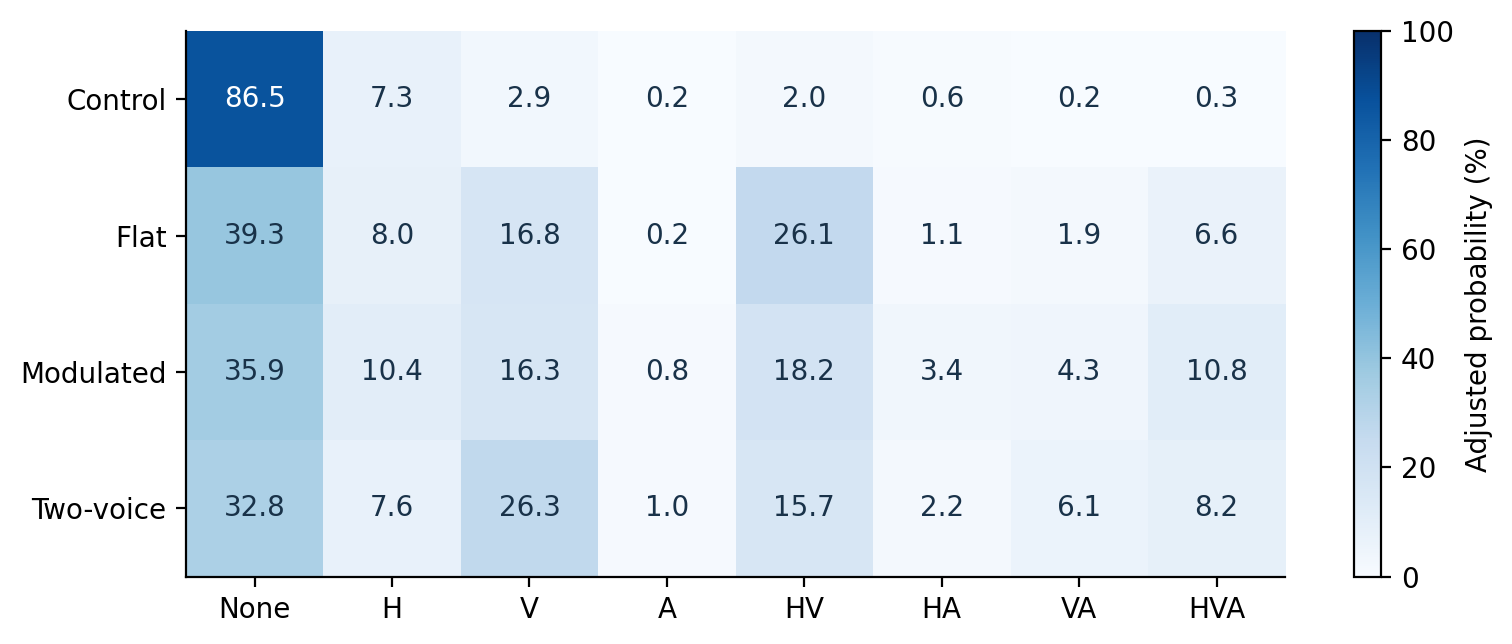
\includegraphics[width=.75\linewidth,height=.22\textheight,keepaspectratio]{../outputs_p3_part1/figures/05_adjusted_states.png}
    \caption{四种回放条件下八种行为组合的标准化概率热图}
    \label{fig:p3_states}
\end{figure}

\subsection{响应潜伏期（零膨胀 AFT）与条件响应强度建模}

针对三项具体行为及``首次任意响应''共 $4$ 个时间终点，本文建立\textbf{含零点质量的对数正态加速失效时间模型（Zero-inflated Log-normal AFT）}以刻画观测中存在的 $0\text{ s}$ 即时抬头与即时首次响应；对正潜伏期样本（$T_{ik} > 0$）施加岭正则化，并在 $5 \times 5$ 折实验留出 CV 下比较 Separate AFT、\textbf{Separate Ridge AFT（主模型，交叉验证选优惩罚 $\lambda = 256$）}与部分共享斜率 Shared AFT：
\begin{equation}\label{eq:p3_aft}
    \begin{aligned}
        \ln T_{ik}\mid(T_{ik}>0,\mathbf{x}_i)
        &\sim \mathcal{N}\bigl(\mathbf{x}_i^\top\boldsymbol{\beta}_k,\sigma_k^2\bigr),\\
        Q_\alpha(T_k\mid\mathbf{x})
        &= \begin{cases}
              0, & 0<\alpha\leq\pi_{0k},\\[2pt]
              \exp\!\left(\mathbf{x}^\top\boldsymbol{\beta}_k+\sigma_k\,
              \Phi^{-1}\!\left(\dfrac{\alpha-\pi_{0k}}{1-\pi_{0k}}\right)\right),
                & \pi_{0k}<\alpha<1 .
           \end{cases}
    \end{aligned}
\end{equation}
其中 $\pi_{0k}$ 为第 $k$ 个终点的即时零点概率估计。在留出验证中（见图~\ref{fig:p3_timing}），主模型 Separate Ridge AFT 在抬头（MAE $= 1.40\text{ s}$，$90\%$ 覆盖率 $90.6\%$）、发声（$2.98\text{ s}$，覆盖率 $92.1\%$）与首次任意响应（$2.23\text{ s}$，覆盖率 $93.7\%$）上误差均低于无正则化 AFT，且在稀疏接近行为上（$23$ 次事件，MAE $= 5.53\text{ s}$）显著抑制了方差膨胀。

对响应者的条件强度，采用两类岭回归模型：（1）对发声次数（\texttt{VocalNcalls} $\ge 1$）建立控制回放前基线发声 $\ln(1 + \text{VocalNcallsBefore})$ 的\textbf{移位泊松岭回归} $\mathbb{E}[Y_{\text{voc}} - 1 \mid \mathbf{x}] = \exp(\mathbf{x}^\top\boldsymbol{\gamma}_v)$；（2）对抬头时长与接近时长建立\textbf{带 Duan 涂抹校正（Smearing）的对数线性岭回归} $\mathbb{E}[Y_k \mid \mathbf{x}] = \hat{\phi}_k \exp(\mathbf{x}^\top\boldsymbol{\gamma}_k)$。交叉验证表明，非耦合强度模型在接近时长（MAE $16.90\text{ s}$ vs. $17.00\text{ s}$）与发声次数（$2.249$ vs. $2.254$）上略优于潜伏期耦合模型，故主模型采用非耦合设定。

\begin{figure}[htbp]
    \centering
    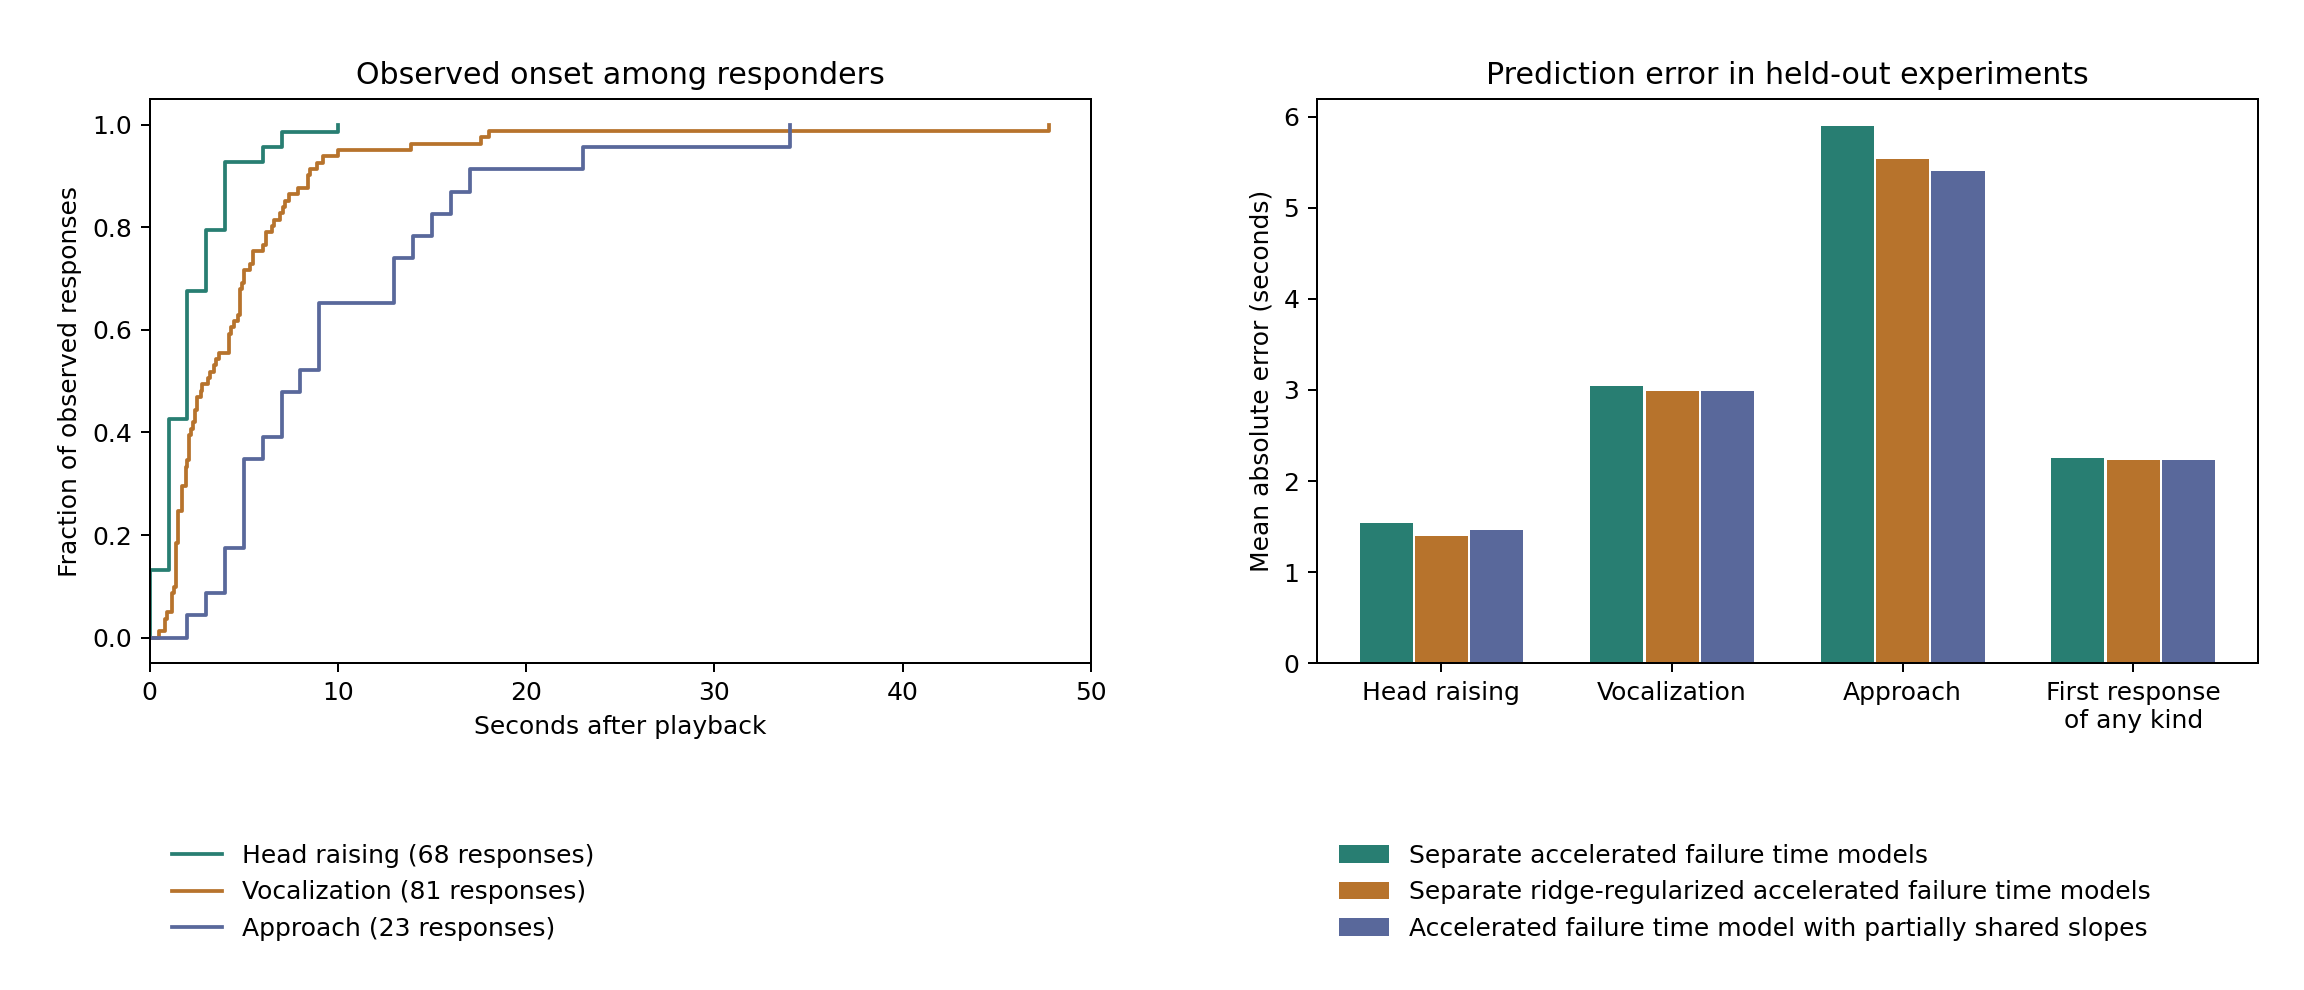
\includegraphics[width=\linewidth,height=.25\textheight,keepaspectratio]{../outputs_p3_part2/figures/04_timing_validation.png}
    \caption{响应者各行为启动时间经验累积分布（左）及三类 AFT 模型在留出实验中的 MAE 对比（右）}
    \label{fig:p3_timing}
\end{figure}

\subsection{代表性条件数值预测表与稳健性边界}

严格按题目要求，将群体规模设为观测中位数（$\text{Npenguins} = 8$），对行为情境按经验分布加权标准化（通勤 $46.8\%$、搜寻 $27.3\%$、摄食后 $25.9\%$），通过混合 CDF 二分法求解 $50\text{ m}, 100\text{ m}, 150\text{ m}$ 处的中位响应潜伏期，并结合 $500$ 次整对 Bootstrap 给出 $95\%$ 置信区间（见表~\ref{tab:p3_pred}）；凡在该刺激类型与距离下未观测到对应响应的单元，均严格记为``无响应''。

\begin{table}[htbp]
\centering
\caption{代表性条件下（$\text{Npenguins}=8$，情境标准化）各叫声类型中位响应潜伏期预测表（单位：$\text{s}$，$[95\%\text{ CI}]$）}
\label{tab:p3_pred}
\footnotesize\setlength{\tabcolsep}{2.5pt}
\begin{tabular*}{\linewidth}{@{\extracolsep{\fill}}lcccccc@{}}
\toprule
回放声音 & 距离 ($\text{m}$) & 试次数 & 抬头潜伏期 & 发声潜伏期 & 接近潜伏期 & 首次任意响应 \\
\midrule
Control & $50$ & $19$ & 无响应 & $3.2\,[2.7, 3.9]$ & 无响应 & $1.8\,[1.3, 2.8]$ \\
Control & $100$ & $22$ & $1.8\,[1.5, 2.2]$ & $3.4\,[2.8, 4.0]$ & 无响应 & $2.0\,[1.4, 3.2]$ \\
Control & $150$ & $8$ & $1.8\,[1.5, 2.2]$ & 无响应 & 无响应 & $2.3\,[1.5, 4.0]$ \\
\midrule
\texttt{flat} & $50$ & $4$ & $1.8\,[1.5, 2.2]$ & $3.2\,[2.6, 3.8]$ & $8.0\,[6.1, 10.3]$ & $1.9\,[1.4, 2.5]$ \\
\texttt{flat} & $100$ & $14$ & $1.8\,[1.5, 2.2]$ & $3.3\,[2.8, 3.9]$ & 无响应 & $2.1\,[1.5, 2.8]$ \\
\texttt{flat} & $150$ & $3$ & 无响应 & $3.4\,[2.9, 4.1]$ & 无响应 & $2.4\,[1.6, 3.6]$ \\
\midrule
\texttt{mod} & $50$ & $8$ & $1.8\,[1.5, 2.2]$ & $3.2\,[2.6, 3.7]$ & $8.0\,[6.1, 10.3]$ & $1.7\,[1.3, 2.3]$ \\
\texttt{mod} & $100$ & $5$ & 无响应 & 无响应 & 无响应 & 无响应 \\
\texttt{mod} & $150$ & $3$ & 无响应 & $3.4\,[2.9, 4.1]$ & $8.4\,[6.2, 11.1]$ & $2.2\,[1.5, 3.5]$ \\
\midrule
\texttt{tv} & $50$ & $9$ & $1.8\,[1.5, 2.2]$ & $3.2\,[2.7, 3.9]$ & $8.0\,[6.1, 10.4]$ & $2.6\,[2.0, 3.3]$ \\
\texttt{tv} & $100$ & $11$ & $1.9\,[1.5, 2.2]$ & $3.4\,[2.8, 4.0]$ & $8.2\,[6.1, 10.8]$ & $2.9\,[2.3, 3.8]$ \\
\texttt{tv} & $150$ & $2$ & $1.9\,[1.5, 2.3]$ & $3.5\,[3.0, 4.2]$ & 无响应 & $3.3\,[2.4, 4.8]$ \\
\bottomrule
\end{tabular*}
\par\smallskip{\scriptsize\raggedright 注：试次数为该刺激和距离下所有群体规模的实测次数。潜伏期为响应者在标准化条件下的中位数。``无响应''表示该距离下存在回放试次但未记录到对应行为，并不意味着企鹅未感知到声学刺激；响应者平均强度在 $50\text{--}150\text{ m}$ 内保持稳定（抬头时长约 $17.5\text{--}25.5\text{ s}$，发声次数约 $2.5\text{--}4.5$ 次，接近时长约 $27.9\text{--}41.9\text{ s}$）。\par}
\end{table}

综合表~\ref{tab:p3_pred} 与距离对比检验可见：（1）\textbf{行为启动呈清晰的时序级联}：抬头最快（中位 $1.8\text{--}1.9\text{ s}$）、发声居中（$3.2\text{--}3.5\text{ s}$）、接近最慢（$8.0\text{--}8.4\text{ s}$），首次任意响应中位时间约 $1.7\text{--}3.3\text{ s}$；（2）\textbf{距离延长仅引起轻微延迟}：从 $50\text{ m}$ 增至 $150\text{ m}$，首次响应延迟约 $+0.51\text{--}+0.76\text{ s}$、发声延迟约 $+0.27\text{ s}$，但 $95\%$ 差值置信区间均包含零；（3）\textbf{审计敏感性稳健}：针对原始数据中极少数未标记响应却含正潜伏期/强度记录的条目（发声 $4$ 条、接近 $5$ 条），将其纳入响应重跑模型后中位潜伏期与强度预测均无实质偏移，验证了主结论的稳健性。
\clearpage

\section{问题四：海上声学通信有效性评估、噪声情景分析与保护建议}

为综合前序声学保真度、行为组合概率与环境情境形成可落地的生态保护决策，本节按``通信有效性指数构建与有效半径估计、单次回放期望响应个体数分析、噪声与恶劣海况压力测试、实验改进与栖息地保护建议''四个阶段依次展开。

\subsection{阶段一：海上声学通信有效性综合指数与有效通信半径}

本阶段融合第二问的单调递减保真度曲线 $F_t(d)$（PCA 融合权重 $0.338 / 0.340 / 0.322$）与第三问的八状态联合概率模型 $p(s \mid d, c, N)$，构建面向群体联络与聚集的\textbf{海上声学通信有效性综合指数}。首先，采用\textbf{层次分析法（AHP）}确立四项行为效用权重：构造体现``靠近（招募）$>$ 发声（联络）$>$ 抬头（警觉）''生态取向的 $4 \times 4$ 判断矩阵（相对重要性依次为 $1, 2, 8/3, 1$），求得最大特征值 $\lambda_{\max} = 4$、一致性比率 $\text{CR} = 0$，归一化主特征向量给出抬头 $0.15$、发声 $0.30$、靠近 $0.40$、出现至少两类行为共现加分 $0.15$。据此定义行为组合效用 $u(s)$、预期效用 $B_t$ 及百分制综合有效性指数 $I_t$：
\begin{equation}\label{eq:p4_index}
    \begin{aligned}
        u(s) &= 0.15\,h + 0.30\,v + 0.40\,a + 0.15\,\mathbb{I}(h + v + a \ge 2), \\
        B_t(d, c, N) &= \sum_{s} p_t(s \mid d, c, N)\,u(s),
    \end{aligned}
\end{equation}
\begin{equation}\label{eq:p4_score}
    I_t(d, c, N) = 100 \cdot F_t(d) \cdot \max\bigl(0,\; B_t(d, c, N) - B_0(d, c, N)\bigr),
\end{equation}
其中 $B_0$ 为同条件下对照声音的预期效用，扣除背景后截取正部以仅评价高于背景的行为净增益；乘积结构保证低保真度或低行为增益均会压低得分。模型核验显示，上游 P2 半径与 P3 概率的复现误差均 $< 10^{-10}$；对可观测行为效用执行 $5 \times 5$ 折实验留出验证，八状态模型 RMSE 为 $0.235$，优于仅按叫声类型取均值的基线（$0.249$）。

将群体规模固定为中位数 $N = 8$ 只，按经验情境比例（通勤 $130/278$、搜寻 $76/278$、摄食后 $72/278$）加权标准化。预设主有效阈值为 $15$ 分（对应保真度 $0.60$、行为净增益 $0.25$ 的参照组合，约合三类叫声近源指数 $25.5 / 28.9 / 25.2$ 分的 $52\%\text{--}60\%$），并通过 $1000$ 次双来源重采样（声学按试次轨迹整条重抽、回放按 $139$ 对 \texttt{expID} 整对重抽）估计 $95\%$ 置信区间，同时检验 $5$ 套替代权重与 $8\text{--}24$ 分阈值敏感性（见表~\ref{tab:p4_radii} 与图~\ref{fig:p4_index}）。结果显示，情境标准化有效半径依次为 \texttt{flat} $74.9\text{ m}$、\texttt{mod} $125.4\text{ m}$、\texttt{tv} $144.3\text{ m}$，搜寻情境下三类半径均达最大（\texttt{tv} 达 $171.9\text{ m}$）。但在 $100\text{ m}$ 处，\texttt{tv}（$19.3$ 分）与 \texttt{mod}（$18.4$ 分）仅相差 $0.92$ 分（$95\%$ CI $[-6.45, 9.10]$），且当标准提高至 $22$ 分时 \texttt{mod} 点估计反超 \texttt{tv}，说明二者远距离排序仍具较大抽样与标准依赖性。

\begin{table}[htbp]
\centering
\caption{典型 $8$ 只群体在 $15$ 分主标准下的有效通信半径（单位：$\text{m}$）及权重敏感性对比}
\label{tab:p4_radii}
\footnotesize\setlength{\tabcolsep}{3.5pt}
\begin{tabular*}{\linewidth}{@{\extracolsep{\fill}}lccc|ccc|ccc@{}}
\toprule
叫声 & 通勤 & 搜寻 & 摄食后 & \shortstack{情境\\标准化} & \shortstack{观测内\\$95\%$ CI} & \shortstack{触上界\\比例} & \shortstack{行为\\等权} & \shortstack{侧重\\发声} & \shortstack{侧重\\靠近} \\
\midrule
\texttt{flat} & $69.8$ & $100.3$ & $50.2$ & $74.9$ & $[25.6, 102.1]$ & $0.0\%$ & $82.9$ & $99.0$ & $52.4$ \\
\texttt{mod} & $120.1$ & $\ge 150$ & $100.2$ & $125.4$ & $[76.8, 150.0]$ & $16.0\%$ & $132.1$ & $\ge 150$ & $107.3$ \\
\texttt{tv} & $140.1$ & $171.9$ & $113.0$ & $144.3$ & $[78.1, 192.7]$ & $1.3\%$ & $148.3$ & $182.6$ & $114.2$ \\
\bottomrule
\end{tabular*}
\par\smallskip{\scriptsize\raggedright 注：``$\ge 150$''表示至该组观测上界时指数仍高于 $15$ 分；若取严格三情境共同覆盖上界，\texttt{mod} 仅报告 $\ge 120\text{ m}$。\par}
\end{table}

\begin{figure}[htbp]
    \centering
    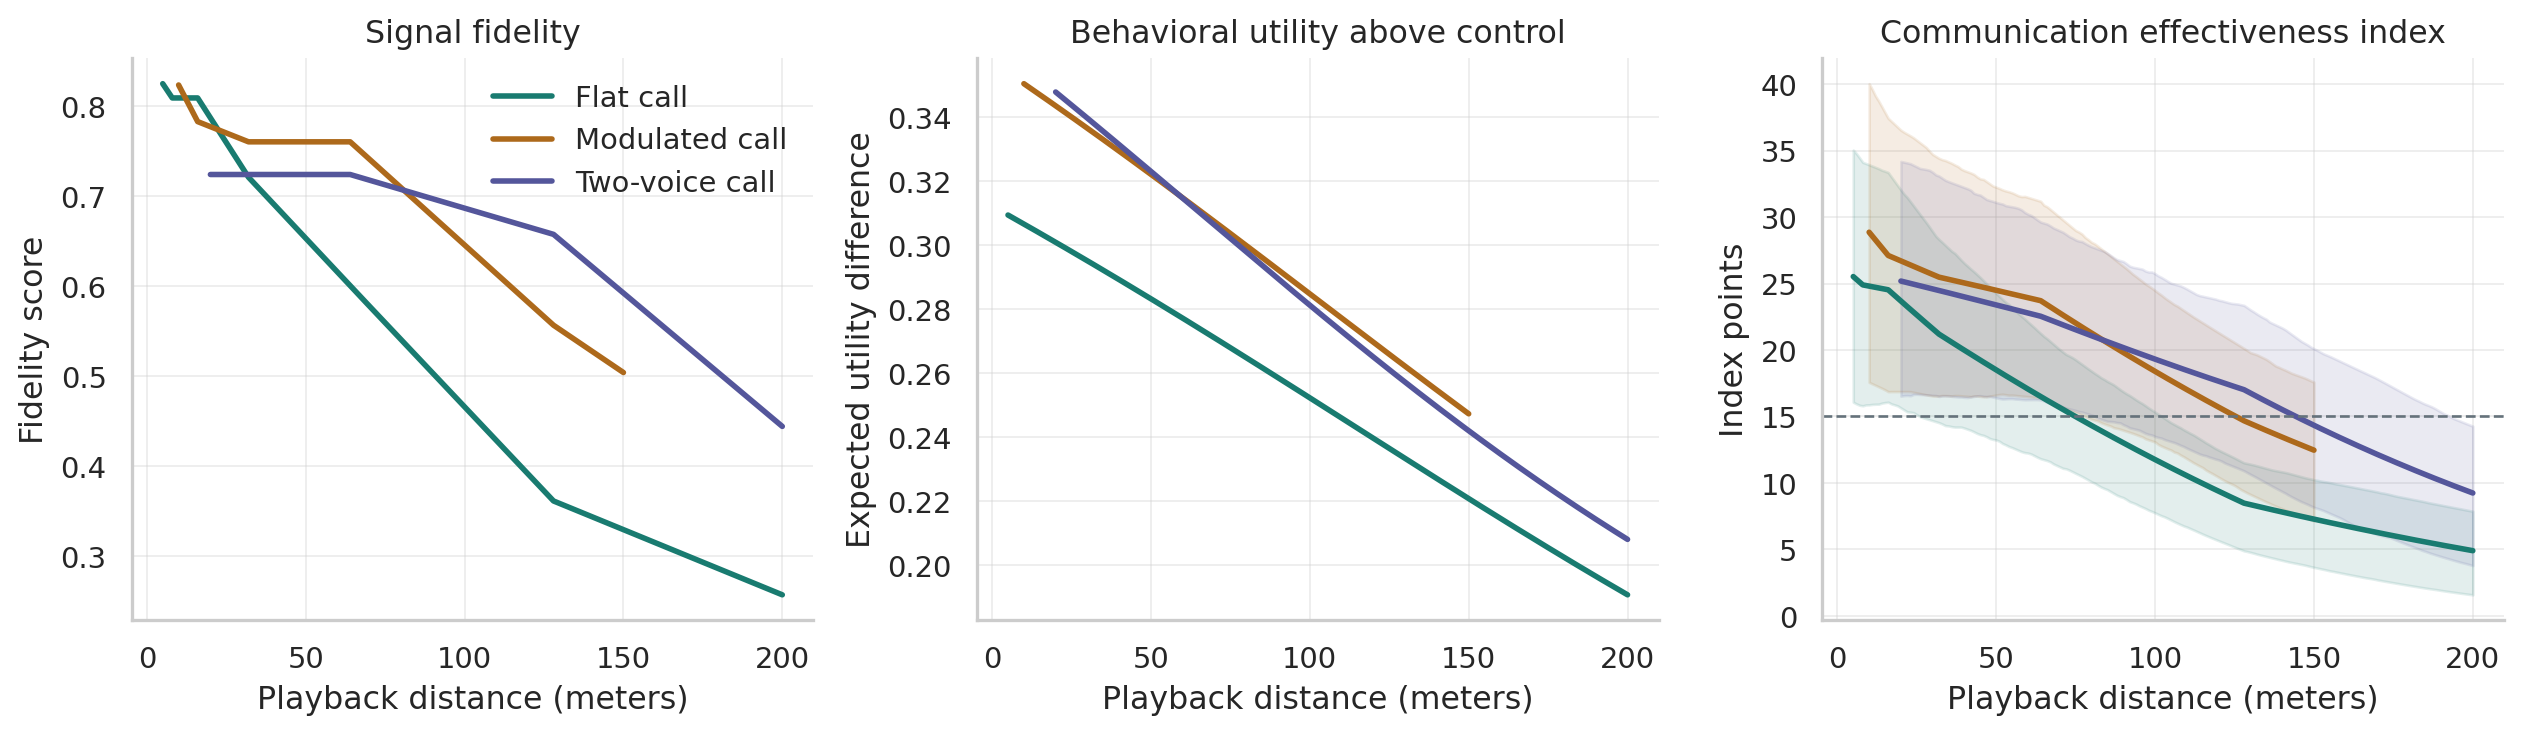
\includegraphics[width=\linewidth,height=.22\textheight,keepaspectratio]{../outputs_p4_part1/figures/01_index_components.png}\par\smallskip
    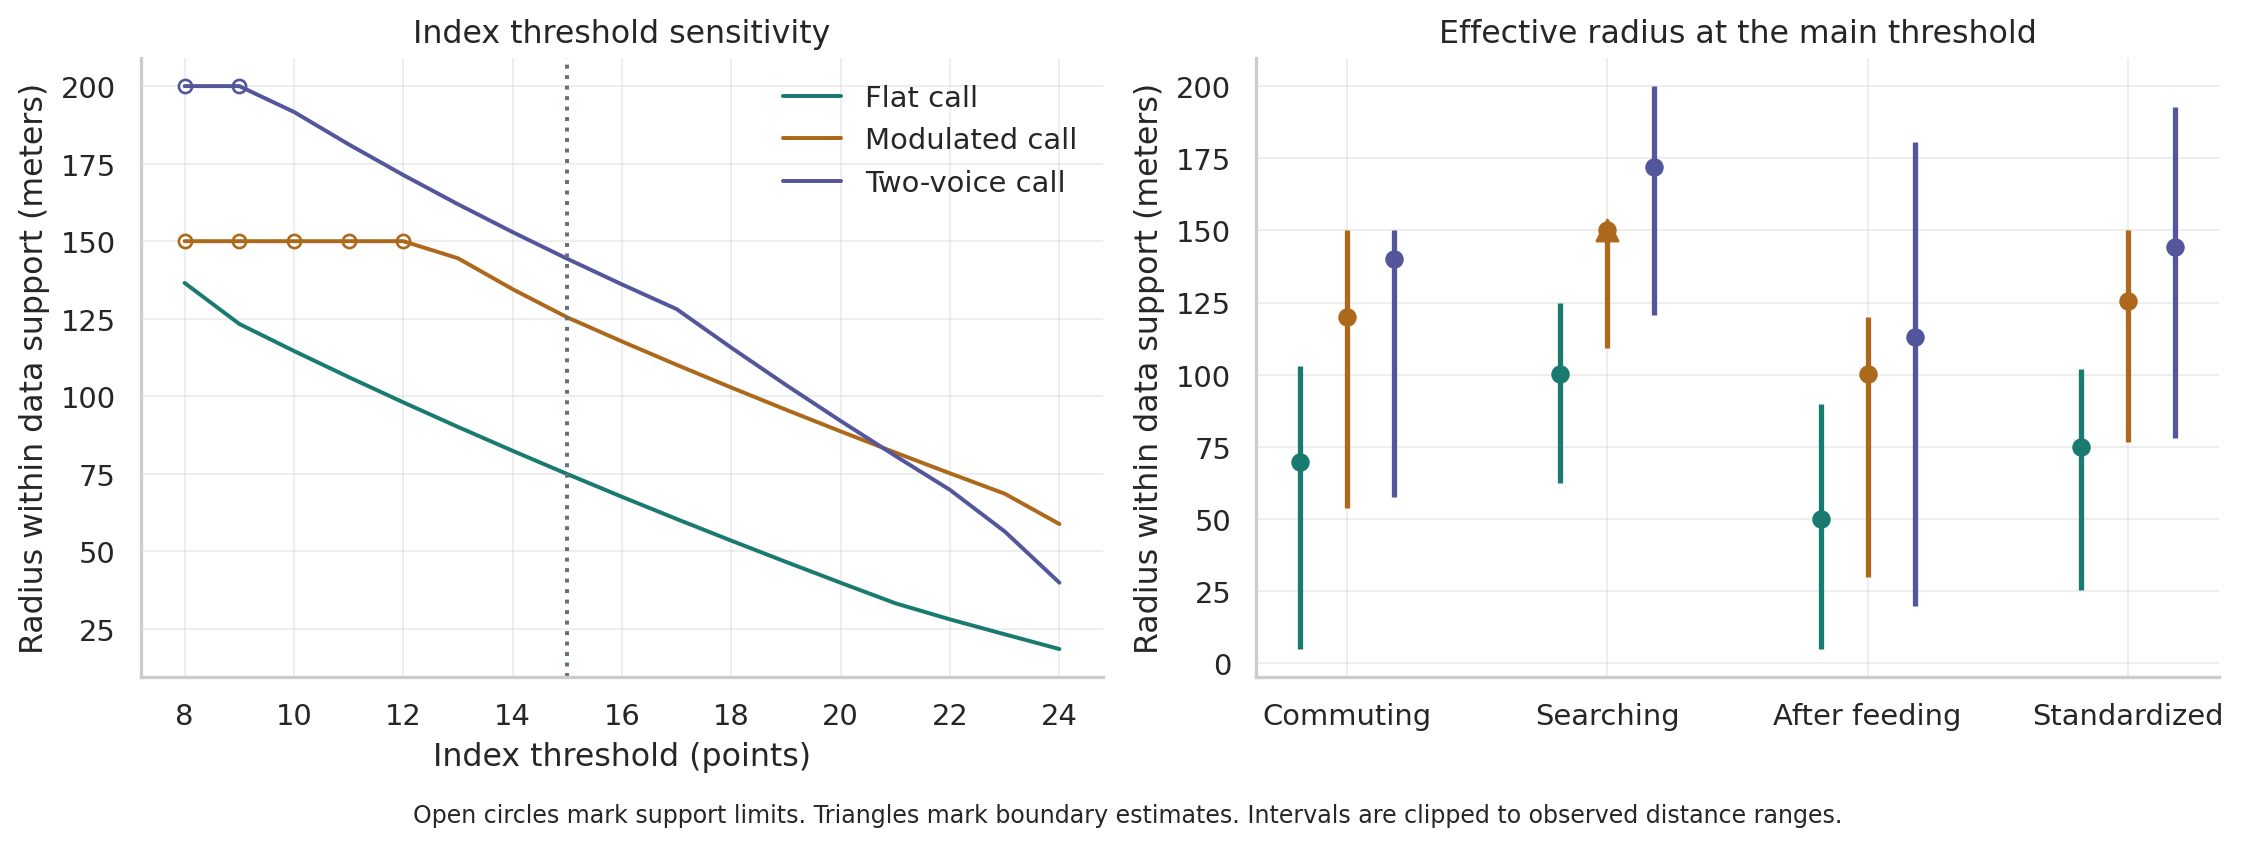
\includegraphics[width=\linewidth,height=.23\textheight,keepaspectratio]{../outputs_p4_part1/figures/03_effective_radius.png}
    \caption{信号保真度、行为净增益与综合有效性指数曲线（上）及阈值敏感性与各情境有效半径（下）}
    \label{fig:p4_index}
\end{figure}

\subsection{阶段二：单次回放期望响应个体数与群体规模敏感性}

由于原始回放数据仅记录群体层面的响应有无而未逐只计数，令 $K$ 为单次回放诱发的响应个体数，$\rho \in [1/N, 1]$ 为已响应群体内平均参与比例，由全期望公式得期望响应个体数；同时借用第三问 GEE 的群体规模斜率（$\beta = \ln 0.705$）外推不同群体规模 $N \in \{2, 4, 8, 16, 32\}$ 下的响应变化：
\begin{equation}\label{eq:p4_birds}
    \begin{aligned}
        \mathbb{E}(K) &= P(K \ge 1)\,\mathbb{E}(K \mid K \ge 1) = (1 - p_{000})\,N\rho, \\
        P(N) &= \operatorname{clip}\!\left(P(8)\left(\frac{N}{8}\right)^{\beta},\,0,\,1\right).
    \end{aligned}
\end{equation}

如图~\ref{fig:p4_part} 所示，在典型 $8$ 只群体、$100\text{ m}$ 距离下，若已响应群体平均有一半成员参与（$\rho = 50\%$），\texttt{flat}、\texttt{mod}、\texttt{tv} 每次回放期望引起响应的个体数依次为 $2.39$、$2.55$ 与 $2.69$ 只；当 $\rho$ 由 $25\%$ 增至 $75\%$ 时，三类期望响应数等比例增至 $3$ 倍（$1.19 / 1.27 / 1.35$ 只升至 $3.58 / 3.82 / 4.04$ 只）。进一步沿群体规模外推发现，尽管单只企鹅的人均响应率随群体增大而下降（如 $\rho=0.5$ 时，\texttt{flat} 在 $50\text{ m}$ 处由 $N=8$ 时的 $0.316$ 降至 $N=32$ 时的 $0.194$），但全群总期望响应个体数仍随 $N$ 单调上升。

\begin{figure}[htbp]
    \centering
    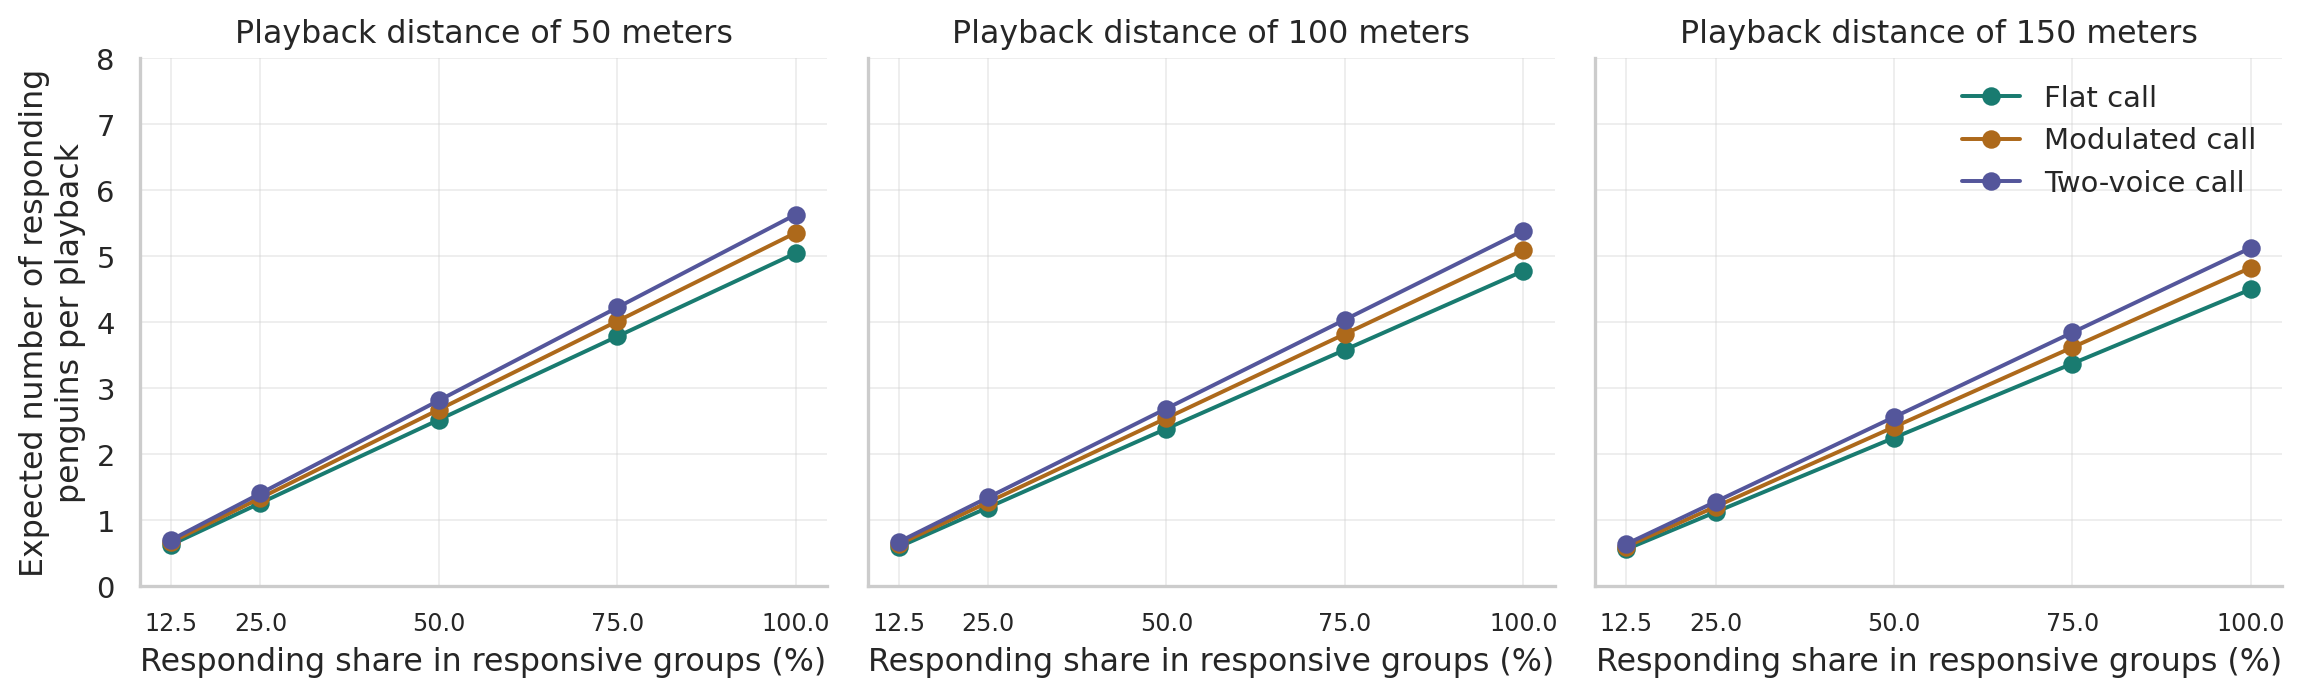
\includegraphics[width=\linewidth,height=.22\textheight,keepaspectratio]{../outputs_p4_part1/figures/04_participation_sensitivity.png}
    \caption{典型 $8$ 只群体在 $50, 100, 150\text{ m}$ 处期望响应个体数随群体内参与比例 $\rho$ 的敏感性变化}
    \label{fig:p4_part}
\end{figure}

\subsection{阶段三：环境噪声与恶劣海况的 $3 \times 5$ 全因子压力测试}

为量化背景噪声增强或恶劣海况对通信半径与响应概率的削弱，我们构造 $3 \times 5 = 15$ 个全因子压力情景：识别相关性阈值 $\tau \in \{0.50, 0.60, 0.70\}$，各距离相对保真度损失 $\delta \in \{0\%, 5\%, 10\%, 15\%, 20\%\}$。模型区分两条物理--行为传导通道：（1）物理保真度直接折减为 $(1 - \delta)F_t(d)$；（2）基于共同完整声学轨迹（\texttt{flat} $230$、\texttt{mod} $230$、\texttt{tv} $180$ 条）计算单调化逐轨迹识别概率 $q_k(d) = P\bigl(F_i(d)(1-\delta) \ge \tau\bigr)$ 及其相对基准保留比 $g_k(d) = q_k(d)/q_0(d)$。令 $\eta \in [0, 1]$ 表示自然叫声行为超额增益中对识别损失敏感的份额（主设定取中性 $\eta = 0.5$，并系统给出 $\eta \in [0, 1]$ 完整区间），定义行为保留系数 $w_k$、情景响应概率 $p_k$、情景综合指数 $I_k$ 及通信覆盖面积损失：
\begin{equation}\label{eq:p4_stress}
    \begin{aligned}
        w_k(d) &= 1 - \eta\bigl(1 - g_k(d)\bigr), \\
        p_k &= p_0 + w_k(p_{\text{base}} - p_0), \\
        I_k &= (1 - \delta)\,w_k\,I_{\text{base}}, \\
        \text{AreaLoss} &= 1 - \left(\frac{R_k}{R_0}\right)^2.
    \end{aligned}
\end{equation}

表~\ref{tab:p4_stress} 与图~\ref{fig:p4_stress} 汇总了代表性压力情景的核心预测：
\begin{enumerate}
    \item \textbf{半径收缩与面积脆弱性反转}：在 $\tau = 0.50$ 下信号相关性整体下降 $20\%$ 时，\texttt{flat}、\texttt{mod}、\texttt{tv} 的 $15$ 分通信半径分别由 $74.9$ 降至 $33.9\,\mathrm{m}$、由 $125.4$ 降至 $87.2\,\mathrm{m}$、由 $144.3$ 降至 $91.1\,\mathrm{m}$（分别缩短 $41.0$、$38.2$ 和 $53.2\,\mathrm{m}$），对应的\textbf{有效通信面积损失高达 $80\%$、$52\%$ 与 $60\%$}。可见按米数计 \texttt{tv} 绝对损失最大，但按生态覆盖面积计 \textbf{\texttt{flat} 最为脆弱}。
    \item \textbf{阈值--衰减等效应换算}：仅将识别阈值由 $0.50$ 提至 $0.70$（$\delta=0$）时，三类半径分别缩至 $40.0$、$94.0$ 和 $87.7\,\mathrm{m}$（面积分别损失 $71\%$、$44\%$ 和 $63\%$，\texttt{tv} 相对 \texttt{mod} 面积多损失 $+19.3\,[+8.2, +27.6]$ 个百分点）。等效应插值表明，将识别阈值从 $0.50$ 提高至 $0.70$，大致相当于 \texttt{flat} 损失 $16.8\%$、\texttt{mod} 损失 $15.3\%$、\texttt{tv} 损失超过 $20\%$ 的信号相关性。
    \item \textbf{响应概率衰减与未识别参数 $\eta$ 区间}：在 $100\text{ m}$ 处，$\tau=0.70, \delta=20\%$ 最严情景下三类声学达标比例均归零；中性设定 $\eta = 0.5$ 下群体响应概率由基准 $59.7\% / 63.7\% / 67.3\%$ 降至 $36.3\% / 38.3\% / 40.1\%$（若 $\eta = 1$ 则全数跌回对照背景水平 $12.9\%$）。因现有回放数据中保真度回归不显著（$p=0.415$），$\eta$ 无法由数据识别；图~\ref{fig:p4_stress} 下给出了 $\eta \in [0, 1]$ 的半径带（如 $\tau=0.50, \delta=20\%$ 时依次为 $27.3\text{--}48.3$、$81.2\text{--}97.4$、$77.0\text{--}106.6\text{ m}$）。此外，施加最低识别率门槛 $q_{\min}=0.50$ 会在强压力下进一步压缩低 $q$ 半径（如 $\tau=0.70, \delta=5\%$ 时 \texttt{tv} 由 $72.6\text{ m}$ 缩至 $66.1\text{ m}$）。
\end{enumerate}

\begin{table}[htbp]
\centering
\caption{代表性噪声与海况恶化情景下的通信半径、面积损失及 $100\text{ m}$ 群体响应概率（主设定 $\eta=0.5$）}
\label{tab:p4_stress}
\footnotesize\setlength{\tabcolsep}{3pt}
\begin{tabular*}{\linewidth}{@{\extracolsep{\fill}}cc|ccc|ccc|ccc@{}}
\toprule
\multirow{2}{*}{$\tau$} & \multirow{2}{*}{$\delta$} & \multicolumn{3}{c|}{通信半径 ($\text{m}$)} & \multicolumn{3}{c|}{通信面积损失} & \multicolumn{3}{c}{\shortstack{$100\,\mathrm{m}$ 响应概率\\（下降百分点）}} \\
 & & \texttt{flat} & \texttt{mod} & \texttt{tv} & \texttt{flat} & \texttt{mod} & \texttt{tv} & \texttt{flat} & \texttt{mod} & \texttt{tv} \\
\midrule
$0.50$ & $0\%$ & $74.9$ & $125.4$ & $144.3$ & $0\%$ & $0\%$ & $0\%$ & $59.7\%$ & $63.7\%$ & $67.3\%$ \\
$0.60$ & $0\%$ & $55.8$ & $108.3$ & $139.1$ & $44\%$ & $25\%$ & $7\%$ & \shortstack{$50.5\%$\\$(\downarrow 9.2)$} & \shortstack{$58.6\%$\\$(\downarrow 5.1)$} & \shortstack{$65.2\%$\\$(\downarrow 2.2)$} \\
$0.70$ & $0\%$ & $40.0$ & $94.0$ & $87.7$ & $71\%$ & $44\%$ & $63\%$ & \shortstack{$37.8\%$\\$(\downarrow 21.9)$} & \shortstack{$51.1\%$\\$(\downarrow 12.6)$} & \shortstack{$49.9\%$\\$(\downarrow 17.4)$} \\
$0.50$ & $10\%$ & $54.5$ & $104.1$ & $129.1$ & $47\%$ & $31\%$ & $20\%$ & \shortstack{$55.0\%$\\$(\downarrow 4.7)$} & \shortstack{$60.9\%$\\$(\downarrow 2.9)$} & \shortstack{$66.7\%$\\$(\downarrow 0.6)$} \\
$0.50$ & $20\%$ & $33.9$ & $87.2$ & $91.1$ & $80\%$ & $52\%$ & $60\%$ & \shortstack{$47.1\%$\\$(\downarrow 12.6)$} & \shortstack{$57.9\%$\\$(\downarrow 5.8)$} & \shortstack{$63.6\%$\\$(\downarrow 3.8)$} \\
$0.70$ & $20\%$ & $<5$ & $<10$ & $<20$ & — & — & — & \shortstack{$36.3\%$\\$(\downarrow 23.4)$} & \shortstack{$38.3\%$\\$(\downarrow 25.4)$} & \shortstack{$40.1\%$\\$(\downarrow 27.2)$} \\
\bottomrule
\end{tabular*}
\par\smallskip{\scriptsize\raggedright 注：带``$<$''表示在最近观测支持距离已未达 $15$ 分标准；``—''表示半径触底导致面积损失不可识别。\par}
\end{table}

\begin{figure}[htbp]
    \centering
    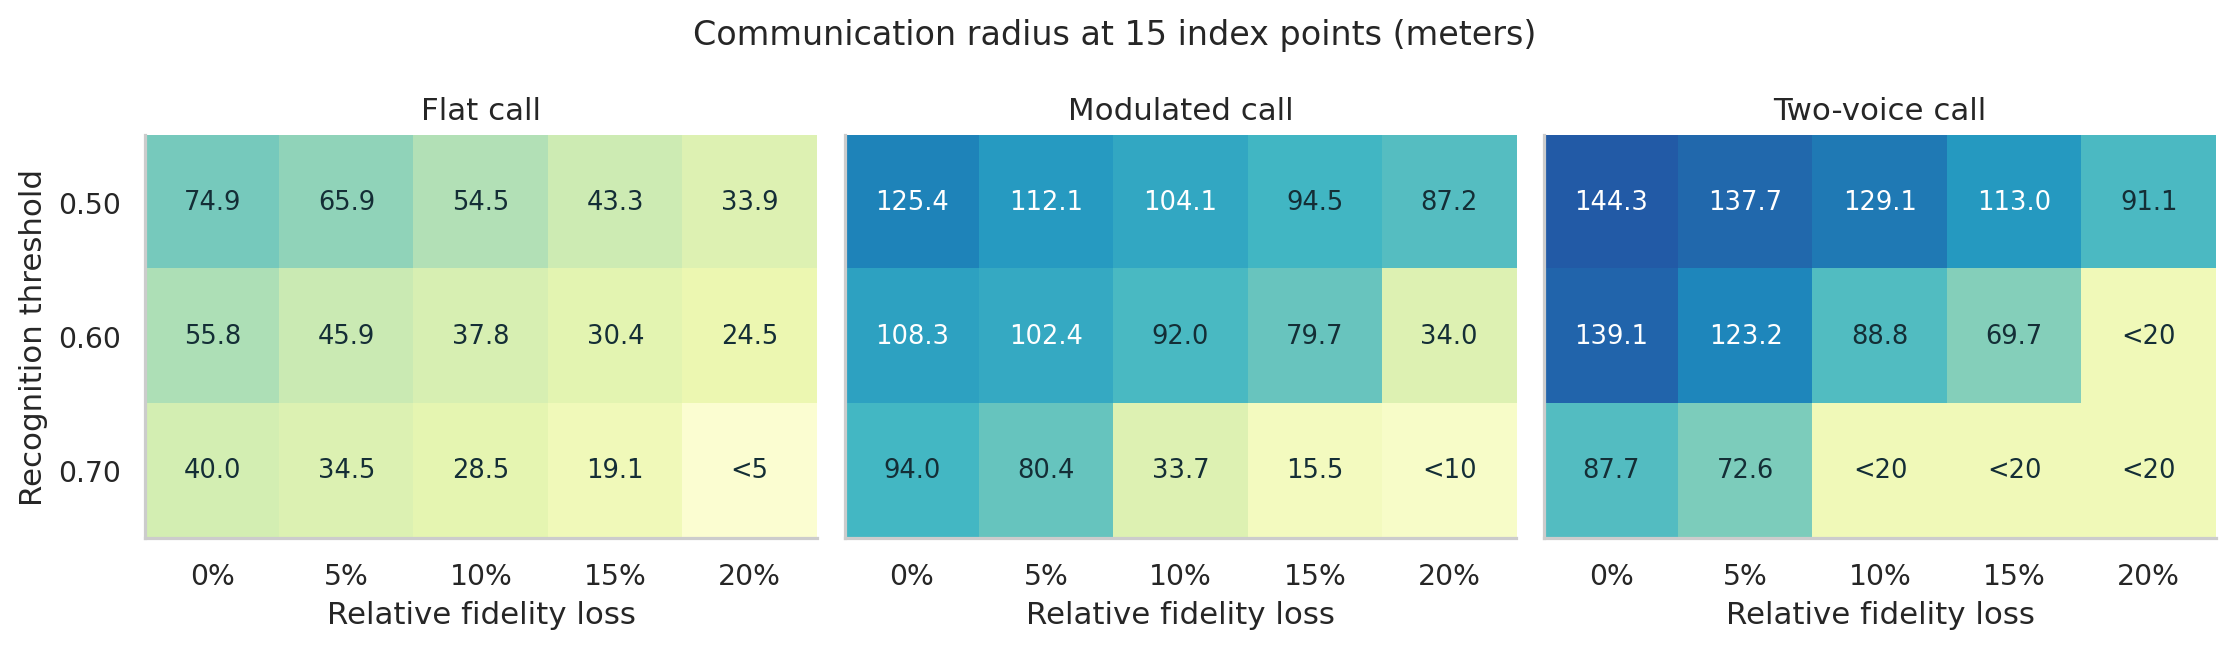
\includegraphics[width=\linewidth,height=.22\textheight,keepaspectratio]{../outputs_p4_part2/figures/02_effective_radius.png}\par\smallskip
    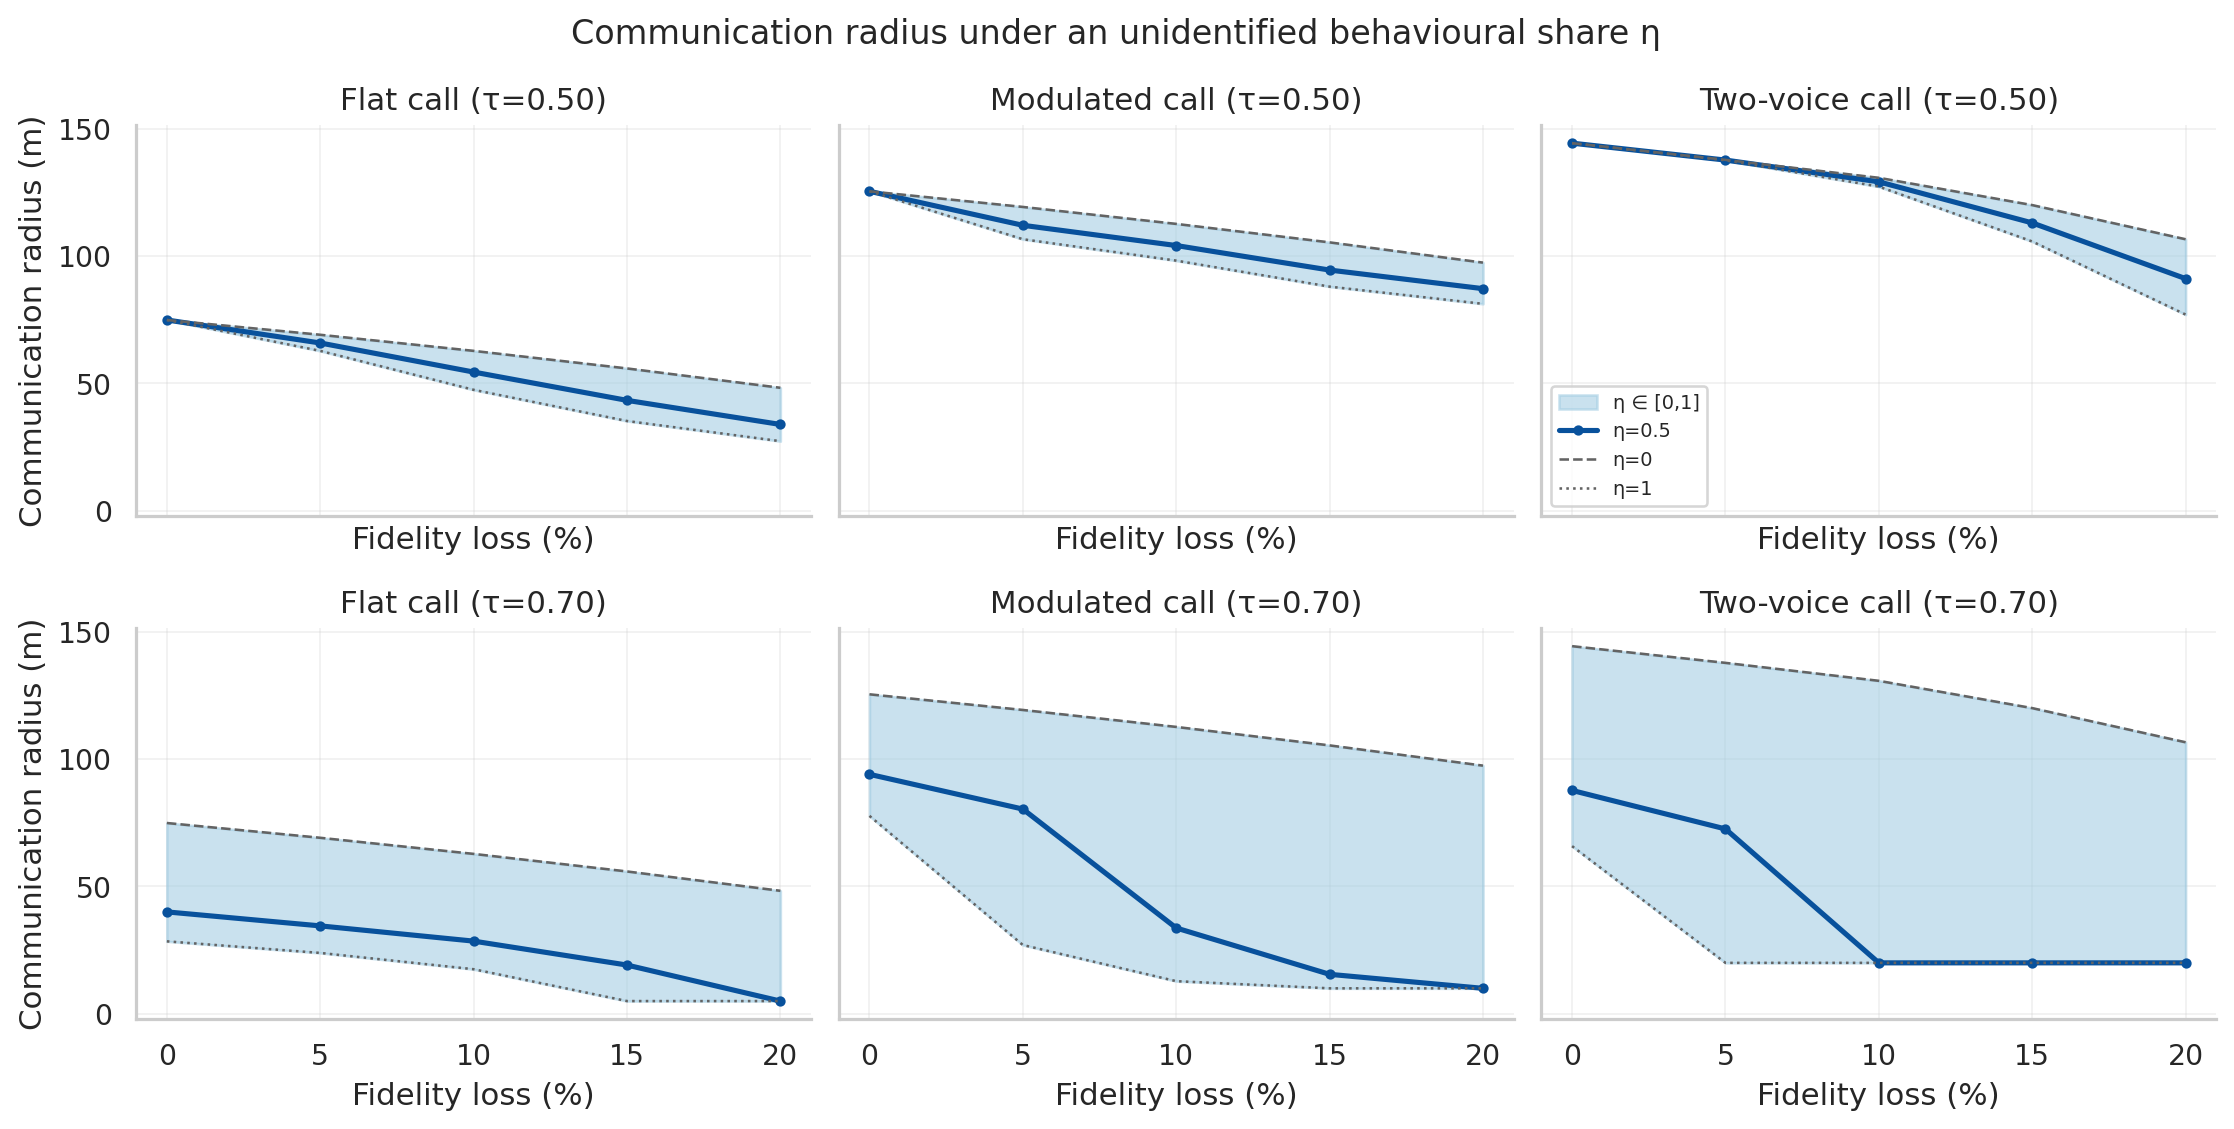
\includegraphics[width=\linewidth,height=.25\textheight,keepaspectratio]{../outputs_p4_part2/figures/05_eta_band.png}
    \caption{$15$ 个压力情景下的 $15$ 分综合通信半径热图（上）及未识别参数 $\eta \in [0,1]$ 下的通信半径带（下）}
    \label{fig:p4_stress}
\end{figure}

\subsection{阶段四：未来回放实验改进与栖息地声学保护建议}

针对本研究全流程暴露的样本与机制局限，提出以下\textbf{未来回放实验改进方案}：
\begin{enumerate}
    \item \textbf{个体级追踪以识别参与比例 $\rho$}：现有记录仅判断群体是否响应，导致无法验证 $\rho$；建议引入无人机航拍或多视角同步录像，逐只统计响应个体数与行为先后顺序，并结合生物声学标签区分``未感知''与``已感知但未外显响应''。
    \item \textbf{同步量化背景噪声与海况以标定 $\eta$}：现缺声压级（dB）、风速与浪高观测，致使 $\eta$ 及 $(\tau,\delta)$ 到物理噪声的映射不可识别；未来实验须在回放点同步布设水听器/麦克风记录实时环境噪声谱，实现噪声分贝到行为衰减的直接标定。
    \item \textbf{扩充独立音轨与加密中远距离采样}：增加不同个体录制的独立自然音轨以消除跨实验复用带来的伪重复，同时在 $64\text{--}256\text{ m}$ 区间增加重复试次，缓解双声型在中远距离高达 $30\%\text{--}36.7\%$ 的信息性缺失。
\end{enumerate}

从控制声学干扰出发，结合上述量化半径与面积损失规律，对非洲企鹅沿海觅食栖息地提出以下\textbf{保护管理建议及其适用条件与局限性}：
\begin{enumerate}
    \item \textbf{划定核心觅食区 $150\text{--}200\text{ m}$ 声学缓冲带}：依据 \texttt{mod}（$125.4\text{ m}$）与 \texttt{tv}（$144.3\text{ m}$，搜寻情境达 $171.9\text{ m}$）的有效通信半径，在已知沿海水域觅食热点周边划定至少 $150\text{--}200\text{ m}$ 的船只避让与低噪缓冲区，保障群体远距离声学联络与集结功能。
    \item \textbf{实施搜寻高峰期船只限速与声源降噪管控}：第三、四问均显示企鹅在搜寻情境下响应最活跃，且环境恶化对近源平直型叫声的边际破坏最剧烈（相关性降 $20\%$ 即损失 $80\%$ 通信面积）；建议在晨间出航与觅食搜寻高峰时段，对经过栖息地周边的商业与观光船只实施限速、静音推进及航道外移，重点削减与企鹅基频及三倍频（$250\text{--}1100\text{ Hz}$）重叠的低中频船只噪声。
    \item \textbf{适用条件与局限性}：上述建议适用于非洲企鹅海面觅食、通勤与搜寻阶段（不直接涵盖陆地繁殖期或水下潜泳通信）；受限于现有数据未建立相关性损失 $\delta$ 与船只噪声分贝（dB）的物理转换关系、且行为敏感份额 $\eta$ 存在不确定区间，缓冲带宽度与限速分贝标准在落地前须结合当地海域声场实测进行二次标定，并避免依赖单一叫声类型制定保护红线。
\end{enumerate}
\clearpage

\section{模型评价与改进}
\draftnote{报告按日期验证、改变保真度权重与识别阈值、改变响应个体占比后的结果。结合样本分布，讨论后续如何记录背景噪声、平衡各距离的回放次数，并统计群内作出反应的个体数。}
\subsection*{主要结论}
\draftnote{逐问给出定量结论及适用条件，再写一项有实验依据的保护建议。}
\setcounter{secnumdepth}{0}\renewcommand{\refname}{参考文献}
\begin{thebibliography}{9}
\bibitem{problem} 2026 年亚太地区大学生数学建模竞赛 C 题：《非洲企鹅在海上的声学通信与回放响应》（题名中译）。
\bibitem{data} C 题配套数据，Zenodo 记录 21376649。\url{https://zenodo.org/records/21376649}.
\end{thebibliography}
\appendix
\section*{附录：支撑材料}
\phantomsection\addcontentsline{toc}{section}{附录：支撑材料}
\draftnote{记录软件版本、随机种子、清洗规则、交叉验证分组、曲线拟合参数、删失假设和生成最终图表的命令。}
\end{document}


